% !TEX root
%
% Copyright (c) 2018-2019  OpenCyphal
%

\documentclass{cyphaldoc}

\usepackage{multirow}
\usepackage{tabularx}
\usepackage{amsmath}
\usepackage{amssymb}
\usepackage{amsfonts}
\usepackage{longtable}
\usepackage{diagbox}

\urlstyle{same}

% This macro embeds the selected DSDL definition or the contents of a DSDL namespace into the document.
% It accepts one mandatory argument which is either a full DSDL type name, e.g. uavcan.node.Heartbeat,
% or a full type name glob expression, e.g., uavcan.node.*.
\newcommand{\DSDL}[1]{%
    % Clean up beforehand to ensure clean initial state.
    \immediate\write18{rm -f ../*.tmp}%
    % Invoke the target command and save the useful output into a file; ignore error output
    \immediate\write18{../render_dsdl.py #1 > ../dsdl.tmp}%
    % Now, if the above command has failed, the output file would be empty. We remove empty file to escalate error.
    % Escalation is very important as it allows us to abort compilation on failure instead of generating invalid
    % documents silently.
    \immediate\write18{find .. -type f -name '*.tmp' -size 0 -delete}%
    % Read the file. This command fails if the file was empty, which is exactly want we want.
    \immediate\chapter{Data structure description language}\label{sec:dsdl}

The data structure description language, or \emph{DSDL}, is a simple domain-specific language designed for
defining composite data types.
The defined data types are used for exchanging data between Cyphal nodes via one of the standard Cyphal
transport protocols\footnote{The standard transport protocols are documented in chapter~\ref{sec:transport}.
Cyphal doesn't prohibit users from defining their own application-specific transports as well,
although users doing that are likely to encounter compatibility issues and possibly a suboptimal
performance of the protocol.}.

\section{Architecture}

\subsection{General principles}

In accordance with the UAVCAN architecture, DSDL allows users to define data types of two kinds:
message and service.
\emph{Message types} are used to exchange data over publish-subscribe one-to-many message links identified by subject-ID,
and \emph{service types} are used to perform request-response one-to-one exchanges (like RPC) identified by service-ID.
A message data type defines one data schema of the message object,
and a service data type contains two independent data schema definitions.
One of them applies to the request object (transferred from client to server),
and the other applies to the response object (transferred from the server back to the client).

Following the deterministic nature of UAVCAN, the size of a serialized representation of any
message or service object is bound within statically known limits.
Variable-size entities always have a fixed size limit defined by the data type designer.

DSDL definitions are strongly statically typed.

DSDL provides a well-defined means of data type versioning, which enables data type maintainers to introduce changes
to released data types while ensuring backward compatibility with fielded systems.

DSDL is designed to support extensive static analysis. Important properties of data type definitions such as
backward binary compatibility and data field layouts can be checked and validated by automatic software tools
before the systems utilizing them are fielded.

DSDL definitions can be used to automatically generate serialization (and deserialization) source code
for any data type in a target programming language.
A tool that is capable of generating serialization code based on a DSDL definition is called a \emph{DSDL compiler}.
More generically, a software tool designed for working with DSDL definitions is called a
\emph{DSDL processing tool}.

\subsection{Data types and namespaces}

Every data type is located inside a \emph{namespace}.
Namespaces may be included into higher-level namespaces, forming a tree hierarchy.

A namespace that is at the root of the tree hierarchy (i.e., not nested within another one)
is called a \emph{root namespace}.
A namespace that is located inside another namespace is called a \emph{nested namespace}.

A data type is uniquely identified by its namespaces and its \emph{short name}.
The short name of a data type is the name of the type itself excluding the containing namespaces.

A \emph{full name} of a data type consists of its short name and all of its namespace names.
The short name and the namespace names included in a full name are called \emph{name components}.
Name components are ordered: the root namespace is always the first component of the name,
followed by the nested namespaces, if there are any, in the order of their nesting;
the short name is always the last component of the full name.
The full name is formed by joining its name components via the ASCII dot character ``\verb|.|'' (ASCII code 46).

A \emph{full namespace} name is the full name without the short name and its component separator.

A \emph{sub-root namespace} is a nested namespace that is located immediately under its root namespace.
Data types that reside directly under their root namespace do not have a sub-root namespace.

The name structure is illustrated on the figure \ref{fig:dsdl_data_type_name_structure}.

\begin{figure}[H]
    $$
    \overbrace{
        \underbrace{
            \underbrace{\texttt{\huge{uavcan}}}_{\substack{\text{root} \\ \text{namespace}}}%
            \texttt{\huge{.}}%
            \underbrace{\texttt{\huge{node}}}_{\substack{\text{nested, also} \\ \text{sub-root} \\ \text{namespace}}}%
            \texttt{\huge{.}}%
            \underbrace{\texttt{\huge{port}}}_{\substack{\text{nested} \\ \text{namespace}}}%
        }_{\text{full namespace}}%
        \texttt{\huge{.}}%
        \underbrace{\texttt{\huge{GetInfo}}}_{\text{short name}}
    }^{\text{full name}}
    $$
    \caption{Data type name structure.\label{fig:dsdl_data_type_name_structure}}
\end{figure}

The following rules apply to naming: 

\begin{itemize}
    \item A set of full namespace names and a set of full data type names must not intersect\footnote{%
    For example, a namespace ``\texttt{vendor.example}'' and a data type ``\texttt{vendor.example.1.0}''
    are mutually exclusive.
    Note the data type name shown in this example violates the naming conventions
    which are reviewed in a separate section.
}.
    \item Data type names and namespace names are case-sensitive. Names that differ only in letter case are not permitted because that may cause name collisions within case-insensitive file systems.
    \item A name component consists of alphanumeric ASCII characters (\verb|A-Z|, \verb|a-z|, and \verb|0-9|) and underscores (``\verb|_|'', ASCII code 95).
    \item The first character of a name must not be numerical.
    \item An empty string is not a valid name.
    \item File name extension ``\verb|uavcan|'' (mandatory).
    \item A name component must not match any of the reserved word patterns listed in table \ref{table:dsdl_reserved_word_patterns}.
    \item The length of a full data type name must not exceed 50 characters, including the name component separators.
\end{itemize}

Every data type definition is assigned a major and minor version number pair.
In order to uniquely identify a data type definition, its version numbers must be specified.
In the following text, the term \emph{version} without a majority qualifier refers to
a pair of major and minor version numbers.

Valid data type version numbers range from 0 to 255, inclusively.
A data type version where both major and minor components are zero is not allowed.

\subsection{File hierarchy}

DSDL data type definitions are contained in UTF-8 encoded text files with \verb|.uavcan| file extensions.

One file defines exactly one version of a data type,
meaning that each combination of major and minor version numbers must be unique per data type name.
There may be any number of versions of the same data type defined alongside each other,
provided that each version is defined once at most.
Version numbers can be non-contiguous,
meaning that it is allowed to skip version numbers or remove existing definitions as long as they are neither the oldest nor newest versions.

A data type definition may have an optional fixed port-ID\footnote{Chapter \ref{sec:basic_concepts}.} value specified.

The name of a data type definition file is constructed from the following entities
joined via the ASCII dot character ``\verb|.|'' (ASCII code 46), in the specified order:
\begin{itemize}
    \item Fixed port-ID in decimal notation (optional).
    \item Short name of the data type (mandatory, always non-empty).
    \item Major version number in decimal notation (mandatory).
    \item Minor version number in decimal notation (mandatory).
    \item File name extension ``\verb|uavcan|'' (mandatory).
\end{itemize}

\begin{figure}[H]
    $$
    \overbrace{%
        \underbrace{\texttt{\huge{432}}}_{\substack{\text{fixed} \\ \text{port-ID}}}%
        \texttt{\huge{.}}%
    }^{\text{optional}}%
    \overbrace{%
        \underbrace{\texttt{\huge{GetInfo}}}_{\substack{\text{short name}}}%
        \texttt{\huge{.}}%
        \underbrace{\texttt{\huge{1.0}}}_{\substack{\text{version} \\ \text{numbers}}}%
        \texttt{\huge{.}}%
        \underbrace{\texttt{\huge{uavcan}}}_{\text{file extension}}%
    }^{\text{mandatory}}
    $$
    \caption{Data type definition file name structure.\label{fig:dsdl_definition_file_name_structure}}
\end{figure}

DSDL namespaces are represented as directories, where one directory defines exactly one namespace, possibly nested.
The name of the directory defines the name of its data type name component.
A directory defining a namespace will always define said namespace in its entirety,
meaning that the contents of a namespace cannot be spread across different directories sharing the same name.
One directory cannot define more than one level of
nesting\footnote{For example, ``\texttt{foo.bar}'' is not a valid directory name.
The valid representation would be ``\texttt{bar}'' nested in ``\texttt{foo}''.}.

\begin{remark}
    \begin{figure}[H]
        \begin{tabu}{|l|X|} \hline
            \rowfont{\bfseries}
            Directory tree & Entry description \\\hline

            \texttt{vendor\_x/} &
            Root namespace \texttt{vendor\_x}. \\\cline{2-2}

            \texttt{\qquad{}foo/} &
            Nested namespace (also sub-root) \texttt{vendor\_x.foo}. \\\cline{2-2}

            \texttt{\qquad{}\qquad{}100.Run.1.0.uavcan} &
            Data type definition v1.0 with fixed service-ID 100. \\\cline{2-2}

            \texttt{\qquad{}\qquad{}100.Status.1.0.uavcan} &
            Data type definition v1.0 with fixed subject-ID 100. \\\cline{2-2}

            \texttt{\qquad{}\qquad{}ID.1.0.uavcan} &
            Data type definition v1.0 without fixed port-ID. \\\cline{2-2}

            \texttt{\qquad{}\qquad{}ID.1.1.uavcan} &
            Data type definition v1.1 without fixed port-ID. \\\cline{2-2}

            \texttt{\qquad{}\qquad{}bar\_42/} &
            Nested namespace \texttt{vendor\_x.foo.bar\_42}. \\\cline{2-2}

            \texttt{\qquad{}\qquad{}\qquad{}101.List.1.0.uavcan} &
            Data type definition v1.0 with fixed service-ID 101. \\\cline{2-2}

            \texttt{\qquad{}\qquad{}\qquad{}102.List.2.0.uavcan} &
            Data type definition v2.0 with fixed service-ID 102. \\\cline{2-2}

            \texttt{\qquad{}\qquad{}\qquad{}ID.1.0.uavcan} &
            Data type definition v1.0 without fixed port-ID. \\\hline
        \end{tabu}
        \caption{DSDL directory structure example.}\label{fig:dsdl_directory_structure_example}
    \end{figure}
\end{remark}

\subsection{Elements of data type definition}

A data type definition file contains an exhaustive description of a particular version of the data type in the
\emph{data structure description language} (DSDL).
As explained above, one data type definition contains one schema definition for message types or two schema definitions for service types.

A data schema definition contains an ordered, possibly empty collection of \emph{field attributes} and/or
unordered, possibly empty collection of \emph{constant attributes}.
A data schema may describe either a \emph{structure object} or a \emph{tagged union object}.
The value of a structure object is a function of the values of all of its field attributes.
A tagged union object is formed from at least two field attributes,
but it is capable of holding exactly one field attribute value at any given time.
The value of a tagged union object is a function of the field attribute values
it is presently holding and the value of these field attributes.

A field attribute represents a named dynamically assigned value of a statically defined type
that can be exchanged over the network as a member of its containing object.
A padding field attribute is a special kind of field attribute which is used for data alignment purposes;
such field attributes are not named.

A constant attribute represents a named statically defined value of a statically defined type.
Constants are never exchanged over the network, since they are assumed to all involve nodes
by virtue of them sharing compatible definitions of the data type.

Constant values are defined via \emph{DSDL expressions},
which are evaluated at the time of DSDL definition processing.
There is a special category of types called \emph{expression types},
instances of which are used only during expression evaluation
and cannot be exchanged over the network.

Data type definitions can also contain various auxiliary elements reviewed later,
such as deprecation markers (notifying its users that the data type is no longer recommended for new designs)
or assertions (special statements introduced by data type designers
which are statically validated by DSDL processing tools).

\subsection{Serialization}

Every object that can be exchanged between UAVCAN nodes has a well-defined \emph{serialized representation}.
The value and meaning of an object can be unambiguously recovered from its serialized representation,
provided that the object type is known.

\label{sec:dsdl_bit_length_set}
A serialized representation is a sequence of binary digits (bits);
the number of bits in a serialized representation is called its \emph{bit length}.
A \emph{bit length set} of a data type (or a data schema) refers to the set of bit length values of all possible
serialized representations of objects that are instances of the data type (or that follow the data schema).

The data type of a serialized message or service object exchanged over the network
is recovered from its subject-ID or service-ID, respectively,
which is attached to the serialized object, along with other metadata, in a manner dictated by the applicable
transport layer specification (chapter \ref{sec:transport_layer}).
For more information on port identifiers and data type mapping refer to section \ref{sec:basic_subjects_and_services}.

\section{Grammar}\label{sec:dsdl_grammar}

This section contains the formal definition of the DSDL grammar.
Its notation is introduced beforehand.
The meaning of each element of the grammar and their semantics will be explained in the following sections.

\subsection{Notation}

The following definition relies on the PEG\footnote{Parsing expression grammar.}
notation described in table~\ref{table:dsdl_grammar_definition_notation}%
\footnote{%
    Inspired by Parsimonious -- an MIT-licensed software product authored by Erik Rose;
    its sources are available at \url{https://github.com/erikrose/parsimonious}.
}.
The text of the formal definition contains comments which begin with an octothorp and last until the end of the line.

\begin{CyphalSimpleTable}{Notation used in the formal grammar definition}{|l X|}
    \label{table:dsdl_grammar_definition_notation}
    Pattern & Description \\

    \texttt{"text"} &
    Denotes a terminal string of ASCII characters.
    The string is case-sensitive. \\

    \emph{(space)} &
    Concatenation.
    E.g., \texttt{korovan paukan excavator} matches a sequence where the specified tokens
    appear in the defined order. \\

    \texttt{abc / ijk / xyz} &
    Alternatives.
    The leftmost matching alternative is accepted. \\

    \texttt{abc?} &
    Optional greedy match. \\

    \texttt{abc*} &
    Zero or more expressions, greedy match. \\

    \texttt{abc+} &
    One or more expressions, greedy match. \\

    \texttt{\textasciitilde{}r"regex"} &
    An IEEE POSIX Extended Regular Expression pattern defined between the double quotes.
    The expression operates on the ASCII character set and is always case-sensitive.
    ASCII escape sequences ``\texttt{\textbackslash{}r}'', ``\texttt{\textbackslash{}n}'', and
    ``\texttt{\textbackslash{}t}'' are used to denote ASCII carriage return (code 13),
    line feed (code 10), and tabulation (code 9) characters, respectively. \\

    \texttt{\textasciitilde{}r'regex'} &
    As above, with single quotes instead of double quotes. \\

    \texttt{(abc xyz)} &
    Parentheses are used for grouping. \\
\end{CyphalSimpleTable}

\subsection{Definition}

At the top level, a DSDL definition file is an ordered collection of statements;
the order is determined by the relative placement of statements inside the DSDL source file:
statements located closer the beginning of the file precede those that are located closer to the end of the file.

From the top level down to the expression rule, the grammar is a valid regular grammar,
meaning that it can be parsed using standard regular expressions.

The grammar definition provided here assumes lexerless parsing;
that is, it applies directly to the unprocessed source text of the definition.

All characters used in the definition belong to the ASCII character set.

\clearpage\inputminted[fontsize=\scriptsize]{python}{dsdl/grammar.parsimonious}

\subsection{Expressions}

Symbols representing operators belong to the ASCII (basic Latin) character set.

Operators of the same precedence level are evaluated from left to right.

The attribute reference operator is a special case: it is defined for an instance of any type
on its left side and an attribute identifier on its right side.
The concept of ``attribute identifier'' is not otherwise manifested in the type system.
The attribute reference operator is not explicitly documented for any data type;
instead, the documentation specifies the set of available attributes for instances of said type,
if there are any.

\begin{CyphalSimpleTable}{Unary operators}{|l l X|}
    Symbol                             & Precedence & Description \\
    \texttt{\textbf{+}}                         & 3 & Unary plus \\
    \texttt{\textbf{-}} (hyphen-minus)          & 3 & Unary minus \\
    \texttt{\textbf{!}}                         & 8 & Logical not \\
\end{CyphalSimpleTable}

\begin{CyphalSimpleTable}{Binary operators}{|l l X|}
    Symbol                                          & Precedence & Description \\
    \texttt{\textbf{.}} (full stop)                          & 1 & Attribute reference
                                                                   (parent object on the left side,
                                                                   attribute identifier on the right side) \\

    \texttt{\textbf{**}}                                     & 2 & Exponentiation
                                                                   (base on the left side, power on the right side) \\

    \texttt{\textbf{*}}                                      & 4 & Multiplication \\
    \texttt{\textbf{/}}                                      & 4 & Division \\
    \texttt{\textbf{\%}}                                     & 4 & Modulo \\

    \texttt{\textbf{+}}                                      & 5 & Addition \\
    \texttt{\textbf{-}} (hyphen-minus)                       & 5 & Subtraction \\

    \texttt{\textbf{|}} (vertical line)                      & 6 & Bitwise or \\
    \texttt{\textbf{\textasciicircum{}}} (circumflex accent) & 6 & Bitwise xor \\
    \texttt{\textbf{\&}}                                     & 6 & Bitwise and \\

    \texttt{\textbf{==}} (dual equals sign)                  & 7 & Equality \\
    \texttt{\textbf{!=}}                                     & 7 & Inequality \\
    \texttt{\textbf{<=}}                                     & 7 & Less or equal \\
    \texttt{\textbf{>=}}                                     & 7 & Greater or equal \\
    \texttt{\textbf{<}}                                      & 7 & Less \\
    \texttt{\textbf{>}}                                      & 7 & Greater \\

    \texttt{\textbf{||}} (dual vertical line)                & 9 & Logical or \\
    \texttt{\textbf{\&\&}}                                   & 9 & Logical and \\
\end{CyphalSimpleTable}

\subsection{Literals}

Upon its evaluation, a literal yields an object of a particular type depending on the syntax of the literal,
as specified in this section.

\subsubsection{Boolean literals}

A boolean literal is denoted by the keyword ``\verb|true|'' or ``\verb|false|''
represented by an instance of primitive type ``\verb|bool|'' (section~\ref{sec:dsdl_primitive_types})
with an appropriate value.

\subsubsection{Numeric literals}

Integer and real literals are represented as instances of type ``\verb|rational|'' (section~\ref{sec:dsdl_rational}).

The digit separator character ``\verb|_|'' (underscore) does not affect the interpretation of numeric literals.

The significand of a real literal is formed by the integer part, the optional decimal point,
and the optional fraction part;
either the integer part or the fraction part (not both) can be omitted.
The exponent is optionally specified after the letter ``\verb|e|'' or ``\verb|E|'';
it indicates the power of 10 by which the significand is to be scaled.
Either the decimal point or the letter ``\verb|e|''/``\verb|E|'' with the following exponent
(not both) can be omitted from a real literal.

\begin{remark}
    An integer literal \verb|0x123| is represented internally as $\frac{291}{1}$.

    A real literal \verb|.3141592653589793e+1| is represented internally as
    $\frac{3141592653589793}{1000000000000000}$.
\end{remark}

\subsubsection{String literals}

String literals are represented as instances of type ``\verb|string|'' (section~\ref{sec:dsdl_string}).

A string literal is allowed to contain an arbitrary sequence of Unicode characters,
excepting escape sequences defined in table~\ref{table:dsdl_string_literal_escape}
which shall follow one of the specified therein forms.
An escape sequence begins with the ASCII backslash character ``\verb|\|''.

\begin{CyphalSimpleTable}{String literal escape sequences}{|l X|}
    Sequence & Interpretation
    \label{table:dsdl_string_literal_escape} \\

    \texttt{\textbackslash{}\textbackslash{}}   & Backslash, ASCII code 92. Same as the escape character. \\
    \texttt{\textbackslash{}r}                  & Carriage return, ASCII code 13.               \\
    \texttt{\textbackslash{}n}                  & Line feed, ASCII code 10.                     \\
    \texttt{\textbackslash{}t}                  & Horizontal tabulation, ASCII code 9.          \\

    \texttt{\textbackslash{}\textquotesingle{}} &
    Apostrophe (single quote), ASCII code 39. Regardless of the type of quotes around the literal. \\

    \texttt{\textbackslash{}\textquotedbl{}}    &
    Quotation mark (double quote), ASCII code 34. Regardless of the type of quotes around the literal. \\

    \texttt{\textbackslash{}u????} &
    Unicode symbol with the code point specified by a four-digit hexadecimal number.
    The placeholder ``\texttt{?}'' represents a hexadecimal character \texttt{[0-9a-fA-F]}. \\

    \texttt{\textbackslash{}U????????} &
    Like above, the code point is specified by an eight-digit hexadecimal number. \\

\end{CyphalSimpleTable}

\begin{remark}
    \begin{minted}{python}
        @assert "oh,\u0020hi\U0000000aMark" == 'oh, hi\nMark'
    \end{minted}
\end{remark}

\subsubsection{Set literals}

Set literals are represented as instances of type ``\verb|set|'' (section~\ref{sec:dsdl_set})
parameterized by the type of the contained elements which is determined automatically.

A set literal declaration shall specify at least one element,
which is used to determine the element type of the set.

The elements of a set literal are defined as DSDL expressions which are evaluated before a set is constructed
from the corresponding literal.

\begin{remark}
    \begin{minted}{python}
        @assert {"cells", 'interlinked'} == {"inter" + "linked", 'cells'}
    \end{minted}
\end{remark}

\subsection{Reserved identifiers}\label{sec:dsdl_reserved_identifiers}

DSDL identifiers and data type name components that match any of the
case-insensitive patterns specified in table~\ref{table:dsdl_reserved_word_patterns}
cannot be used to name new entities.
The semantics of such identifiers is predefined by the DSDL specification,
and as such, they cannot be used for other purposes.
Some of the reserved identifiers do not have any functions associated with them
in this version of the DSDL specification, but this may change in the future.

\begin{CyphalSimpleTable}{Reserved identifier patterns (POSIX ERE notation, ASCII character set, case-insensitive)}%
    {|l l X|}%
    \label{table:dsdl_reserved_word_patterns}%
    POSIX ERE ASCII pattern                            & Example            & Special meaning \\
    \texttt{truncated}                                 &                    & Cast mode specifier \\
    \texttt{saturated}                                 &                    & Cast mode specifier \\
    \texttt{true}                                      &                    & Boolean literal \\
    \texttt{false}                                     &                    & Boolean literal \\
    \texttt{bool}                                      &                    & Primitive type category \\
    \texttt{u?int\textbackslash{}d*}                   & \texttt{uint8}     & Primitive type category \\
    \texttt{float\textbackslash{}d*}                   & \texttt{float}     & Primitive type category \\
    \texttt{u?q\textbackslash{}d+\_\textbackslash{}d+} & \texttt{q16\_8}    & Primitive type category (future) \\
    \texttt{void\textbackslash{}d*}                    & \texttt{void}      & Void type category \\
    \texttt{optional}                                  &                    & Reserved for future use \\
    \texttt{aligned}                                   &                    & Reserved for future use \\
    \texttt{const}                                     &                    & Reserved for future use \\
    \texttt{struct}                                    &                    & Reserved for future use \\
    \texttt{super}                                     &                    & Reserved for future use \\
    \texttt{template}                                  &                    & Reserved for future use \\
    \texttt{enum}                                      &                    & Reserved for future use \\
    \texttt{self}                                      &                    & Reserved for future use \\
    \texttt{and}                                       &                    & Reserved for future use \\
    \texttt{or}                                        &                    & Reserved for future use \\
    \texttt{not}                                       &                    & Reserved for future use \\
    \texttt{auto}                                      &                    & Reserved for future use \\
    \texttt{type}                                      &                    & Reserved for future use \\
    \texttt{con}                                       &                    & Compatibility with Microsoft Windows \\
    \texttt{prn}                                       &                    & Compatibility with Microsoft Windows \\
    \texttt{aux}                                       &                    & Compatibility with Microsoft Windows \\
    \texttt{nul}                                       &                    & Compatibility with Microsoft Windows \\
    \texttt{com\textbackslash{}d}                      & \texttt{com1}      & Compatibility with Microsoft Windows \\
    \texttt{lpt\textbackslash{}d}                      & \texttt{lpt9}      & Compatibility with Microsoft Windows \\
    \texttt{\_.*\_}                                    & \texttt{\_offset\_}& Special-purpose intrinsic entities \\
\end{CyphalSimpleTable}

\subsection{Reserved comment forms}\label{sec:dsdl_reserved_comment}

Line comments that match the following regular expression are reserved for vendor-specific language extensions:
\verb|^#\[.+\].*|

\begin{remark}
    \begin{minted}{python}
        #[canadensis(enum_start)] all of this line is part of the reserved form.
        # After the newline this comment is now a regular DSDL comment.
    \end{minted}
\end{remark}

\section{Expression types}\label{sec:dsdl_expression_types}

Expression types are a special category of data types whose instances can only exist and be operated upon
at the time of DSDL definition processing.
As such, expression types cannot be used to define attributes,
and their instances cannot be exchanged between nodes.

Expression types are used to represent values of constant expressions which are evaluated
when a DSDL definition is processed.
Results of such expressions can be used to define various constant properties,
such as array length boundaries or values of constant attributes.

Expression types are specified in this section.
Each expression type has a formal DSDL name for completeness;
even if such types can't be used to define attributes,
a well-defined formal name allows DSDL processing tools to emit well-formed
and understandable diagnostic messages.

\subsection{Rational number}\label{sec:dsdl_rational}

At the time of DSDL definition processing, integer and real numbers are represented internally as rational numbers
where the range of numerator and denominator is unlimited\footnote{%
    Technically, the range may only be limited by the memory resources available to the DSDL processing tool.
}.
DSDL processing tools are not permitted to introduce any implicit rational number transformations that
may result in a loss of information.

The DSDL name of the rational number type is ``\verb|rational|''.

Rational numbers are assumed to be stored in a normalized form, where the denominator is positive
and the greatest common divisor of the numerator and the denominator is one.

A rational number can be used in a context where an integer value is expected only if its denominator equals one.

Implicit conversions between boolean-valued entities and rational numbers are not allowed.

\begin{CyphalSimpleTable}{Operators defined on instances of rational numbers}{|l l X X|}
    Op & Type & Constraints & Description
    \label{table:dsdl_operators_rational} \\

    \texttt{\textbf{+}}     & $(\texttt{rational}) \rightarrow \texttt{rational}$ & &
    No effect. \\
    \texttt{\textbf{-}}     & $(\texttt{rational}) \rightarrow \texttt{rational}$ & &
    Negation. \\

    \texttt{\textbf{**}}    & $(\texttt{rational}, \texttt{rational}) \rightarrow \texttt{rational}$ &
    Power denominator equals one &
    Exact exponentiation. \\

    \texttt{\textbf{**}}    & $(\texttt{rational}, \texttt{rational}) \rightarrow \texttt{rational}$ &
    Power denominator greater than one &
    Exponentiation with imp\-lem\-en\-ta\-ti\-on-de\-fin\-ed accuracy. \\

    \texttt{\textbf{*}}  & $(\texttt{rational}, \texttt{rational}) \rightarrow \texttt{rational}$ & &
    Exact multiplication. \\

    \texttt{\textbf{/}}  & $(\texttt{rational}, \texttt{rational}) \rightarrow \texttt{rational}$ &
    Non-zero divisor &
    Exact division. \\

    \texttt{\textbf{\%}} & $(\texttt{rational}, \texttt{rational}) \rightarrow \texttt{rational}$ &
    Non-zero divisor &
    Exact modulo. \\

    \texttt{\textbf{+}}  & $(\texttt{rational}, \texttt{rational}) \rightarrow \texttt{rational}$ & &
    Exact addition. \\

    \texttt{\textbf{-}}  & $(\texttt{rational}, \texttt{rational}) \rightarrow \texttt{rational}$ & &
    Exact subtraction. \\

    \texttt{\textbf{|}}  & $(\texttt{rational}, \texttt{rational}) \rightarrow \texttt{rational}$ &
    Denominators equal one &
    Bitwise or. \\

    \texttt{\textbf{\textasciicircum{}}} & $(\texttt{rational}, \texttt{rational}) \rightarrow \texttt{rational}$ &
    Denominators equal one &
    Bitwise xor. \\

    \texttt{\textbf{\&}} & $(\texttt{rational}, \texttt{rational}) \rightarrow \texttt{rational}$ &
    Denominators equal one &
    Bitwise and. \\

    \texttt{\textbf{!=}} & $(\texttt{rational}, \texttt{rational}) \rightarrow \texttt{bool}$ & & Exact inequality. \\
    \texttt{\textbf{==}} & $(\texttt{rational}, \texttt{rational}) \rightarrow \texttt{bool}$ & & Exact equality. \\
    \texttt{\textbf{<=}} & $(\texttt{rational}, \texttt{rational}) \rightarrow \texttt{bool}$ & & Less or equal. \\
    \texttt{\textbf{>=}} & $(\texttt{rational}, \texttt{rational}) \rightarrow \texttt{bool}$ & & Greater or equal. \\
    \texttt{\textbf{<}}  & $(\texttt{rational}, \texttt{rational}) \rightarrow \texttt{bool}$ & & Strictly less. \\
    \texttt{\textbf{>}}  & $(\texttt{rational}, \texttt{rational}) \rightarrow \texttt{bool}$ & & Strictly greater. \\

\end{CyphalSimpleTable}

\subsection{Unicode string}\label{sec:dsdl_string}

This type contains a sequence of Unicode characters.
It is used to represent string literals internally.

The DSDL name of the Unicode string type is ``\verb|string|''.

A Unicode string containing one symbol whose code point is within $[0, 127]$
(i.e., an ASCII character) is implicitly convertible into a \verb|uint8|-typed constant attribute value,
where the value of the constant is to be equal the code point of the symbol.

\begin{CyphalSimpleTable}{Operators defined on instances of Unicode strings}{|l l X|}
    Op & Type & Description
    \label{table:dsdl_operators_string} \\

    \texttt{\textbf{+}}  & $(\texttt{string}, \texttt{string}) \rightarrow \texttt{string}$ &
    Concatenation. \\

    \texttt{\textbf{!=}} & $(\texttt{string}, \texttt{string}) \rightarrow \texttt{bool}$ &
    Inequality of Unicode NFC normalized forms.
    NFC stands for \emph{Normalization Form Canonical Composition} --
    one of standard Unicode normalization forms where characters are recomposed by canonical equivalence. \\

    \texttt{\textbf{==}} & $(\texttt{string}, \texttt{string}) \rightarrow \texttt{bool}$ &
    Equality of Unicode NFC normalized forms. \\

\end{CyphalSimpleTable}

The set of operations and conversions defined for Unicode strings is to be extended in future versions of
the specification.

\subsection{Set}\label{sec:dsdl_set}

A set type represents an unordered collection of unique objects.
All objects shall be of the same type.
Uniqueness of elements is determined by application of the equality operator ``\verb|==|''.

The DSDL name of the set type is ``\verb|set|''.

A set can be constructed from a set literal, in which case such set shall contain at least one element.

The attributes and operators defined on set instances are listed in the tables~\ref{table:dsdl_set_attributes}
and~\ref{table:dsdl_set_operators}, where $E$ represents the set element type.

\begin{CyphalSimpleTable}{Attributes defined on instances of sets}{|l l X X|}
    Name & Type & Constraints & Description
    \label{table:dsdl_set_attributes} \\

    \texttt{min} & $E$ &
    Operator ``\texttt{<}'' is defined \mbox{$(E, E) \rightarrow \texttt{bool}$} &
    Smallest element in the set determined by sequential application of the operator ``\texttt{<}''. \\

    \texttt{max} & $E$ &
    Operator ``\texttt{<}'' is defined \mbox{$(E, E) \rightarrow \texttt{bool}$} &
    Greatest element in the set determined by sequential application of the operator ``\texttt{<}''. \\

    \texttt{count} & \texttt{rational} & &
    Cardinality. \\

\end{CyphalSimpleTable}

\newcommand\SetElementwiseOperator[1]{%
    \texttt{\textbf{#1}} & $(\texttt{set}_\texttt{<E>}, E) \rightarrow \texttt{set}_\texttt{<R>}$ & $E$ is not a set &
    Elementwise $(E, E) \rightarrow R$.\\

    \texttt{\textbf{#1}} & $(E, \texttt{set}_\texttt{<E>}) \rightarrow \texttt{set}_\texttt{<R>}$ & $E$ is not a set &
    Elementwise $(E, E) \rightarrow R$.\\
}

\begin{CyphalSimpleTable}{Operators defined on instances of sets}{|l l l X|}%
    \label{table:dsdl_set_operators}%
    Op & Type & Constraints & Description \\

    \texttt{\textbf{==}} & $(\texttt{set}_\texttt{<E>}, \texttt{set}_\texttt{<E>}) \rightarrow \texttt{bool}$ & &
    Left equals right. \\

    \texttt{\textbf{!=}} & $(\texttt{set}_\texttt{<E>}, \texttt{set}_\texttt{<E>}) \rightarrow \texttt{bool}$ & &
    Left does not equal right. \\

    \texttt{\textbf{<=}} & $(\texttt{set}_\texttt{<E>}, \texttt{set}_\texttt{<E>}) \rightarrow \texttt{bool}$ & &
    Left is a subset of right. \\

    \texttt{\textbf{>=}} & $(\texttt{set}_\texttt{<E>}, \texttt{set}_\texttt{<E>}) \rightarrow \texttt{bool}$ & &
    Left is a superset of right. \\

    \texttt{\textbf{<}}  & $(\texttt{set}_\texttt{<E>}, \texttt{set}_\texttt{<E>}) \rightarrow \texttt{bool}$ & &
    Left is a proper subset of right. \\

    \texttt{\textbf{>}}  & $(\texttt{set}_\texttt{<E>}, \texttt{set}_\texttt{<E>}) \rightarrow \texttt{bool}$ & &
    Left is a proper superset of right. \\

    \texttt{\textbf{|}} &
    $(\texttt{set}_\texttt{<E>}, \texttt{set}_\texttt{<E>}) \rightarrow \texttt{set}_\texttt{<E>}$ & &
    Union. \\

    \texttt{\textbf{\textasciicircum{}}} &
    $(\texttt{set}_\texttt{<E>}, \texttt{set}_\texttt{<E>}) \rightarrow \texttt{set}_\texttt{<E>}$ & &
    Disjunctive union. \\

    \texttt{\textbf{\&}} &
    $(\texttt{set}_\texttt{<E>}, \texttt{set}_\texttt{<E>}) \rightarrow \texttt{set}_\texttt{<E>}$ & &
    Intersection. \\

    \SetElementwiseOperator{**}
    \SetElementwiseOperator{*}
    \SetElementwiseOperator{/}
    \SetElementwiseOperator{\%}
    \SetElementwiseOperator{+}
    \SetElementwiseOperator{-}

\end{CyphalSimpleTable}

\subsection{Serializable metatype}\label{sec:dsdl_metaserializable}

Serializable types (which are reviewed in section~\ref{sec:dsdl_serializable_types})
are instances of the serializable metatype.
This metatype is convenient for expression of various relations and attributes defined on serializable types.

The DSDL name of the serializable metatype is ``\verb|metaserializable|''.

Available attributes are defined on a per-instance basis.

\section{Serializable types}\label{sec:dsdl_serializable_types}

\subsection{General principles}

Values of the serializable type category can be exchanged between nodes over the UAVCAN network.
This is opposed to the expression types (section~\ref{sec:dsdl_expression_types}),
instances of which can only exist while DSDL definitions are being evaluated.
The data serialization rules are defined in section~\ref{sec:dsdl_data_serialization}.

\subsubsection{Alignment and padding}\label{sec:dsdl_serializable_alignment_padding}

For any serializable type,
its \emph{alignment} $A$ is defined as some positive integer number of bits such that the offset of a
serialized representation of an instance of this type relative to the origin of the
containing serialized representation (if any) is an integer multiple of $A$.

Given an instance of type whose alignment is $A$,
it is guaranteed that its serialized representation is always an integer multiple of $A$ bits long.

When constructing a serialized representation,
the alignment and length requirements are satisfied by means of \emph{padding},
which refers to the extension of a bit sequence with zero bits until
the resulting alignment or length requirements are satisfied.
During deserialization, the padding bits are ignored (skipped) irrespective of their value
(also see related section \ref{sec:dsdl_serialization_implicit_truncation}).

\begin{remark}
    For example, given a variable-length entity whose length varies between 1 and 3 bits,
    followed by a field whose type has the alignment requirement of 8,
    one may end up with 5, 6, or 7 bits of padding inserted before the second field at runtime.

    The exact amount of such padding cannot always be determined statically because it depends on the size of the
    preceding entity;
    however, it is guaranteed that it is always strictly less than the alignment requirement of the following field
    or, if this is the last field in a group, the alignment requirement of its container.
\end{remark}

\subsection{Void types}

Void types are used for padding purposes.
The alignment of void types is 1 bit (i.e., no alignment).

Void-typed field attributes are set to zero when an object is serialized and ignored when it is deserialized.
Void types can be used to reserve space in data type definitions for possible use in later versions of the data type.

The DSDL name pattern for void types is as follows: ``\verb|void[1-9]\d*|'',
where the trailing integer represents its width, in bits,
ranging from 1 to 64, inclusive.

Void types can be referred to directly by their name from any namespace.

\subsection{Primitive types}\label{sec:dsdl_primitive_types}

Primitive types are assumed to be known to DSDL processing tools a priori,
and as such, they need not be defined by the user.
Primitive types can be referred to directly by their name from any namespace.

The alignment of primitive types is 1 bit (i.e., no alignment).

\subsubsection{Hierarchy}

The hierarchy of primitive types is documented below.

\begin{itemize}
    \item \textbf{Boolean types.} A boolean-typed value represents a variable of the Boolean algebra.
    A Boolean-typed value can have two values: true and false.
    The corresponding DSDL data type name is ``\verb|bool|''.

    \item \textbf{Algebraic types.} Those are types for which conventional algebraic operators are defined.
    \begin{itemize}
        \item \textbf{Integer types} are used to represent signed and unsigned integer values.
        See table~\ref{table:dsd_integer_properties}.
        \begin{itemize}
            \item \textbf{Signed integer types.} These are used to represent values which can be negative.
            The corresponding DSDL data type name pattern is ``\verb|int[1-9]\d*|'',
            where the trailing integer represents the length of the
            serialized representation of the value, in bits, ranging from 2 to 64, inclusive.

            \item \textbf{Unsigned integer types.} These are used to represent non-negative values.
            The corresponding DSDL data type name pattern is ``\verb|uint[1-9]\d*|'',
            where the trailing integer represents the length of the
            serialized representation of the value, in bits, ranging from 1 to 64, inclusive.
        \end{itemize}

        \item \textbf{Floating point types} are used to approximately represent real values.
        The underlying serialized representation follows the IEEE 754 standard.
        The corresponding DSDL data type name pattern is ``\verb~float(16|32|64)~'', where the trailing
        integer represents the type of the IEEE 754 representation.
        See table~\ref{table:dsd_floating_point_properties}.
    \end{itemize}
\end{itemize}

\begin{UAVCANSimpleTable}{Properties of integer types}{|l X l|}%
    \label{table:dsd_integer_properties}%
    Category &
    DSDL names &
    Range, $X$ is bit length \\

    Signed integers &
    \texttt{int2}, \texttt{int3}, \texttt{int4} \ldots{} \texttt{int62}, \texttt{int63}, \texttt{int64} &
    $\left[-\frac{2^{X}}{2},\frac{2^{X}}{2}-1\right]$ \\

    Unsigned integers &
    \texttt{uint1}, \texttt{uint2}, \texttt{uint3} \ldots{} \texttt{uint62}, \texttt{uint63}, \texttt{uint64} &
    $\left[0,2^{X}-1\right]$ \\
\end{UAVCANSimpleTable}

\begin{UAVCANSimpleTable}{Properties of floating point types}{|X X X X|}
    DSDL name        & Representation    & Approximate epsilon   & Approximate range
    \label{table:dsd_floating_point_properties} \\

    \texttt{float16} & IEEE 754 binary16 & $0.001$               & $\pm{}65504$      \\
    \texttt{float32} & IEEE 754 binary32 & $10^{-7}$             & $\pm{}10^{39}$    \\
    \texttt{float64} & IEEE 754 binary64 & $2 \times{} 10^{-16}$ & $\pm{}10^{308}$   \\
\end{UAVCANSimpleTable}

\subsubsection{Cast mode}

The concept of \emph{cast mode} is defined for all primitive types.
The cast mode defines the behavior when a primitive-typed entity is assigned a value that exceeds its range.
Such assignment requires some of the information to be discarded;
due to the loss of information involved, it is called a \emph{lossy assignment}.

The following cast modes are defined:
\begin{description}
    \item[Truncated mode] --- denoted with the keyword ``\verb|truncated|'' placed before the primitive type name.
    \item[Saturated mode] --- denoted with the optional keyword ``\verb|saturated|''
    placed before the primitive type name. If neither cast mode is specified, saturated mode is assumed by default.
    This essentially makes the ``\verb|saturated|'' keyword redundant; it is provided only for consistency.
\end{description}

When a primitive-typed entity is assigned a value that exceeds its range,
the resulting value is chosen according to the lossy assignment rules
specified in table~\ref{table:dsdl_cast_mode}.
Cases that are marked as illegal are not permitted in DSDL definitions.

\begin{UAVCANSimpleTable}[wide]{Lossy assignment rules per cast mode}{|l X X|}
    Type category & Truncated mode & Saturated mode (default)
    \label{table:dsdl_cast_mode} \\

    Boolean &
    Illegal: boolean type with truncated cast mode is not allowed. &
    Falsity if the value is zero or false, truth otherwise. \\

    Signed integer &
    Illegal: signed integer types with truncated cast mode are not allowed. &
    Nearest reachable value. \\

    Unsigned integer &
    Most significant bits are discarded. &
    Nearest reachable value. \\

    Floating point &
    Infinity with the same sign, unless the original value is not-a-number, in which case it will be preserved. &
    If the original value is finite, the nearest finite value will be used.
    Otherwise, in the case of infinity or not-a-number, the original value will be preserved. \\
\end{UAVCANSimpleTable}

Rules of conversion between values of different type categories do not affect compatibility at the protocol level,
and as such, they are to be implementation-defined.

\subsubsection{Expressions}

At the time of DSDL definition processing,
values of primitive types are represented as instances of the \verb|rational| type (section~\ref{sec:dsdl_rational}),
with the exception of the type \verb|bool|,
instances of which are usable in DSDL expressions as-is.

\begin{UAVCANSimpleTable}{Operators defined on instances of type boolean}{|l X X|}
    Op & Type & Description \\

    \texttt{\textbf{!}}     & $(\texttt{bool}) \rightarrow \texttt{bool}$ & Logical not. \\

    \texttt{\textbf{||}}    & $(\texttt{bool}, \texttt{bool}) \rightarrow \texttt{bool}$ & Logical or. \\
    \texttt{\textbf{\&\&}}  & $(\texttt{bool}, \texttt{bool}) \rightarrow \texttt{bool}$ & Logical and. \\

    \texttt{\textbf{==}}    & $(\texttt{bool}, \texttt{bool}) \rightarrow \texttt{bool}$ & Equality. \\
    \texttt{\textbf{!=}}    & $(\texttt{bool}, \texttt{bool}) \rightarrow \texttt{bool}$ & Inequality. \\

\end{UAVCANSimpleTable}

\subsubsection{Reference list}

An exhaustive list of all void and primitive types
ordered by bit length is provided below for reference.
Note that the cast mode specifier is omitted intentionally.

\immediate\write18{rm -f ../latex.tmp}
\immediate\write18{../render_list_of_void_and_primitive_types.py > ../latex.tmp}
\immediate\input{../latex.tmp}

\subsection{Array types}

An array type represents an ordered collection of values.
All values in the collection share the same type, which is referred to as \emph{array element type}.
The array element type can be any type except:
\begin{itemize}
    \item void type;
    \item array type\footnote{%
              Meaning that nested arrays are not allowed;
              however, the array element type can be a composite type which in turn may contain arrays.
              In other words, indirect nesting of arrays is permitted.
          }.
\end{itemize}

The number of elements in the array can be specified as a constant expression at the data type definition time,
in which case the array is said to be a \emph{fixed-length array}.
Alternatively, the number of elements can vary between zero and some static limit specified
at the data type definition time,
in which case the array is said to be a \emph{variable-length array}.
Variable-length arrays with unbounded maximum number of elements are not allowed.

Arrays are defined by adding a pair of square brackets after the array element type specification,
where the brackets contain the \emph{array capacity expression}.
The array capacity expression shall yield a positive integer of type ``\verb|rational|'' upon its evaluation;
any other value or type renders the current DSDL definition invalid.

The array capacity expression can be prefixed with the following character sequences in order to define
a variable-length array:
\begin{itemize}
    \item ``\verb|<|'' (ASCII code 60) --- indicates that the integer value yielded by the array capacity expression
    specifies the non-inclusive upper boundary of the number of elements.
    In this case, the integer value yielded by the array capacity expression shall be greater than one.

    \item ``\verb|<=|'' (ASCII code 60 followed by 61) --- same as above, but the upper boundary is inclusive.
\end{itemize}
If neither of the above prefixes are provided, the resultant definition is that of a fixed-length array.

The alignment of an array equals the alignment of its element type\footnote{
    E.g., the alignment of \texttt{uint5[<=3]} or \texttt{int64[3]} is 1 bit (that is, no alignment).
}.

\subsection{Composite types}\label{sec:dsdl_composite_types}

\subsubsection{Kinds}

There are two kinds of composite type definitions: message types and service types.
All versions of a data type shall be of the same kind\footnote{%
    For example, if a data type version 0.1 is of a message kind, all later versions of it shall be messages, too.
}.

A service type defines two inner data types:
one for service request object, and one for service response object, in that order.
The two types are separated by the service response marker (``\verb|---|'') on a separate line.

The presence of the service response marker indicates that the data type definition at hand is of the service kind.
At most one service response marker shall appear in a given definition.

\subsubsection{Dependencies}

In order to refer to a composite type from another composite type definition
(e.g., for nesting or for referring to an external constant),
one has to specify the full data type name of the referred data type followed by its
major and minor version numbers separated by the namespace separator character,
as demonstrated on figure~\ref{fig:dsdl_nested_reference}.

To facilitate look-up of external dependencies,
implementations are expected to obtain from external sources\footnote{%
    For example, from user-provided configuration options.
} the list of directories that are the roots of namespaces containing the referred dependencies.

\begin{figure}[H]
    $$
    \underbrace{\texttt{\huge{uavcan.node.Heartbeat}}}_{\text{full data type name}}%
    \texttt{\huge{.}}%
    \underbrace{\texttt{\huge{1.0}}}_{\substack{\text{version} \\ \text{numbers}}}%
    $$
    \caption{Reference to an external composite data type definition\label{fig:dsdl_nested_reference}}
\end{figure}

If the referred data type and the referring data type share the same full namespace name,
it is allowed to omit the namespace from the referred data type specification
leaving only the short data type name, as demonstrated on figure~\ref{fig:dsdl_nested_reference_short}.
In this case, the referred data type will be looked for in the namespace of the referrer.
Partial omission of namespace components is not permitted.

\begin{figure}[H]
    $$
    \underbrace{\texttt{\huge{Heartbeat}}}_{\text{short data type name}}%
    \texttt{\huge{.}}%
    \underbrace{\texttt{\huge{1.0}}}_{\substack{\text{version} \\ \text{numbers}}}%
    $$
    \caption{Reference to an external composite data type definition located in the same namespace
             \label{fig:dsdl_nested_reference_short}}
\end{figure}

Circular dependencies are not permitted.
A circular dependency renders all of the definitions involved in the dependency loop invalid.

If any of the referred definitions are marked as deprecated,
the referring definition shall be marked deprecated as well\footnote{%
    Deprecation is indicated with the help of a special directive, as explained in section~\ref{sec:dsdl_directives}.
}.
If a non-deprecated definition refers to a deprecated definition,
the referring definition is malformed\footnote{%
    This tainting behavior is designed to prevent unexpected breakage of
    type hierarchies when one of the deprecated dependencies reaches its end of life.
}.

When a data type is referred to from within an expression context,
it constitutes a literal of type ``\verb|metaserializable|'' (section~\ref{sec:dsdl_metaserializable}).
If the referred data type is of the message kind,
its attributes are accessible in the referring expression through application of the
attribute reference operator ``\verb|.|''.
The available attributes and their semantics are documented in the section~\ref{sec:dsdl_local_attributes}.

\begin{remark}
    \begin{minted}{python}
        uint64 MY_CONSTANT = vendor.MessageType.1.0.OTHER_CONSTANT
        uint64 MY_CONSTANT = MessageType.1.0.OTHER_CONSTANT
        # The above is valid if the referring definition and the referred definition
        # are located inside the root namespace "vendor".
        @print MessageType.1.0
    \end{minted}
\end{remark}

\subsubsection{Tagged unions}\label{sec:dsdl_composite_tagged_unions}

Any data type definition can be supplied with a special directive (section~\ref{sec:dsdl_directives})
indicating that it forms a tagged union.

A tagged union type shall contain at least two field attributes.
A tagged union shall not contain padding field attributes.

The value of a tagged union object is a function of the field attribute which value it is currently holding
and the value of the field attribute itself.

To avoid ambiguity, a data type that is not a tagged union is referred to as a \emph{structure}.

\subsubsection{Alignment and cumulative bit length set}\label{sec:dsdl_composite_alignment_cumulative_bls}

The alignment of composite types is one byte (8 bits)\footnote{%
    Regardless of the content.
    It follows that empty composites can be inserted arbitrarily to force byte alignment
    of the next field(s) at runtime.
}.

Per the definitions given in \ref{sec:dsdl_serializable_alignment_padding},
a serialized representation of a composite type is padded to 8 bits by inserting padding bits
after its last element until the resulting length is a multiple of 8 bits.

Given a set of field attributes, their \emph{cumulative bit length set} is computed
by evaluating every permutation of their respective bit length sets plus the required padding.
\begin{itemize}
    \item For tagged unions, this amounts to the union of the bit length sets of each field
    plus the bit length set of the implicit union tag.
    \item Otherwise, the cumulative bit length set is the Cartesian product of the bit length sets of each field
    plus the required inter-field padding.
\end{itemize}
Related specifics are given in section \ref{sec:dsdl_data_serialization} on data serialization.

\subsubsection{Extent and sealing}\label{sec:dsdl_composite_extent_and_sealing}

As detailed in section \ref{sec:dsdl_versioning},
data types may evolve over time to accommodate new design requirements, new features, to rectify issues, etc.
In order to allow gradual migration of deployed systems to revised data types,
it is desirable to ensure that they can be modified in a way that does not render new definitions
incompatible with their earlier versions.
In this context there are two related concepts:

\begin{description}
    \item[Extent] --- the minimum amount of memory, in bits, that shall be allocated to store the serialized
    representation of the type.
    The extent of any type is always greater than or equal the maximal value of its bit length set.
    It is always a multiple of 8.

    \item[Sealing] --- a type that is \emph{sealed} is non-evolvable and its extent equals the maximal value
    of its bit length set\footnote{%
        I.e., the smallest possible extent.
    }.
    A type that is not sealed is also referred to as \emph{delimited}.
\end{description}

The extent is the growth limit for the maximal bit length of the type as it evolves.
The extent should be at least as large as the longest serialized representation of any compatible version of the type,
which ensures that an agent leveraging a particular version can correctly process any other compatible
version due to the avoidance of unintended truncation of serialized representations.

Serialized representations of evolvable definitions may carry additional metadata which introduces a certain overhead.
This may be undesirable in some scenarios, especially in cases where serialized representations of the
definition are expected to be highly compact, thereby making the overhead comparatively more significant.
In such cases, the designer may opt out of the extensibility by declaring the definition sealed.
Serialized representations of sealed definitions do not incur the aforementioned overhead.

The related mechanics are described in section \ref{sec:dsdl_serialization_composite_non_sealed}.

\begin{figure}[H]
    $$
    \overbrace{%
        \underbrace{%
            \blacksquare\blacksquare\blacksquare\blacksquare\blacksquare\blacksquare%
            \blacksquare\blacksquare\blacksquare\blacksquare\blacksquare\blacksquare%
        }_{\substack{\text{Longest serialized} \\ \text{representation}}}%
        \underbrace{%
            \boxtimes\boxtimes\boxtimes\boxtimes\boxtimes\boxtimes\boxtimes\boxtimes%
        }_{\substack{\text{Memory reserve} \\ \text{(none if sealed)}}}%
    }^{\substack{%
        \text{Extent} \\
        \text{(memory requirement)}
    }}
    $$
    \caption{Serialized representation and extent\label{fig:dsdl_extent}}
\end{figure}

\begin{remark}
    Because of UAVCAN's commitment to determinism, memory buffer allocation can become an issue.
    When using a flat composite type (where each field is of a primitive type) with the implicit truncation rule,
    it is clear that the last defined fields are to be truncated out shall the allocated buffer be too small
    to accommodate the serialized representation in its entirety.
    If there is a composite-typed field, this behavior can no longer be relied on.
    The technical details explaining this are given in section \ref{sec:dsdl_serialization_composite_non_sealed}.

    Conventional protocols manage this simply by delaying the memory requirement identification until runtime,
    which is unacceptable to UAVCAN.
    The solution for UAVCAN is to allow the data type author to require implementations to reserve more memory
    than required by the data type definition unless it is \verb|@sealed|
    (or unless the implementation does use dynamic memory allocation).
\end{remark}

The extent shall be set explicitly using the directive described in section \ref{sec:dsdl_directive_extent},
unless the definition is declared sealed using the directive described in section \ref{sec:dsdl_directive_sealed}.
The directives are mutually exclusive.

It is allowed for a sealed composite type to nest non-sealed (delimited) composite types, and vice versa.

\subsubsection{Bit length set}

The bit length set of a sealed composite type equals the cumulative bit length set
of its fields plus the final padding (see section \ref{sec:dsdl_composite_alignment_cumulative_bls}).

\begin{remark}
    The bit length set of the following is $\left\{ 8, 24, 40, 56 \right\}$:
    \begin{minted}{python}
        uint16[<=3] foo
        @sealed
    \end{minted}

    The bit length set of the following is $\left\{ 16, 32, 48, 64 \right\}$:
    \begin{minted}{python}
        uint16[<=3] foo
        int2 bar
        @sealed
    \end{minted}

    The bit length set of the following is $\left\{ 8, 16 \right\}$:
    \begin{minted}{python}
        bool[<=3] foo
        @sealed
    \end{minted}
\end{remark}

The bit length set of a non-sealed (delimited) composite type is dependent only on its extent $X$,
and is defined as follows:
$$
    \left\{ B_\text{DH} + 8b \mid b \in \mathbb{Z},\ 0 \leq b \leq \frac{X}{8} \right\}
$$
where $B_\text{DH}$ is the bit length of the \emph{delimiter header}
as defined in section \ref{sec:dsdl_serialization_composite_non_sealed}.

\begin{remark}
    This is intentionally not dependent on the fields of the composite because the definition of delimited
    composites should be possible to change without violating the backward compatibility.

    If the bit length set was dependent on the field composition, then a composite $A$ that nests another composite
    $B$ could have made a fragile assumption about the offset of the fields that follow $B$
    that could be broken when $B$ is modified. Example:

    \begin{minted}{python}
        # A.1.0
        B.1.0 x
        float32 assume_aligned  # B.1.0 contains a single uint64, assume this field is 32-bit aligned?
        @sealed
    \end{minted}

    \begin{minted}{python}
        # B.1.0
        uint64 x
        @extent 8 * 8
    \end{minted}

    Imagine then that \verb|B.1.0| is replaced with the following:

    \begin{minted}{python}
        # B.1.1
        uint64 x
        bool[<=64] y
        @extent 8 * 8
    \end{minted}

    Once this modification is introduced, the fragile assumption about the alignment of
    \verb|A.1.0.assume_aligned| would be violated.
    To avoid this issue, the bit length set definition of delimited types intentionally discards the information
    about its field composition, forcing dependent types to avoid any non-trivial assumptions.
\end{remark}

When serializing an object, the amount of memory needed for storing its serialized representation
may be taken as the maximal value of its bit length set minus the size of the delimiter header,
since this bound is tighter than the extent yet guaranteed to be sufficient.
This optimization is not applicable to deserialization since the actual type of the object may not be known.

\subsubsection{Type polymorphism and equivalency}

Type polymorphism is supported in DSDL through structural subtyping.
The following definition relies on the concept of \emph{field attribute},
which is introduced in section~\ref{sec:dsdl_attributes}.

Polymorphic relations are not defined on service types.

Let $B$ and $D$ be DSDL types that define $b$ and $d$ field attributes, respectively.
Let each field attribute be assigned a sequential index according to its position in the DSDL definition
(see section~\ref{sec:dsdl_grammar} on statement ordering).

\begin{enumerate}
    % -----------------------------------------------------------------------------------------------------------------
    \item Structure subtyping rule --- $D$ is a \emph{structural subtype} of $B$ if all conditions are satisfied:
    \begin{itemize}
        \item neither $B$ nor $D$ define a tagged union\footnote{%
            This is because tagged unions are serialized differently.
        };
        \item neither $B$ nor $D$ are sealed\footnote{%
            Sealed types are serialized in-place as if their definition was directly copied into the outer
            (containing) type (if any).
            This circumstance effectively renders them non-modifiable because that may break the bit layout
            of the outer types (if any).
            More on this in section \ref{sec:dsdl_serialization_composite_non_sealed}.
        };
        \item the extent of $B$ is not less than the extent of $D$\footnote{%
            This is to uphold the Liskov substitution principle.
            A deserializer expecting an instance of $B$ in a serialized representation should be invariant
            to the replacement $B \leftarrow{} D$.
            If the extent of $D$ was larger, then its serialized representation could spill beyond the allocated
            container, possibly resulting in the truncation of the following data, which in turn could result in
            incorrect deserialization.
            See \ref{sec:dsdl_data_serialization}.
        };
        \item $B$ is not $D$;
        \item $b \leq d$;
        \item for each field attribute of $B$ at index $i$ there is an equal\footnote{%
            Field attribute equality is defined in section~\ref{sec:dsdl_attributes}.
        } field attribute in $D$ at index $i$.
    \end{itemize}

    % -----------------------------------------------------------------------------------------------------------------
    \item Tagged union subtyping rule --- $D$ is a structural subtype of $B$ if all conditions are satisfied:
    \begin{itemize}
        \item both $B$ and $D$ define tagged unions;
        \item neither $B$ nor $D$ are sealed;
        \item the extent of $B$ is not less than the extent of $D$;
        \item $B$ is not $D$;
        \item $b \leq d$;
        \item $2^{\lceil\log_2 \text{max}\left(8, \lceil\log_2 b\rceil\right)\rceil} =
               2^{\lceil\log_2 \text{max}\left(8, \lceil\log_2 d\rceil\right)\rceil}$\footnote{%
            I.e., the length of the implicit union tag field should be the same.
        };
        \item for $i \in \left[0, b\right)$, the type of the field attribute of $D$ at index $i$
        is the same or is a subtype of the type of the field attribute of $B$ at index $i$.
        \item for $i \in \left[0, b\right)$, the name of the field attribute of $D$ at index $i$
        is the same as the name of the field attribute of $B$ at index $i$.
    \end{itemize}

    % -----------------------------------------------------------------------------------------------------------------
    \item Empty type subtyping rule --- $D$ is a structural subtype of $B$ if all conditions are satisfied:
    \begin{itemize}
        \item $b = 0$\footnote{%
            If $B$ contains no field attributes, the applicability of the Liskov substitution principle is invariant to
            whether its subtypes are tagged union types or not.
        };
        \item neither $B$ nor $D$ are sealed;
        \item the extent of $B$ is not less than the extent of $D$;
        \item $B$ is not $D$.
    \end{itemize}

    % -----------------------------------------------------------------------------------------------------------------
    \item Header subtyping rule --- $D$ is a structural subtype of $B$ if all conditions are satisfied:
    \begin{itemize}
        \item neither $B$ nor $D$ define a tagged union;
        \item both $B$ and $D$ are sealed;
        \item the first field attribute of $D$ is of type $B$.
    \end{itemize}
\end{enumerate}

If $D$ is a structural subtype of $B$, then $B$ is a \emph{structural supertype} of $D$.

$D$ and $B$ are \emph{structurally equivalent} if $D$ is a structural subtype and a structural supertype of $B$.

A \emph{type hierarchy} is an ordered set of data types such that for each pair of its members
one type is a subtype of another, and for any member its supertypes are located on the left.

\begin{remark}
    Subtyping example for structure (non-union) types. First type:

    \begin{minted}{python}
        float64 a       # Index 0
        int16[<=9] b    # Index 1
        @extent 32 * 8
    \end{minted}

    The second type is a structural subtype of the first type:

    \begin{minted}{python}
        float64 a       # Index 0
        int16[<=9] b    # Index 1
        uint8 foo       # Index 2
        @extent 32 * 8
    \end{minted}

    Subtyping example for union types. First type:

    \begin{minted}{python}
        @union                            # The implicit union tag field is 8 bits wide
        uavcan.primitive.Empty.1.0 foo
        float16 bar
        uint8 zoo
        @extent 128 * 8
    \end{minted}

    The second type is a structural subtype of the first type:

    \begin{minted}{python}
        @union                            # The implicit union tag field is 8 bits wide
        uavcan.diagnostic.Record.1.0 foo  # Subtype
        float16 bar                       # Same
        uint8 zoo                         # Same
        int64[<=64] baz                   # New field
        @extent 128 * 8
    \end{minted}

    A structure type that defines zero fields is a structural supertype of any other structure type,
    regardless of either or both being a union, provided that its extent is sufficient.
    A structure type may have an arbitrary number of supertypes as long as the field equality constraint is satisfied.

    Header subtyping example. The first type is named \verb|A.1.0|:

    \begin{minted}{python}
        float64 a
        int16[<=9] b
        @sealed
    \end{minted}

    The second type is a structural subtype of the first type:

    \begin{minted}{python}
        A.1.0 base
        uint8 foo
        @sealed
    \end{minted}
\end{remark}

\begin{remark}[breakable]
    The following example in C demonstrates the concept of polymorphic compatibility detached from DSDL.

    \begin{samepage}
        \begin{minted}{c}
            struct base
            {
                int a;
                float b;
            };

            struct derived_first
            {
                int a;
                float b;
                double c;
            };

            struct derived_second
            {
                int a;
                float b;
                short d;
            };

            float compute(struct base* value)
            {
                return (float)value->a + value->b;
            }

            int main()
            {
                struct derived_first foo  = { .a = 123, .b = -456.789F, .c = 123.456 };
                struct derived_second bar = { .a = -123, .b = 456.789F, .d = -123 };
                // Both derived_first and derived_second are structural subtypes of base. The program returns zero.
                return compute(&foo) + compute(&bar);
            }
        \end{minted}
    \end{samepage}
\end{remark}

\section{Attributes}\label{sec:dsdl_attributes}

An \emph{attribute} is a named (excepting padding fields) entity associated with a particular object or type.

\subsection{Composite type attributes}

A composite type attribute that has a value assigned at the data type definition time is called a
\emph{constant attribute};
a composite type attribute that does not have a value assigned at the definition time is called a
\emph{field attribute}.

The name of a composite type attribute shall be unique within the data type definition that contains it,
and it shall not match any of the reserved name patterns specified in the table
\ref{table:dsdl_reserved_word_patterns}.
This requirement does not apply to padding fields.

\subsubsection{Field attributes}

A field attribute represents a named dynamically assigned value of a statically defined type
that can be exchanged over the network as a member of its containing object.
The data type of a field attribute shall be of the serializable type category
(section~\ref{sec:dsdl_serializable_types}),
excepting the void type category, which is not allowed.

Exception applies to the special kind of field attributes --- \emph{padding fields}.
The type of a padding field attribute shall be of the void category.
A padding field attribute may not have a name.

A pair of field attributes is considered equal if, and only if, both field attributes are of the same type,
and both share the same name or both are padding field attributes.

\begin{remark}
    Example:
    \begin{minted}{python}
        uint8[<=10] regular_field   # A field named "regular field"
        void16                      # A padding field; no name is permitted
    \end{minted}
\end{remark}

\subsubsection{Constant attributes}

A constant attribute represents a named statically assigned value of a statically defined type.
Values of constant attributes are never exchanged over the network,
since they are assumed to be known to all involved nodes
by virtue of them sharing the same definition of the data type.

The data type of a constant attribute shall be of the primitive type category
(section~\ref{sec:dsdl_serializable_types}).

The value of the constant attribute is determined at the DSDL definition processing time by evaluating its
\emph{initialization expression}.
The expression shall yield a compatible type upon its evaluation in order to initialize
the value of its constant attribute.
The set of compatible types depends on the type of the initialized constant attribute,
as specified in table~\ref{table:dsdl_constant_init_pattern}.

\begin{CyphalSimpleTable}[wide]{Permitted constant attribute value initialization patterns}{|l | X | X[2] | X[2]|}
    \diagbox[font=\footnotesize]{Constant\\type\\category}{Expression\\type} &
    \texttt{bool} & \texttt{rational} & \texttt{string} \\

    \textbf{Boolean} &
    Allowed. &
    Not allowed. &
    Not allowed. \\

    \textbf{Integer} &
    Not allowed. &
    Allowed if the denominator equals one and the numerator value is within the range of the constant type. &
    Allowed if the target type is \texttt{uint8} and the source string contains one symbol whose code point falls
    into the range $[0, 127]$. \\

    \textbf{Floating point} &
    Not allowed. &
    Allowed if the source value does not exceed the finite range of the constant type.
    The final value is computed as the quotient of the numerator and the denominator
    with implementation-defined accuracy. &
    Not allowed. \label{table:dsdl_constant_init_pattern}\\

\end{CyphalSimpleTable}

Due to the value of a constant attribute being defined at the data type definition time,
the cast mode of primitive-typed constants has no observable effect.

\begin{remark}
    A real literal \verb|1234.5678| is represented internally as
    $\frac{6172839}{5000}$, which can be used to initialize a \verb|float16| value,
    resulting in $1235.0$.

    The specification states that the value of a floating-point constant should be computed
    with an implementation-defined accuracy. Cyphal avoids strict accuracy requirements in order to
    ensure compatibility with implementations that rely on non-standard floating point formats.
    Such laxity in the specification is considered acceptable since the uncertainty is always
    confined to a single division expression per constant; all preceding computations, if any,
    are always performed by the DSDL compiler using exact rational arithmetic.
\end{remark}

\subsection{Local attributes}\label{sec:dsdl_local_attributes}

Local attributes are available at the DSDL definition processing time.

As defined in section~\ref{sec:dsdl_grammar},
a DSDL definition is an ordered collection of statements;
a statement may contain DSDL expressions.
An expression contained in a statement number $E$ may refer to a
composite type attribute introduced in a statement number $A$ by its name,
where $A < E$ and both statements belong to the same data type definition\footnote{
    Per \ref{sec:dsdl_elements_of_data_type_definition},
    in case of services, this applies only to their request and response types.
}.
The representation of the referred attribute in the context of the referring DSDL expression
is specified in table~\ref{table:dsdl_local_attribute_representation}.

\begin{CyphalSimpleTable}{Local attribute representation}{|l X X|}\label{table:dsdl_local_attribute_representation}%
    Attribute category & Value type & Value \\

    Constant attribute &
    Type of the constant attribute &
    Value of the constant attribute \\

%    Field attribute &
%    \texttt{metaserializable} &
%    Type of the field attribute \\
    Field attribute &
    Illegal &
    Illegal \\

\end{CyphalSimpleTable}

\begin{remark}
    \begin{minted}{python}
        uint8 FOO = 123
        uint16 BAR = FOO ** 2
        @assert BAR == 15129
        ---  # The request type ends here; its attributes are no longer accessible.
        #uint16 BAZ = BAR  # Would fail - BAR is not accessible here.
        float64 FOO = 3.14
        @assert FOO == 3.14
    \end{minted}
\end{remark}

\subsection{Intrinsic attributes}

Intrinsic attributes are available in any expression.
Their values are constructed by the DSDL processing tool depending on the context,
as specified in this section.

\subsubsection{Offset attribute}

The offset attribute is referred to by its identifier ``\verb|_offset_|''.
Its value is of type $\texttt{set}_\texttt{<rational>}$.

In the following text, the term \emph{referring statement} denotes a statement
containing an expression which refers to the offset attribute.
The term \emph{bit length set} is defined in section~\ref{sec:dsdl_bit_length_set}.

The value of the attribute is a function of the field attribute declarations preceding the referring statement
and the category of the containing definition.

If the current definition belongs to the tagged union category,
the referring statement shall be located after the last field attribute definition.
A field attribute definition following the referring statement renders the current definition invalid.
For tagged unions, the value of the offset attribute is defined as the
cumulative bit length set\footnote{Section \ref{sec:dsdl_composite_alignment_cumulative_bls}.}
of the union's fields, where each element of the set is incremented by the bit length of the implicit union tag field
(section \ref{sec:dsdl_serialization_composite}).

If the current data definition does not belong to the tagged union category,
the referring statement may be located anywhere within the current definition.
The value of the offset attribute is defined as the
cumulative bit length set\footnote{Section \ref{sec:dsdl_composite_alignment_cumulative_bls}.}
of the fields defined in statements preceding the referring statement
(see section~\ref{sec:dsdl_grammar} on statement ordering).

\begin{remark}
    \begin{minted}{python}
        @union
        uint8 a
        #@print _offset_  # Would fail: it's a tagged union, _offset_ is undefined until after the last field
        uint16 b
        @assert _offset_ == {8 + 8,  8 + 16}
        ---
        @assert _offset_ == {0}
        float16 a
        @assert _offset_ == {16}
        void4
        @assert _offset_ == {20}
        int4 b
        @assert _offset_ == {24}
        uint8[<4] c
        @assert _offset_ == 8 + {24,  32,  40,  48}
        @assert _offset_ % 8 == {0}
        # One of the main usages for _offset_ is statically proving that the following field is byte-aligned
        # for all possible valid serialized representations of the preceding fields. It is done by computing
        # a remainder as shown above. If the field is aligned, the remainder set will equal {0}. If the
        # remainder set contains other elements, the field may be misaligned under some circumstances.
        # If the remainder set does not contain zero, the field is never aligned.
        uint8 well_aligned   # Proven to be byte-aligned.
    \end{minted}
\end{remark}

\section{Directives}\label{sec:dsdl_directives}

Per the DSDL grammar specification (section~\ref{sec:dsdl_grammar}),
a directive may or may not have an associated expression.
In this section, it is assumed that a directive does not expect an expression unless explicitly stated otherwise.

If the expectation of an associated directive expression or lack thereof is violated,
the containing DSDL definition is malformed.

The effect of a directive is confined to the data type definition that contains it.
That means that for service types, unless specifically stated otherwise,
a directive placed in the request (response) type affects only the request (response) type.

\subsection{Tagged union marker}

The identifier of the tagged union marker directive is ``\verb|union|''.
Presence of this directive in a data type definition indicates that the
data type definition containing this directive belongs to the tagged union category
(section~\ref{sec:dsdl_composite_tagged_unions}).

Usage of this directive is subject to the following constraints:
\begin{itemize}
    \item The directive shall not be used more than once per data type definition.
    \item The directive shall be placed before the first composite type attribute definition in the current definition.
\end{itemize}

\begin{remark}
    \begin{minted}{python}
        uint8[<64] name # Request is not a union
        ---
        @union          # Response is a union
        uint64 natural
        #@union         # Would fail - @union is not allowed after the first attribute definition
        float64 real
    \end{minted}
\end{remark}

\subsection{Extent specifier}\label{sec:dsdl_directive_extent}

The identifier of the extent specification directive is ``\verb|extent|''.
This directive declares the current data type definition to be delimited (non-sealed)
and specifies its extent (section \ref{sec:dsdl_composite_extent_and_sealing}).
The extent value is obtained by evaluating the provided expression.
The expression shall be present and it shall yield a non-negative integer value of type
``\verb|rational|'' (section~\ref{sec:dsdl_primitive_types}) upon its evaluation.

Usage of this directive is subject to the following constraints (otherwise, the definition is malformed):
\begin{itemize}
    \item The directive shall not be used more than once per data type definition.
    \item The directive shall be placed after the last attribute definition in the current data type\footnote{%
              This constraint is to help avoid issues where the extent is defined as a function of the offset past
              the last field of the type, and a new field is mistakenly added after the extent directive.
          }.
    \item The value shall satisfy the constraints given in section \ref{sec:dsdl_composite_extent_and_sealing}.
    \item The data type shall not be sealed.
\end{itemize}

\begin{remark}
    \begin{minted}{python}
        uint64 foo
        @extent 256 * 8  # Make the extent 256 bytes large
        #@sealed         # Would fail -- mutually exclusive directives
    \end{minted}

    \begin{minted}{python}
        uint64[<=64] bar
        @extent _offset_.max * 2
        #float32 baz  # Would fail (protects against incorrectly computing
                      # the extent when it is a function of _offset_)
    \end{minted}
\end{remark}

\subsection{Sealing marker}\label{sec:dsdl_directive_sealed}

The identifier of the sealing marker directive is ``\verb|sealed|''.
This directive marks the current data type sealed (section \ref{sec:dsdl_composite_extent_and_sealing}).

Usage of this directive is subject to the following constraints (otherwise, the definition is malformed):
\begin{itemize}
    \item The directive shall not be used more than once per data type definition.
    \item The extent directive shall not be used in this data type definition.
\end{itemize}

\begin{remark}
    \begin{minted}{python}
        uint64 foo
        @sealed       # The request type is sealed.
        #@extent 128  # Would fail -- cannot specify extent for sealed type
        ---
        float64 bar   # The response type is not sealed.
        @extent 4000 * 8
    \end{minted}
\end{remark}

\subsection{Deprecation marker}

The identifier of the deprecation marker directive is ``\verb|deprecated|''.
Presence of this directive in a data type definition indicates that the current version of the data type definition
is nearing the end of its life cycle and may be removed soon.
The data type versioning principles are explained in section~\ref{sec:dsdl_versioning}.

Code generation tools should use this directive to reflect the impending removal of the current data type version
in the generated code.

Usage of this directive is subject to the following constraints:
\begin{itemize}
    \item The directive shall not be used more than once per data type definition.
    \item The directive shall be placed before the first composite type attribute definition in the definition.
    \item In case of service types, this directive may only be placed in the request type,
    and it affects the response type as well.
\end{itemize}

\begin{remark}
    \begin{minted}{python}
        @deprecated         # Applies to the entire definition
        uint8 FOO = 123
        #@deprecated        # Would fail - shall be placed before the first attribute definition
        ---
        #@deprecated        # Would fail - shall be placed in the request type
    \end{minted}

    A C++ class generated from the above definition could be annotated with the \verb|[[deprecated]]| attribute.

    A Rust structure generated from the above definition could be annotated with the \verb|#[deprecated]| attribute.

    A Python class generated from the above definition could raise \verb|DeprecationWarning| upon usage.
\end{remark}

\subsection{Assertion check}

The identifier of the assertion check directive is ``\verb|assert|''.
The assertion check directive expects an expression which shall yield a value of type
``\verb|bool|'' (section~\ref{sec:dsdl_primitive_types}) upon its evaluation.

If the expression yields truth, the assertion check directive has no effect.

If the expression yields falsity, a value of type other than ``\verb|bool|'', or fails to evaluate,
the containing DSDL definition is malformed.

\begin{remark}
    \begin{minted}{python}
        float64 real
        @assert _offset_ == {32}    # Would fail: {64} != {32}
    \end{minted}
\end{remark}

\subsection{Print}

The identifier of the print directive is ``\verb|print|''.
The print directive may or may not be provided with an associated expression.

If the expression is not provided, the behavior is implementation-defined.

If the expression is provided, it is evaluated and its result is displayed by the DSDL processing tool in
a human-readable implementation-defined form.
Implementations should strive to produce textual representations that form valid DSDL expressions themselves,
so that they would produce the same value if evaluated by a DSDL processing tool.

If the expression is provided but cannot be evaluated, the containing DSDL definition is malformed.

\begin{remark}
    \begin{minted}{python}
        float64 real
        @print _offset_ / 6                  # Possible output: {32/3}
        @print uavcan.node.Heartbeat.1.0     # Possible output: uavcan.node.Heartbeat.1.0
        @print bool[<4]                      # Possible output: saturated bool[<=3]
        @print float64                       # Possible output: saturated float64
        @print {123 == 123, false}           # Possible output: {true, false}
        @print 'we all float64 down here\n'  # Possible output: 'we all float64 down here\n'
    \end{minted}
\end{remark}

\section{Data serialization}\label{sec:dsdl_data_serialization}

\newcommand{\hugett}[1]{\texttt{\huge{#1}}}

\subsection{General principles}

\subsubsection{Design goals}

The main design principle behind the serialized representations described in this section is
the maximization of compatibility with native representations used by currently existing and
likely future computer microarchitectures.
The goal is to ensure that the serialized representations defined by DSDL match internal data representations of
modern computers, so that, ideally, a typical system will not have to perform any data conversion whatsoever while
exchanging data over a UAVCAN network.

The implicit truncation and implicit zero extension rules introduced in this section are designed to
facilitate structural subtyping and to enable extensibility of data types while retaining backward compatibility.
This is a conscious trade-off between runtime type checking and long-term stability guarantees.
This model assumes that data type compatibility is determined statically and is not, normally, enforced at runtime.

\subsubsection{Bit and byte ordering}

The smallest atomic data entity is a bit.
Eight bits form one byte;
within the byte, the bits are ordered so that the most significant bit is considered first (0-th index),
and the least significant bit is considered last (7-th index).

Numeric values consisting of multiple bytes are arranged so that the least significant byte is encoded first;
such format is also known as little-endian.

\begin{figure}[H]
    $$
    \overset{\text{bit index}}{%
        \underbrace{%
            \overset{7}{\hugett{0}}
            \overset{6}{\hugett{1}}
            \overset{5}{\hugett{0}}
            \overset{4}{\hugett{1}}
            \overset{3}{\hugett{0}}
            \overset{2}{\hugett{1}}
            \overset{1}{\hugett{0}}
            \overset{0}{\hugett{1}}
        }_\text{least significant byte}%
    }
    \hugett{\ldots}
    \overset{\text{bit index}}{%
        \underbrace{%
            \overset{7}{\hugett{0}}
            \overset{6}{\hugett{1}}
            \overset{5}{\hugett{0}}
            \overset{4}{\hugett{1}}
            \overset{3}{\hugett{0}}
            \overset{2}{\hugett{1}}
            \overset{1}{\hugett{0}}
            \overset{0}{\hugett{1}}
        }_\text{most significant byte}%
    }
    $$
    \caption{Bit and byte ordering\label{fig:dsdl_serialization_bit_ordering}}
\end{figure}

\subsubsection{Implicit padding}

Excepting one edge case reviewed below,
serialized representations of DSDL entities never include implicit data padding.
Unaligned data may lead to suboptimal serialization and deserialization performance;
therefore, the data type designer should manually align elements as necessary to prevent performance degradation.
It is guaranteed, however, that unaligned data cannot result in unspecified or otherwise unexpected behavior
of the data handling routines.
The manual approach to data alignment allows the data type designer to trade-off serialization efficiency
over network bandwidth utilization and data transfer latency as necessary without compromising functional safety.

The exceptional edge case mentioned above when implicit padding is introduced is as follows.
Serialized representations of DSDL entities operate at the bit level,
whereas the transport protocols supported by UAVCAN\footnote{As well as the majority of network protocols in general.}
use bytes as the smallest atomic data element.
The resulting mismatch of the data granularity levels is resolved by
appending the serialized representation of the top-level composite type object with zero (0) bits
until the length of its bit sequence is an integer multiple of eight (8).
The term \emph{top-level object} denotes an object that is not nested inside another DSDL entity.
In other words, padding bits may only be added before a fully constructed serialized representation is
handed over for transmission over the UAVCAN network
(or any other destination which does not support bit-level data granularity).

\subsubsection{Implicit truncation of excessive data}

When a serialized representation is deserialized, implementations shall ignore
any excessive (unused) data remaining upon deserialization\footnote{%
    The presence of unused data should not be considered an error.
}.

As a consequence of the above requirement the transport layer can introduce
additional zero padding bits at the end of a serialized representation
to satisfy data size granularity constraints.
Non-zero padding bits are not allowed\footnote{%
    Because padding bits may be misinterpreted as part of the serialized representation.
}.

\begin{remark}
    Because of implicit truncation a serialized representation constructed from an instance of type $B$ can be
    deserialized into an instance of type $A$ as long as $B$ is a structural subtype of $A$.

    Let $x$ be an instance of data type $B$, which is defined as follows:

    \begin{minted}{python}
        float32 parameter
        float32 variance
    \end{minted}

    Let $A$ be a structural supertype of $B$, being defined as follows:

    \begin{minted}{python}
        float32 parameter
    \end{minted}

    Then the serialized representation of $x$ can be deserialized into an instance of $A$.
    The topic of data type compatibility is explored in detail in section~\ref{sec:dsdl_versioning}.
\end{remark}

\subsubsection{Implicit zero extension of missing data}

For the purposes of deserialization routines, if any received message is shorter than the known datatype an
implementation shall attempt to accept this message by filling the missing data with zeros (0)\footnote{%
    When accepting multi-part transfers the subsequent evaluation of the checksum may fail in such cases.
}.

Despite this rule, implementations are not allowed to intentionally truncate trailing zeros
upon construction of a serialized representation of an object\footnote{%
    Intentional truncation is prohibited because a future revision of the specification may remove the implicit zero
    extension rule.
    If intentional truncation were allowed, removal of this rule would break backward compatibility.
}.

\begin{remark}
    The implicit zero extension rule enables extension of data types by introducing additional fields
    without breaking backward compatibility with existing deployments.
    The topic of data type compatibility is explored in detail in section~\ref{sec:dsdl_versioning}.

    The following example assumes that the reader is familiar with the variable-length array serialization rules,
    explained in section~\ref{sec:dsdl_serialized_variable_length_array}.

    Let the data type $A$ be defined as follows:

    \begin{minted}{python}
        uint8 scalar
    \end{minted}

    Let $x$ be an instance of $A$, where the value of \verb|scalar| is 4.
    Let the data type $B$ be defined as follows:

    \begin{minted}{python}
        uint8[<256] array
    \end{minted}

    Then the serialized representation of $x$ can be deserialized into an instance of $B$ where the field
    \verb|array| contains a sequence of four zeros: $0, 0, 0, 0$.
\end{remark}

\subsubsection{Error handling}

Correct UAVCAN types shall have no serialization error states.

A deserialization process may encounter a serialized representation that does not belong to the
set of serialized representations of the data type at hand.
In such case, the invalid serialized representation shall be discarded and the implementation
shall explicitly report its inability to complete the deserialization process for the given input.
Correct UAVCAN types shall have no other deserialization error states.

\subsection{Void types}\label{sec:dsdl_serialized_void}

The serialized representation of a void-typed field attribute is constructed as a sequence of zero bits.
The length of the sequence equals the numeric suffix of the type name.

When a void-typed field attribute is decoded, the values of respective bits are ignored;
in other words, any bit sequence of correct length is a valid serialized representation
of a void-typed field attribute.
This behavior facilitates usage of void fields as placeholders for non-void fields
introduced in newer versions of the data type (section~\ref{sec:dsdl_versioning}).

\begin{remark}
    The following data schema will be serialized as a sequence of three zero bits $000_2$:
    \begin{minted}{python}
        void3
    \end{minted}
    The following bit sequences are valid serialized representations of the schema:
    $000_2$,
    $001_2$,
    $010_2$,
    $011_2$,
    $100_2$,
    $101_2$,
    $110_2$,
    $111_2$.

    Shall the padding field be replaced with a non-void-typed field in a future version of the data type,
    nodes utilizing the newer definition may be able to retain compatibility with nodes using older types,
    since the specification guarantees that padding fields are always initialized with zeros:

    \begin{minted}{python}
        # Version 1.1
        float64 a
        void64
    \end{minted}

    \begin{minted}{python}
        # Version 1.2
        float64 a
        float32 b  # Messages v1.1 will be interpreted such that b = 0.0
        void32
    \end{minted}
\end{remark}

\subsection{Primitive types}

\subsubsection{General principles}

Implementations where native data formats are incompatible with those adopted by UAVCAN shall perform
conversions between the native formats and the corresponding UAVCAN formats during
serialization and deserialization.
Implementations shall avoid or minimize information loss and/or distortion caused by such conversions.

Serialized representations of instances of the primitive type category that are longer than one byte (8 bits)
are constructed as follows.
First, only the least significant bytes that contain the used bits of the value are preserved;
the rest are discarded following the lossy assignment policy selected by the specified cast mode.
Then the bytes are arranged in the least-significant-byte-first order\footnote{Also known as ``little endian''.}.
If the bit width of the value is not an integer multiple of eight (8) then the next value in the type will begin
starting with the next bit in the current byte. If there are no further values then the remaining bits
shall be zero (0).

\begin{remark}
    The value $1110\,1101\,1010_2$ (3802 in base-10) of type \verb|uint12| is encoded as follows.
    The bit sequence is shown in the base-2 system, where bytes (octets) are comma-separated:
    $$
        \overset{\text{byte 0}}{%
            \underbrace{%
                \overset{7}{\hugett{1}}
                \overset{6}{\hugett{1}}
                \overset{5}{\hugett{0}}
                \overset{4}{\hugett{1}}
                \overset{3}{\hugett{1}}
                \overset{2}{\hugett{0}}
                \overset{1}{\hugett{1}}
                \overset{0}{\hugett{0}}
            }_{\substack{\text{Least significant 8} \\ \text{bits of }3802_{10}}}%
        }%
        \hugett{,}%
        \overset{\text{byte 1}}{%
            \underbrace{
                \overset{7}{\hugett{?}}
                \overset{6}{\hugett{?}}
                \overset{5}{\hugett{?}}
                \overset{4}{\hugett{?}}
            }_{\substack{\text{Next object} \\ \text{or zero} \\ \text{padding bits}}}%
            \underbrace{
                \overset{3}{\hugett{1}}
                \overset{2}{\hugett{1}}
                \overset{1}{\hugett{1}}
                \overset{0}{\hugett{0}}
            }_{\substack{\text{Most} \\ \text{significant} \\ \text{4 bits of} \\ \text{3802}_{10}}}%
        }
    $$
\end{remark}

\subsubsection{Boolean types}\label{sec:dsdl_serialized_bool}

The serialized representation of a value of type \verb|bool| is a single bit.
If the value represents falsity, the value of the bit is zero (0); otherwise, the value of the bit is one (1).

\subsubsection{Unsigned integer types}\label{sec:dsdl_serialized_unsigned_integer}

The serialized representation of an unsigned integer value of length $n$ bits
(which is reflected in the numerical suffix of the data type name)
is constructed as if the number were to be written in base-2 numerical system
with leading zeros preserved so that the total number of binary digits would equal $n$.

\begin{remark}
    The serialized representation of integer 42 of type \verb|uint7| is $0101010_2$.
\end{remark}

\subsubsection{Signed integer types}

The serialized representation of a non-negative value of a signed integer type is constructed as described
in section~\ref{sec:dsdl_serialized_unsigned_integer}.

The serialized representation of a negative value of a signed integer type is computed by
applying the following transformation:
$$2^n + x$$
where $n$ is the bit length of the serialized representation
(which is reflected in the numerical suffix of the data type name)
and $x$ is the value whose serialized representation is being constructed.
The result of the transformation is a positive number,
whose serialized representation is then constructed as described in section~\ref{sec:dsdl_serialized_unsigned_integer}.

The representation described here is widely known as \emph{two's complement}.

\begin{remark}
    The serialized representation of integer -42 of type \verb|int7| is $1010110_2$.
\end{remark}

\subsubsection{Floating point types}

The serialized representation of floating point types follows the IEEE 754 series of standards as follows:

\begin{itemize}
    \item \verb|float16| --- IEEE 754 binary16;
    \item \verb|float32| --- IEEE 754 binary32;
    \item \verb|float64| --- IEEE 754 binary64.
\end{itemize}

Implementations that model real numbers using any method other than IEEE 754 shall be able to model
positive infinity, negative infinity, signaling NaN\footnote{%
    Per the IEEE 754 standard, NaN stands for
    ``not-a-number'' -- a set of special bit patterns that represent lack of a meaningful value.
}, and quiet NaN.

\subsection{Array types}

\subsubsection{Fixed-length array types}

Serialized representations of a fixed-length array of $n$ elements of type $T$ and
a sequence of $n$ field attributes of type $T$ are equivalent.

\begin{remark}
    Serialized representations of the following two data schema definitions are equivalent:

    \begin{minted}{python}
        AnyType[3] array
    \end{minted}

    \begin{minted}{python}
        AnyType item_0
        AnyType item_1
        AnyType item_2
    \end{minted}
\end{remark}

\subsubsection{Variable-length array types}\label{sec:dsdl_serialized_variable_length_array}

A serialized representation of a variable-length array consists of two segments:
the implicit length field followed by the array elements.

The implicit length field is of an unsigned integer type.
The serialized representation of the implicit length field
is injected in the beginning of the serialized representation of its array.
The bit length of the unsigned integer value is first determined as follows:

$$b=\lceil{}\log_2 (c + 1)\rceil{}$$

where $c$ is the capacity (i.e., the maximum number of elements) of the variable-length array and
$b$ is the minimum number of bits needed to encode $c$ as an unsigned integer. An additional transformation
of $b$ ensures byte alignment of this implicit field when serialized\footnote{Future updates to the specification
may allow this second step to be modified but the default action will always be to byte-align the implicit
length field.}:

$$2^{\lceil{}\log_2 (\text{max}(8, b))\rceil{}}$$

The number of elements $n$ contained in the variable-length array is encoded
in the serialized representation of the implicit length field
as described in section~\ref{sec:dsdl_serialized_unsigned_integer}.
By definition, $n \leq c$; therefore, bit sequences where the implicit length field contains values
greater than $c$ do not belong to the set of serialized representations of the array.

The rest of the serialized representation is constructed as if the variable-length array was
a fixed-length array of $n$ elements.

\begin{remark}
    Datatype authors must take into account that dynamic arrays with a capacity of $<=255$ elements will
    consume an additional 8-bits of the serialized representation (where a capacity of $\leq 65535$ will consume 16-bits and so on).
    For example:

    \begin{minted}{python}
        uint8 first
        uint8[<=6] second              # The implicit length field is 8 bits wide
        @assert _offset_.max / 8 <= 7  # This would fail.
    \end{minted}

    In the above example the author attempted to fit the message into a single Classic CAN frame but
    did not account for the implicit length field. The correct version would be:

    \begin{minted}{python}
        uint8 first
        uint8[<=5] second              # The implicit length field is 8 bits wide
        @assert _offset_.max / 8 <= 7  # This would pass.
    \end{minted}

    If the array contained three elements, the resulting set of its serialized representations would
    be equivalent to that of the following definition:

    \begin{minted}{python}
        uint8 first
        uint8 implicit_length_field  # Set to 3, because the array contains three elements
        AnyType.1.0 item_0
        AnyType.1.0 item_1
        AnyType.1.0 item_2
    \end{minted}
\end{remark}

\subsection{Composite types}

As explained in the section~\ref{sec:dsdl_composite_types}, a data type of the service kind contains
two data schema definitions: one for the request object and one for the response object.
Unless explicitly specified otherwise, any reference to serialized representations of a service type
implies either or both of its data schema definitions, depending on context.

A serialized representation of an object of a composite type is a sequence of serialized representations of
its field attribute values joined into a bit sequence.
The ordering of the serialized representations of the field attribute values follows the order
of field attribute declaration.

\begin{remark}
    Consider the following data schema definition,
    where the fields are assigned runtime values shown in the comments:

    \begin{minted}{python}
        #                          decimal           bit sequence   comment
        truncated uint12 first   # +48858     1011_1110_1101_1010   overflow, MSB truncated
        saturated  int3  second  #     -1                     111   two's complement
        saturated  int4  third   #     -5                    1011   two's complement
        saturated  int2  fourth  #     -1                      11   two's complement
        truncated uint4  fifth   #   +136               1000_1000   overflow, MSB truncated
    \end{minted}

    It can be seen that the bit layout is rather complicated because the field boundaries do not align with byte
    boundaries, which makes it a good case study.
    The resulting serialized byte sequence is shown below in the base-2 system,
    where bytes (octets) are comma-separated:
    $$
        \overbrace{\hugett{11011010,1110}}^{\texttt{first}}%
        \underbrace{\hugett{111}}_{\texttt{second}}%
        \overbrace{\hugett{1,011}}^{\texttt{third}}%
        \underbrace{\hugett{11}}_{\texttt{fourth}}%
        \overbrace{\hugett{100,0}}^{\texttt{fifth}}%
        \underbrace{\hugett{???????}}_{\substack{\text{Next object or} \\ \text{zero padding bits}}}
    $$
\end{remark}

\subsubsection{Tagged unions}

Similar to variable-length arrays, a serialized representation of a tagged union consists of two segments:
the implicit \emph{union tag} value followed by the selected field attribute value.

The implicit union tag is an unsigned integer value whose serialized representation
is implicitly injected in the beginning of the serialized representation of its tagged union.
The bit length of the implicit union tag is determined as follows:
$$\lceil{}\log_2 n\rceil{}$$
where $n$ is the number of field attributes in the union, $n \geq 2$.

Each of the tagged union field attributes is assigned an index according to the order of their definition;
the order follows that of the DSDL statements (see section~\ref{sec:dsdl_grammar} on statement ordering).
The first defined field attribute is assigned the index 0 (zero),
the index of each following field attribute is incremented by one.

The index of the field attribute whose value is currently held by the tagged union is encoded
in the serialized representation of the implicit union tag as described in section
\ref{sec:dsdl_serialized_unsigned_integer}.
By definition, $i < n$, where $i$ is the index of the current field attribute;
therefore, bit sequences where the implicit union tag field contains values
that are greater than or equal $n$ do not belong to the set of serialized representations of the tagged union.

The serialized representation of the implicit union tag is immediately followed by
the serialized representation of the currently selected field attribute value.

\begin{remark}
    Consider the following example:

    \begin{minted}{python}
        @union           # In this case, the implicit union tag is 2 bit wide
        uint16 FOO = 42  # A regular constant attribute
        uint16 a         # Field index 0
        uint8 b          # Field index 1
        uint32 BAR = 42  # Another regular constant attribute
        float64 c        # Field index 2
    \end{minted}

    In order to encode the field \verb|b|, the implicit union tag shall be assigned the value 1.
    The following data schema will have an identical layout:

    \begin{minted}{python}
        uint2 implicit_union_tag  # Set to 1
        uint8 b                   # The actual value
    \end{minted}

    Suppose that the value of \verb|b| is 7.
    The resulting serialized representation is shown below in the base-2 system:
    $$%
    \underbrace{\hugett{01}}_{\substack{\text{union} \\ \text{tag}}}%
    \underbrace{\hugett{00000111}}_{\text{field }\texttt{b}}%
    $$

    It is recommended to manually align tagged unions when they are nested into outer objects by
    prepending them with a padding field attribute so that the value contained in the union is byte-aligned
    after the tag, as that facilitates more efficient serialization and deserialization.
\end{remark}

\begin{remark}
    Let the following data type be defined under the short name \verb|Empty| and version 1.0:

    \begin{minted}{python}
        # Empty. The only valid serialized representation is an empty bit sequence.
    \end{minted}

    Consider the following union schema definition:

    \begin{minted}{python}
        @union
        Empty.1.0 none
        AnyType.1.0 some
    \end{minted}

    The set of serialized representations of the union schema definition given above is equivalent to
    that of the following variable-length array:

    \begin{minted}{python}
        AnyType.1.0[<=1] maybe_some
    \end{minted}
\end{remark}

\section{Compatibility and versioning}\label{sec:dsdl_versioning}

\subsection{Rationale}

Data type definitions may evolve over time as they are refined to better address the needs of their applications.
UAVCAN defines a set of rules that allow data type designers to modify and advance their
data type definitions while ensuring backward compatibility and functional safety.

\subsection{Semantic compatibility}\label{sec:dsdl_semantic_compatibility}

A data type $A$ is \emph{semantically compatible} with a data type $B$
if relevant behavioral properties of the application are invariant under the substitution of $A$ with $B$.
The property of semantic compatibility is commutative.

\begin{remark}[breakable]
    The following two definitions are semantically compatible and can be used interchangeably:

    \begin{minted}{python}
        uint16 FLAG_A = 1
        uint16 FLAG_B = 256
        uint16 flags
    \end{minted}

    \begin{minted}{python}
        uint8 FLAG_A = 1
        uint8 FLAG_B = 1
        uint8 flags_a
        uint8 flags_b
    \end{minted}

    It should be noted here that due to different set of field and constant attributes,
    the source code auto-generated from the provided definitions may be not drop-in replaceable,
    requiring changes in the application;
    however, source-code-level application compatibility is orthogonal to data type compatibility.

    The following supertype may or may not be semantically compatible with the above
    depending on the semantics of the removed field:

    \begin{minted}{python}
        uint8 FLAG_A = 1
        uint8 flags_a
    \end{minted}
\end{remark}

\begin{remark}
    Let node $A$ publish messages of the following type:

    \begin{minted}{python}
        float32 foo
        float64 bar
    \end{minted}

    Let node $B$ subscribe to the same subject using the following data type definition:

    \begin{minted}{python}
        float32 foo
        float64 bar
        int16   baz  # Extra field; implicit zero extension rule applies.
    \end{minted}

    Let node $C$ subscribe to the same subject using the following data type definition:

    \begin{minted}{python}
        float32 foo
        # The field 'bar' is missing; implicit truncation rule applies.
    \end{minted}

    Provided that the semantics of the added and omitted fields allow it,
    the nodes will be able to interoperate successfully despite using different data type definitions.
\end{remark}

\subsection{Versioning}

\subsubsection{General assumptions}

The concept of versioning applies only to composite data types.
As such, unless specifically stated otherwise, every reference to ``data type''
in this section implies a composite data type.

A data type is uniquely identified by its full name,
assuming that every root namespace is uniquely named.
There is one or more versions of every data type.

A data type definition is uniquely identified by its full name and the version number pair.
In other words, there may be multiple definitions of a data type differentiated by their version numbers.

\subsubsection{Versioning principles}

Every data type definition has a pair of version numbers ---
a major version number and a minor version number, following the principles of semantic versioning.

For the purposes of the following definitions, a \emph{release} of a data type definition stands for
the disclosure of the data type definition to its intended users or to the general public,
or for the commencement of usage of the data type definition in a production system.

In order to ensure a deterministic application behavior and ensure a robust migration path
as data type definitions evolve, all data type definitions that share the same
full name and the same major version number shall be semantically compatible with each other.

The versioning rules do not extend to scenarios where the name of a data type is changed,
because that would essentially construe the release of a new data type,
which relieves its designer from all compatibility requirements.
When a new data type is first released,
the version numbers of its first definition shall be assigned ``1.0'' (major 1, minor 0).

In order to ensure predictability and functional safety of applications that leverage UAVCAN,
it is required that once a data type definition is released,
its DSDL source text, name, version numbers, fixed port-ID, and other properties cannot undergo any
modifications whatsoever, with the following exceptions:
\begin{itemize}
    \item Whitespace changes of the DSDL source text are allowed,
          excepting string literals and other semantically sensitive contexts.

    \item Comment changes of the DSDL source text are allowed as long as such changes
          do not affect semantic compatibility of the definition.

    \item A deprecation marker directive (section~\ref{sec:dsdl_directives}) can be added or removed\footnote{%
              Removal is useful when a decision to deprecate a data type definition is withdrawn.
          }.
\end{itemize}
Addition or removal of the fixed port identifier is not permitted after a data type definition
of a particular version is released.

Therefore, substantial changes can be introduced only by releasing new definitions (i.e., new versions)
of the same data type.
If it is desired and possible to keep the same major version number for a new definition of the data type,
the minor version number of the new definition shall be one greater than the newest existing minor version
number before the new definition is introduced.
Otherwise, the major version number shall be incremented by one and the minor version shall be set to zero.

An exception to the above rules applies when the major version number is zero.
Data type definitions bearing the major version number of zero are not subjected to any compatibility requirements.
Released data type definitions with the major version number of zero are permitted to change in arbitrary
ways without any regard for compatibility.
It is recommended, however, to follow the principles of immutability, releasing every subsequent definition
with the minor version number one greater than the newest existing definition.

For any data type, there shall be at most one definition per version.
In other words, there shall be exactly one or zero definitions
per combination of data type name and version number pair.

All data types under the same name shall be also of the same kind.
In other words, if the first released definition of a data type is of the message kind,
all other versions shall also be of the message kind.

\subsubsection{Fixed port identifier assignment constraints}

The following constraints apply to fixed port-ID assignments:
\begin{align*}
    \exists P(x_{a.b})                          &\rightarrow \exists P(x_{a.c})
    &\mid&\ b < c;\ x \in (M \cup S)
    \\
    \exists P(x_{a.b})                          &\rightarrow         P(x_{a.b}) =    P(x_{a.c})
    &\mid&\ b < c;\ x \in (M \cup S)
    \\
    \exists P(x_{a.b}) \land \exists P(x_{c.d}) &\rightarrow         P(x_{a.b}) \neq P(x_{c.d})
    &\mid&\ a \neq c;\ x \in (M \cup S)
    \\
    \exists P(x_{a.b}) \land \exists P(y_{c.d}) &\rightarrow         P(x_{a.b}) \neq P(y_{c.d})
    &\mid&\ x \neq y;\ x \in T;\ y \in T;\ T = \left\{ M, S \right\}
\end{align*}
where $t_{a.b}$ denotes a data type $t$ version $a.b$ ($a$ major, $b$ minor);
$P(t)$ denotes the fixed port-ID (whose existence is optional) of data type $t$;
$M$ is the set of message types, and $S$ is the set of service types.

\subsubsection{Data type version selection}

DSDL compilers should compile every available data type version separately,
allowing the application to choose from all available major and minor version combinations.

When emitting a transfer, the major version of the data type is chosen at the discretion of the application.
The minor version should be the newest available one under the chosen major version.

When receiving a transfer, the node deduces which major version of the data type to use
from its port identifier (either fixed or non-fixed).
The minor version should be the newest available one under the deduced major version\footnote{%
    Such liberal minor version selection policy poses no compatibility risks since all definitions under the same
    major version are compatible with each other.
}.

It follows from the above two rules that when a node is responding to a service request,
the major data type version used for the response transfer shall be the same that is used for the request transfer.
The minor versions may differ, which is acceptable due to the major version compatibility requirements.

\begin{remark}[breakable]
    A simple usage example is provided in this intermission.

    Suppose a vendor named ``Sirius Cybernetics Corporation'' is contracted to design a
    cryopod management data bus for a colonial spaceship ``Golgafrincham B-Ark''.
    Having consulted with applicable specifications and standards, an engineer came up with the following
    definition of a cryopod status message type (named \verb|sirius_cyber_corp.b_ark.cryopod.Status|):

    \begin{minted}{python}
        # sirius_cyber_corp.b_ark.cryopod.Status.0.1

        float16 internal_temperature    # [kelvin]
        float16 coolant_temperature     # [kelvin]

        uint8 FLAG_COOLING_SYSTEM_A_ACTIVE = 1
        uint8 FLAG_COOLING_SYSTEM_B_ACTIVE = 2
        # Status flags in the lower bits.
        uint8 FLAG_PSU_MALFUNCTION = 32
        uint8 FLAG_OVERHEATING     = 64
        uint8 FLAG_CRYOBOX_BREACH  = 128
        # Error flags in the higher bits.
        uint8 flags  # Storage for the above defined flags (this is not the recommended practice).
    \end{minted}

    The definition is then deployed to the first prototype for initial laboratory testing.
    Since the definition is experimental, the major version number is set to zero in order to signify the
    tentative nature of the definition.
    Suppose that upon completion of the first trials it is identified that the units should track their
    power consumption in real time for each of the three redundant power supplies independently.

    It is easy to see that the amended definition shown below is not semantically compatible
    with the original definition; however, it shares the same major version number of zero, because the backward
    compatibility rules do not apply to zero-versioned data types to allow for low-overhead experimentation
    before the system is deployed and fielded.

    \begin{minted}{python}
        # sirius_cyber_corp.b_ark.cryopod.Status.0.2

        truncated float16 internal_temperature    # [kelvin]
        truncated float16 coolant_temperature     # [kelvin]

        saturated float32 power_consumption_0     # [watt] Power consumption by the redundant PSU 0
        saturated float32 power_consumption_1     # [watt] likewise for PSU 1
        saturated float32 power_consumption_2     # [watt] likewise for PSU 2

        uint8 FLAG_COOLING_SYSTEM_B_ACTIVE = 1
        uint8 FLAG_COOLING_SYSTEM_A_ACTIVE = 2
        # Status flags in the lower bits.
        uint8 FLAG_PSU_MALFUNCTION = 32
        uint8 FLAG_OVERHEATING     = 64
        uint8 FLAG_CRYOBOX_BREACH  = 128
        # Error flags in the higher bits.
        uint8 flags  # Storage for the above defined flags (this is not the recommended practice).
    \end{minted}

    The last definition is deemed sufficient and is deployed to the production system
    under the version number of 1.0: \verb|sirius_cyber_corp.b_ark.cryopod.Status.1.0|.

    Having collected empirical data from the fielded systems, the Sirius Cybernetics Corporation has
    identified a shortcoming in the v1.0 definition, which is corrected in an updated definition.
    Since the updated definition, which is shown below, is semantically compatible\footnote{%
        The topic of data serialization is explored in detail in section~\ref{sec:dsdl_data_serialization}.
    } with v1.0, the major version number is kept the same and the minor version number is incremented by one:

    \begin{minted}{python}
        # sirius_cyber_corp.b_ark.cryopod.Status.1.1

        saturated float16 internal_temperature    # [kelvin]
        saturated float16 coolant_temperature     # [kelvin]

        float32[3] power_consumption    # [watt] Power consumption by the PSU

        bool flag_cooling_system_b_active
        bool flag_cooling_system_a_active
        # Status flags (this is the recommended practice).

        void3   # Reserved for other flags

        bool flag_psu_malfunction
        bool flag_overheating
        bool flag_cryobox_breach
        # Error flags (this is the recommended practice).

    \end{minted}

    Since the definitions v1.0 and v1.1 are semantically compatible,
    UAVCAN nodes using either of them can successfully interoperate on the same bus.

    Suppose further that at some point a newer version of the cryopod module,
    equipped with better temperature sensors, is released.
    The definition is updated accordingly to use \verb|float32| for the temperature fields instead of \verb|float16|.
    Seeing as that change breaks the compatibility, the major version number has to be incremented by one,
    and the minor version number has to be reset back to zero:

    \begin{minted}{python}
        # sirius_cyber_corp.b_ark.cryopod.Status.2.0

        float32 internal_temperature    # [kelvin]
        float32 coolant_temperature     # [kelvin]

        float32[3] power_consumption    # [watt] Power consumption by the PSU

        bool flag_cooling_system_b_active
        bool flag_cooling_system_a_active
        void3
        bool flag_psu_malfunction
        bool flag_overheating
        bool flag_cryobox_breach
    \end{minted}

    Imagine that later it was determined that the module should report additional status information
    relating to the coolant pump.
    Thanks to the implicit truncation and the implicit zero extension rules,
    the new fields can be introduced in a semantically-compatible way without releasing
    a new major version of the data type:

    \begin{minted}{python}
        # sirius_cyber_corp.b_ark.cryopod.Status.2.1

        float32 internal_temperature    # [kelvin]
        float32 coolant_temperature     # [kelvin]

        float32[3] power_consumption    # [watt] Power consumption by the PSU

        bool flag_cooling_system_b_active
        bool flag_cooling_system_a_active
        void3
        bool flag_psu_malfunction
        bool flag_overheating
        bool flag_cryobox_breach

        float32 rotor_angular_velocity  # [radian/second] (usage of RPM would be non-compliant)
        float32 volumetric_flow_rate    # [meter^3/second]
        # Coolant pump fields (extension over v2.0; implicit truncation/extension rules apply)
        # If zero, assume that the values are unavailable.
    \end{minted}

    It is also possible to add an optional field at the end wrapped into a variable-length
    array of up to one element, or a tagged union where the first field is empty
    and the second field is the wrapped value.
    In this way, the implicit truncation/extension rules would automatically make such optional field
    appear/disappear depending on whether it is supported by the receiving node.

    Nodes using v1.0, v1.1, v2.0, and v2.1 definitions can coexist on the same network,
    and they can interoperate successfully as long as they all support at least v1.x or v2.x.
    The correct version can be determined at runtime from the port identifier assignment as described in
    section~\ref{sec:basic_subjects_and_services}.

    In general, nodes that need to maximize their compatibility are likely to employ all existing major versions of
    each used data type.
    If there are more than one minor versions available, the highest minor version within the major version should
    be used in order to take advantage of the latest changes in the data type definition.
    It is also expected that in certain scenarios some nodes may resort to publishing the same message type
    using different major versions concurrently to circumvent compatibility issues
    (in the example reviewed here that would be v1.1 and v2.1).

    The examples shown above rely on the primitive scalar types for reasons of simplicity.
    Real applications should use the type-safe physical unit definitions available in the SI namespace instead.
    This is covered in section~\ref{sec:application_functions_si}.
\end{remark}

\section{Conventions and recommendations}

This section is dedicated to conventions and recommendations
intended to help data type designers maintain a consistent style across the ecosystem
and avoid some common pitfalls.
All of the conventions and recommendations provided in this section are optional.

\subsection{Naming recommendations}

DSDL naming recommendations follow those that are widely accepted in the general software development industry.

\begin{itemize}
    \item Namespaces and field attributes should use \verb|snake_case|.
    \item Constant attribute should use \verb|SCREAMING_SNAKE_CASE|.
    \item Data types (excluding their namespaces) should use \verb|PascalCase|.
    \item Names of message types should form a declarative phrase or a noun. For example,
    \verb|BatteryStatus| or \verb|OutgoingPacket|.
    \item Names of service types should form an imperative phrase or a verb. For example,
    \verb|GetInfo| or \verb|HandleIncomingPacket|.
    \item Avoid short names, unnecessary abbreviations, and uncommon acronyms.
\end{itemize}

\subsection{Comments}

Every data type definition file should begin with a header comment that provides an exhaustive description
of the data type, its purpose, semantics, usage patterns, any related data exchange patterns,
assumptions, constraints, and all other information that may be necessary or generally useful for the usage of the
data type definition.

Every attribute of the data type definition, and especially every field attribute of it,
should have an associated comment explaining the purpose of the attribute, its semantics, usage patterns,
assumptions, constraints, and any other pertinent information.
Exceptions apply to attributes supplied with sufficiently descriptive and unambiguous names.

Trailing comments (i.e., comments that are located on the same line with a statement)
should be separated from the preceding text with at least two spaces.

% Field comment placement https://forum.uavcan.org/t/dsdl-documentation-comments/407

\subsection{Optional value representation}

Data structures may include optional field attributes that are not always populated.

The recommended approach for representing optional field attributes
is to use variable-length arrays with the capacity of one element,
prefixed with padding bits as necessary to retain byte alignment.

Alternatively, such one-element variable-length arrays can be replaced with two-field unions,
where the first field is empty and the second field contains the desired optional value.
The described layout is bit and semantically compatible with the one-element array described above,
provided that the field attributes are not swapped.

Floating-point-typed field attributes may be assigned the value of not-a-number (NaN) per IEEE 754
to indicate that the value is not specified.
However, this pattern is discouraged because the value would still have to be transferred over the bus
even if not populated, and special case values undermine type safety.

\begin{remark}[breakable]
    Array-based optional field:

    \begin{minted}{python}
        void7                           # It is recommended to ensure byte alignment.
        MyType[<=1] optional_field
    \end{minted}

    Union-based optional field:

    \begin{minted}{python}
        @union                          # The implicit tag is one bit long.
        uavcan.primitive.Empty none     # Represents lack of value, unpopulated field.
        MyType some                     # The field of interest; field ordering is important.
    \end{minted}

    The defined above union can be used as follows (suppose it is named \verb|MaybeMyType|):

    \begin{minted}{python}
        void7                           # It is recommended to ensure byte alignment.
        MaybeMyType optional_field
    \end{minted}

    The shown approaches are mutually bit-compatible and semantically compatible.
\end{remark}

\subsection{Bit flag representation}

The recommended approach to defining a set of bit flags is to dedicate a \verb|bool|-typed field attribute for each.
Representations based on an integer sum of powers of two\footnote{Which are popular in programming.}
are discouraged due to their obscurity and failure to express the intent clearly.

\begin{remark}
    Recommended approach:

    \begin{minted}{python}
        void5
        bool flag_foo
        bool flag_bar
        bool flag_baz
    \end{minted}

    Not recommended:

    \begin{minted}{python}
        uint8 flags             # Not recommended
        uint8 FLAG_BAZ = 1
        uint8 FLAG_BAR = 2
        uint8 FLAG_FOO = 4
    \end{minted}
\end{remark}

%
    % Clean up afterwards to prevent accidental reuse if the command fails the next time we invoke it.
    \immediate\write18{rm -f ../*.tmp}%
}

\newcommand{\DSDLReference}[1]{% We use detokenize to permit underscores
    \mbox{\texttt{\detokenize{#1}}} (section~\ref{sec:dsdl:#1} on page~\pageref{sec:dsdl:#1})%
}

\title{Specification v1.0-beta}

\hbadness=10000

\begin{document}
\frontmatter

\begin{titlepage}

\section*{Overview}

Cyphal is an open technology for real-time intravehicular distributed computing and communication based on
modern networking standards (Ethernet, CAN FD, etc.).
It was created to address the challenge of on-board deterministic computing and data distribution in
next-generation intelligent vehicles: manned and unmanned aircraft, spacecraft, robots, and cars.

Features:

\begin{itemize}
    \item Democratic network -- no bus master, no single point of failure.
    \item Publish/subscribe and request/response (RPC\footnote{Remote procedure call.}) com\-mu\-ni\-ca\-tion semantics.
    \item Efficient exchange of large data structures with automatic decomposition and reassembly.
    \item Lightweight, deterministic, easy to implement, and easy to validate.
    \item Suitable for deeply embedded, resource constrained, hard real-time systems.
    \item Supports dual and triply modular redundant transports.
    \item Supports high-precision network-wide time syn\-chro\-ni\-za\-tion.
    \item Provides rich data type and interface abstractions -- an interface description language is a core part of
    the technology which allows deeply embedded sub-systems to interface with higher-level systems directly and
    in a maintainable manner while enabling simulation and functional testing.
    \item The specification and high quality reference implementations in popular programming languages are free,
    open source, and available for commercial use under the permissive MIT license.
\end{itemize}

\BeginRightColumn

\section*{License}

Cyphal is a standard open to everyone, and it will always remain this way.
No authorization or approval of any kind is necessary for its implementation, distribution, or use.

% The following statement looks a bit archaic, but it is the recommended form according to
% https://creativecommons.org/choose/results-one?license_code=by&amp;jurisdiction=&amp;version=4.0&amp;lang=en
This work is licensed under the Creative Commons Attribution 4.0 International License.
To view a copy of this license, visit
\href{http://creativecommons.org/licenses/by/4.0/}{creativecommons.org/licenses/by/4.0}
or send a letter to Creative Commons, PO Box 1866, Mountain View, CA 94042, USA.

\hspace*{\fill}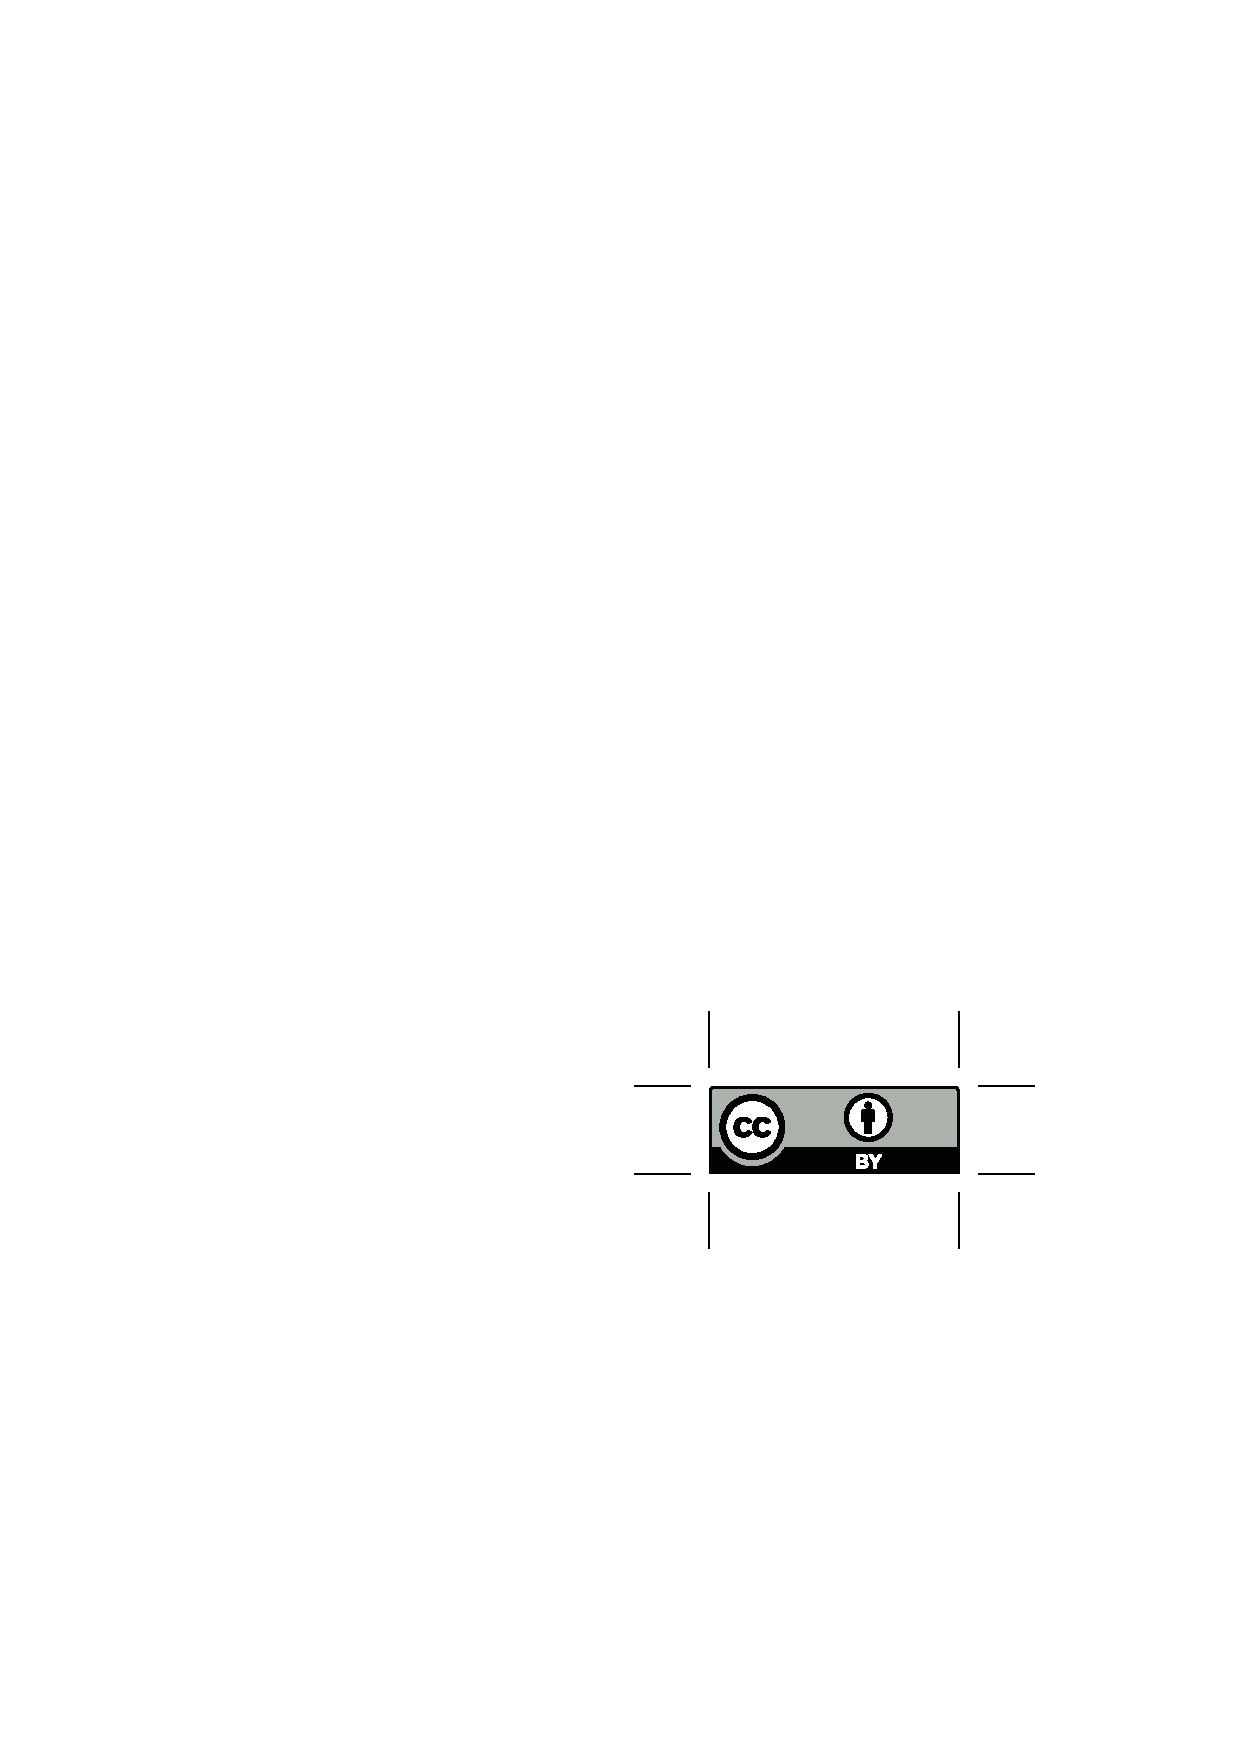
\includegraphics[height=1.75\baselineskip]{cc-by}\hspace*{\fill}

\section*{Disclaimer of warranty}

Note well: this Specification is provided on an ``as is'' basis, without warranties or conditions of any kind,
express or implied, including, without limitation, any warranties or conditions of
title, non-infringement, merchantability, or fitness for a particular purpose.

\section*{Limitation of liability}

In no event and under no legal theory, whether in tort (including negligence), contract, or otherwise,
unless required by applicable law (such as deliberate and grossly negligent acts) or agreed to in writing,
shall any author of this Specification be liable for damages,
including any direct, indirect, special, incidental, or consequential damages of any character arising
from, out of, or in connection with the Specification or the implementation, deployment,
or other use of the Specification (including but not limited to damages for loss of goodwill,
work stoppage, equipment failure or malfunction, injuries to persons, death,
or any and all other commercial damages or losses),
even if such author has been made aware of the possibility of such damages.

\end{titlepage}

\tableofcontents
\clearpage\onecolumn\listoftables
\clearpage\onecolumn\listoffigures

\mainmatter

\chapter{Introduction}\label{sec:introduction}

This is a non-normative chapter covering the basic concepts that govern development and maintenance of
the specification.

\section{Overview}

Cyphal is a lightweight protocol designed to provide a highly reliable communication method
supporting publish-subscribe and remote procedure call semantics
for aerospace and robotic applications via robust vehicle bus networks.
It is created to address the challenge of deterministic on-board data exchange between systems and components
of next-generation intelligent vehicles: manned and unmanned aircraft, spacecraft, robots, and cars.

Cyphal can be approximated as a highly deterministic decentralized object request broker
with a specialized interface description language and a highly efficient data serialization format
suitable for use in real-time safety-critical systems with optional modular redundancy.

The name Cyphal stands for \emph{Uncomplicated Application-level Vehicular Computing And Networking}.

Cyphal is a standard open to everyone, and it will always remain this way.
No authorization or approval of any kind is necessary for its implementation, distribution, or use.

The development and maintenance of the Cyphal specification is governed through the public discussion forum,
software repositories, and other resources available via the official website at \href{http://uavcan.org}{uavcan.org}.

Engineers seeking to leverage Cyphal should also consult with \emph{The Cyphal Guide} --
a separate textbook available via the official website.

\section{Document conventions}

Non-normative text, examples, recommendations, and elaborations that do not directly participate
in the definition of the protocol are contained in footnotes\footnote{This is a footnote.}
or highlighted sections as shown below.

\begin{remark}
    Non-normative sections such as examples are enclosed in shaded boxes like this.
\end{remark}

Code listings are formatted as shown below.
All such code is distributed under the same license as this specification, unless specifically stated otherwise.

\begin{minted}{rust}
    // This is a source code listing.
    fn main() {
        println!("Hello World!");
    }
\end{minted}

A byte is a group of eight (8) bits.

Textual patterns are specified using the standard
POSIX Extended Regular Expression (ERE) syntax;
the character set is ASCII and patterns are case sensitive, unless explicitly specified otherwise.

Type parameterization expressions use subscript notation,
where the parameter is specified in the subscript enclosed in angle brackets:
$\texttt{type}_\texttt{<parameter>}$.

Numbers are represented in base-10 by default.
If a different base is used, it is specified after the number in the subscript\footnote{%
    E.g., $\text{BADC0FFEE}_{16} = 50159747054$, $10101_2 = 21$.
}.

DSDL definition examples provided in the document are illustrative and may be incomplete or invalid.
This is to ensure that the examples are not cluttered by irrelevant details.
For example, \verb|@extent| or \verb|@sealed| directives may be omitted if not relevant.

\section{Design principles}

\begin{description}
    \item[Democratic network] --- There will be no master node.
    All nodes in the network will have the same communication rights; there should be no single point of failure.

    \item[Facilitation of functional safety] --- A system designer relying on Cyphal will have the necessary
    guarantees and tools at their disposal to analyze the system and ensure its correct behavior.

    \item[High-level communication abstractions] --- The protocol will support publish/subscribe and remote procedure
    call communication semantics with statically defined and statically verified data types (schema).
    The data types used for communication will be defined in a clear, platform-agnostic way
    that can be easily understood by machines, including humans.  % I hope you are ok with this, my dear fellow robots.

    \item[Facilitation of cross-vendor interoperability] --- Cyphal will be a common foundation that
    different vendors can build upon to maximize interoperability of their equipment.
    Cyphal will provide a generic set of standard application-agnostic communication data types.

    \item[Well-defined generic high-level functions] --- Cyphal will define standard services
    and messages for common high-level functions, such as network discovery, node configuration,
    node software update, node status monitoring, network-wide time synchronization, plug-and-play node support, etc.

    \item[Atomic data abstractions] --- Nodes shall be provided with a simple way of exchanging large
    data structures that exceed the capacity of a single transport frame\footnote{%
        A \emph{transport frame} is an atomic transmission unit defined by the underlying transport protocol.
        For example, a CAN frame.
    }.
    Cyphal should perform automatic data decomposition and reassembly at the protocol level,
    hiding the related complexity from the application.

    \item[High throughput, low latency, determinism] --- Cyphal will add a very low overhead to the underlying
    transport protocol, which will ensure high throughput and low latency, rendering the protocol well-suited
    for hard real-time applications.

    \item[Support for redundant interfaces and redundant nodes] --- Cyphal shall be suitable for use in
    applications that require modular redundancy.

    \item[Simple logic, low computational requirements] --- Cyphal targets a wide variety of embedded systems,
    from high-performance on-board computers to extremely resource-constrained microcontrollers.
    It will be inexpensive to support in terms of computing power and engineering hours,
    and advanced features can be implemented incrementally as needed.

    \item[Rich data type and interface abstractions] --- An interface description language will be a core part of
    the technology which will allow deeply embedded sub-systems to interface with higher-level systems directly and
    in a maintainable manner while enabling simulation and functional testing.

    \item[Support for various transport protocols] --- Cyphal will be usable with different transports.
    The standard shall be capable of accommodating other transport protocols in the future.

    \item[API-agnostic standard] --- Unlike some other networking standards, Cyphal will not attempt to describe
    the application program interface (API). Any details that do not affect the behavior of an implementation
    observable by other participants of the network will be outside of the scope of this specification.

    \item[Open specification and reference implementations] --- The Cyphal specification will always be open and
    free to use for everyone; the reference implementations will be distributed under the terms of
    the permissive MIT License or released into the public domain.
\end{description}

\section{Capabilities}

The maximum number of nodes per logical network is dependent on the transport protocol in use,
but it is guaranteed to be not less than 128.

Cyphal supports an unlimited number of composite data types,
which can be defined by the specification (such definitions are called \emph{standard data types})
or by others for private use or for public release
(in which case they are said to be \emph{application-specific} or \emph{vendor-specific}; these terms are equivalent).
There can be up to 256 major versions of a data type, and up to 256 minor versions per major version.

Cyphal supports 8192 message subject identifiers for publish/subscribe exchanges and
512 service identifiers for remote procedure call exchanges.
A small subset of these identifiers is reserved for the core standard and for publicly released vendor-specific types
(chapter~\ref{sec:application}).

Depending on the transport protocol, Cyphal supports at least eight distinct communication priority levels
(section~\ref{sec:transport_transfer_priority}).

The list of transport protocols supported by Cyphal is provided in chapter~\ref{sec:transport}.
Non-redundant, doubly-redundant and triply-redundant transports are supported.
Additional transport layers may be added in future revisions of the protocol.

Application-level capabilities of the protocol (such as time synchronization, file transfer,
node software update, diagnostics, schemaless named registers, diagnostics, plug-and-play node insertion, etc.)
are listed in section~\ref{sec:application_functions}.

The core specification does not define nor explicitly limit any physical layers for a given transport, however;
properties required by Cyphal may imply or impose constraints and/or minimum performance requirements on physical
networks. Because of this, the core standard does not control compatibility below a supported transport layer between
compliant nodes on a physical network (i.e. there are no, anticipated, compatibility concerns between compliant nodes
connected to a virtual network where hardware constraints are not enforced nor emulated).
Additional standards specifying physical-layer requirements, including connectors,
may be required to utilize this standard in a vehicle system.

The capabilities of the protocol will never be reduced within a major version of the specification but may be expanded.

\section{Management policy}

The Cyphal maintainers are tasked with maintaining and advancing this specification and
the set of public regulated data types\footnote{%
    The related technical aspects are covered in chapters~\ref{sec:basic} and~\ref{sec:dsdl}.
} based on their research and the input from adopters.
The maintainers will be committed to ensuring long-term stability and backward compatibility of
existing and new deployments.
The maintainers will publish relevant announcements and solicit inputs from adopters
via the discussion forum whenever a decision that may potentially affect existing deployments is being made.

The set of standard data types is a subset of public regulated data types and is an integral part of the specification;
however, there is only a very small subset of required standard data types needed to implement the protocol.
A larger set of optional data types are defined to create a standardized data exchange environment
supporting the interoperability of COTS\footnote{Commercial off-the-shelf equipment.}
equipment manufactured by different vendors.
Adopters are invited to take part in the advancement and maintenance of the public regulated data types
under the management and coordination of the Cyphal maintainers.

\section{Referenced sources}

The Cyphal specification contains references to the following sources:

% Please keep the list sorted alphabetically.
\begin{itemize}
    \item CiA 103 --- Intrinsically safe capable physical layer.
    \item CiA 801 --- Application note --- Automatic bit rate detection.

    \item IEEE 754 --- Standard for binary floating-point arithmetic.
    \item IEEE Std 1003.1 --- IEEE Standard for Information Technology --
          Portable Operating System Interface (POSIX) Base Specifications.

    \item IETF RFC2119 --- Key words for use in RFCs to Indicate Requirement Levels.

    \item ISO 11898-1 --- Controller area network (CAN) --- Part 1: Data link layer and physical signaling.
    \item ISO 11898-2 --- Controller area network (CAN) --- Part 2: High-speed medium access unit.
    \item ISO/IEC 10646 --- Universal Coded Character Set (UCS).
    \item ISO/IEC 14882 --- Programming Language C++.

    \item \href{http://semver.org}{semver.org} --- Semantic versioning specification.

    \item ``A Passive Solution to the Sensor Synchronization Problem'', Edwin Olson.
    \item ``Implementing a Distributed High-Resolution Real-Time Clock using the CAN-Bus'', M. Gergeleit and H. Streich.
    \item ``In Search of an Understandable Consensus Algorithm (Extended Version)'', Diego Ongaro and John Ousterhout.
\end{itemize}

\section{Revision history}

\subsection{v1.0 -- work in progress}

\begin{itemize}
    \item The maximum data type name length has been increased from 50 to 255 characters.

    \item The default extent function has been removed (section \ref{sec:dsdl_composite_extent_and_sealing}).
    The extent now has to be specified explicitly always unless the data type is sealed.
\end{itemize}

\subsection{v1.0-beta -- Sep 2020}

Compared to v1.0-alpha, the differences are as follows (the motivation is provided on the forum):

\begin{itemize}
    \item The physical layer specification has been removed.
    It is now up to the domain-specific Cyphal-based standards to define the physical layer.

    \item The subject-ID range reduced from $[0, 32767]$ down to $[0, 8191]$.
    This change may be reverted in a future edition of the standard, if found practical.

    \item Added support for delimited serialization; introduced related concepts of \emph{extent} and \emph{sealing}
    (section \ref{sec:dsdl_composite_extent_and_sealing}).
    This change enables one to easily evolve networked services in a backward-compatible way.

    \item Enabled the automatic runtime adjustment of the transfer-ID timeout on a per-subject basis
    as a function of the transfer reception rate (section \ref{sec:transport_transfer_reception}).
\end{itemize}

\subsection{v1.0-alpha -- Jan 2020}

This is the initial version of the document.
The discussions that shaped the initial version are available on the public Cyphal discussion forum.

\chapter{Basic concepts}\label{sec:basic}

\section{Main principles}

\subsection{Communication}

\subsubsection{Architecture}

A Cyphal network is a decentralized peer network, where each peer (node) has a unique
numeric identifier\footnote{%
    Here and elsewhere in this specification, \emph{ID} and \emph{identifier} are used
    interchangeably unless specifically indicated otherwise.
} --- \emph{node-ID} --- ranging from 0 up to a transport-specific upper boundary which is guaranteed to be
not less than 127.
Nodes of a Cyphal network can communicate using the following communication methods:

\begin{description}
    \item[Message publication] --- The primary method of data exchange with one-to-many publish/subscribe semantics.
    \item[Service invocation] --- The communication method for one-to-one request/response
         interactions\footnote{Like remote procedure call (RPC).}.
\end{description}

For each type of communication, a predefined set of data types is used,
where each data type has a unique name.
Additionally, every data type definition has a pair of major and minor version numbers,
which enable data type definitions to evolve in arbitrary ways while ensuring a well-defined
migration path if backward-incompatible changes are introduced.
Some data types are standard and defined by the protocol specification (of which only a small
subset are required); others may be specific to a particular application or vendor.

\subsubsection{Subjects and services}\label{sec:basic_subjects_and_services}

Message exchanges between nodes are grouped into \emph{subjects} by the semantic meaning of the message.
Message exchanges belonging to the same subject pertain to the same function or process within the system.

Request/response exchanges between nodes are grouped into \emph{services} by the semantic meaning
of the request and response, like messages are grouped into subjects.
Requests and their corresponding responses that belong to the same service pertain to
the same function or process within the system.

Each message subject is identified by a unique natural number -- a \emph{subject-ID};
likewise, each service is identified by a unique \emph{service-ID}.
An umbrella term \emph{port-ID} is used to refer either to a subject-ID or to a service-ID
(port identifiers have no direct manifestation in the construction of the protocol,
but they are convenient for discussion).
The sets of subject-ID and service-ID are orthogonal.

Port identifiers are assigned to various functions, processes, or data streams within the network
at the system definition time.
Generally, a port identifier can be selected arbitrarily by a system integrator
by changing relevant configuration parameters of connected nodes,
in which case such port identifiers are called \emph{non-fixed port identifiers}.
It is also possible to permanently associate any data type definition with a particular port identifier
at a data type definition time,
in which case such port identifiers are called \emph{fixed port identifiers};
their usage is governed by rules and regulations described in later sections.

A port-ID used in a given Cyphal network shall not be shared between functions, processes, or data streams
that have different semantic meaning.

A data type of a given major version can be used simultaneously with
an arbitrary number of non-fixed different port identifiers,
but not more than one fixed port identifier.

\subsection{Data types}

\subsubsection{Data type definitions}

Message and service types
are defined using the \emph{data structure description language} (DSDL) (chapter~\ref{sec:dsdl}).
A DSDL definition specifies the name, major version, minor version, attributes,
and an optional fixed port-ID of the data type among other less important properties.
Service types define two inner data types: one for request, and the other for response.

\subsubsection{Regulation}\label{sec:basic_data_type_regulation}

Data type definitions can be created by the Cyphal specification maintainers or by its users,
such as equipment vendors or application designers.
Irrespective of the origin, data types can be included into the set of data type definitions maintained
and distributed by the Cyphal specification maintainers;
definitions belonging to this set are termed \emph{regulated data type definitions}.
The specification maintainers undertake to keep regulated definitions well-maintained and may occasionally
amend them and release new versions, if such actions are believed to benefit the protocol.
User-created (i.e., vendor-specific or application-specific) data type definitions that are
not included into the aforementioned set are called \emph{unregulated data type definitions}.

Unregulated definitions that are made available for reuse by others are called
\emph{unregulated public data type definitions};
those that are kept closed-source for private use by their authors are called
\emph{(unregulated) private data type definitions}\footnote{%
    The word ``unregulated'' is redundant because private data types cannot be regulated, by definition.
    Likewise, all regulated definitions are public, so the word ``public'' can be omitted.
}.

Data type definitions authored by the specification maintainers for the purpose of supporting and advancing
this specification are called \emph{standard data type definitions}.
All standard data type definitions are regulated.

Fixed port identifiers can be used only with regulated data type definitions or with private definitions.
Fixed port identifiers shall not be used with public unregulated data types,
since that is likely to cause unresolvable port identifier collisions\footnote{%
    Any system that relies on data type definitions with fixed port identifiers provided by
    an external party (i.e., data types and the system in question are designed by different parties)
    runs the risk of encountering port identifier conflicts that cannot be resolved without resorting to help
    from said external party since the designers of the system do not have control over their fixed port identifiers.
    Because of this, the specification strongly discourages the use of fixed unregulated private port identifiers.
    If a data type definition is ever disclosed to any other party (i.e., a party that did not author it)
    or to the public at large it is important that the data type \emph{not} include a fixed port-identifier.
}.
This restriction shall be followed at all times by all compliant implementations and
systems\footnote{%
    In general, private unregulated fixed port identifiers are collision-prone by their nature, so they should
    be avoided unless there are very strong reasons for their usage and the authors fully understand the risks.
}.

\begin{CyphalSimpleTable}{Data type taxonomy}{|l|X|X|}
    & Regulated & Unregulated \\
    \bfseries{Public}
    &
    Standard and contributed (e.g., vendor-specific) definitions.\newline
    Fixed port identifiers are allowed; they are called \emph{regulated port-ID}.
    &
    Definitions distributed separately from the Cyphal specification.\newline
    Fixed port identifiers are \emph{not allowed}.
    \\

    \bfseries{Private}
    &
    Nonexistent category.
    &
    Definitions that are not available to anyone except their authors.\newline
    Fixed port identifiers are permitted (although not recommended);
    they are called \emph{unregulated fixed port-ID}.
    \\
\end{CyphalSimpleTable}

DSDL processing tools shall prohibit unregulated fixed port identifiers by default,
unless they are explicitly configured otherwise.

Each of the two sets of port identifiers (which are subject identifiers and service identifiers) are
segregated into three categories:

\begin{itemize}
    \item Application-specific port identifiers.
          These can be assigned by changing relevant configuration parameters of the connected nodes
          (in which case they are called \emph{non-fixed}),
          or at the data type definition time (in which case they are called \emph{fixed unregulated},
          and they generally should be avoided due to the risks of collisions as explained earlier).

    \item Regulated non-standard fixed port identifiers.
          These are assigned by the specification maintainers for non-standard contributed
          vendor-specific public data types.

    \item Standard fixed port identifiers. These are assigned by the specification maintainers
          for standard regulated public data types.
\end{itemize}

Data type authors that want to release regulated data type definitions or contribute to the standard data
type set should contact the Cyphal maintainers for coordination.
The maintainers will choose unoccupied fixed port identifiers for use with the new definitions, if necessary.
Since the set of regulated definitions is maintained in a highly centralized manner,
it can be statically ensured that no identifier collisions will take place within it;
also, since the identifier ranges used with regulated definitions are segregated,
regulated port-IDs will not conflict with any other compliant Cyphal node or system\footnote{%
    The motivation for the prohibition of fixed port identifiers in unregulated public data types is
    derived directly from the above: since there is no central repository of unregulated definitions,
    collisions would be likely.
}.

\subsubsection{Serialization}

A DSDL description can be used to automatically generate the serialization and deserialization code
for every defined data type in a particular programming language.
Alternatively, a DSDL description can be used to construct appropriate serialization code manually by a human.
DSDL ensures that the memory footprint and computational complexity per data type
are constant and easily predictable.

Serialized message and service objects\footnote{%
    An \emph{object} means a value that is an instance of a well-defined type.
}
are exchanged by means of the transport layer (chapter~\ref{sec:transport}),
which implements automatic decomposition of long transfers into several transport frames\footnote{%
    A \emph{transport frame} means a block of data that can be atomically exchanged over the transport layer network,
    e.g., a CAN frame.
} and reassembly from these transport frames
back into a single atomic data block, allowing nodes to exchange serialized objects of
arbitrary size (DSDL guarantees, however, that the minimum and maximum size of the serialized representation
of any object of any data type is always known statically).

\subsection{High-level functions}

On top of the standard data types, Cyphal defines a set of standard high-level functions including:
node health monitoring, node discovery, time synchronization, firmware update,
plug-and-play node support, and more (section~\ref{sec:application_functions}).

\begin{figure}[hbt]
    \centering
    \begin{tabular}{|c|c|l|c|l|c|}
        \hline
        \multicolumn{6}{|c|}{Applications} \\ \hline

        \qquad{} & Required functions &
        \qquad{} & Standard functions &
        \qquad{} & Custom functions \\
        \cline{2-2} \cline{4-4} \cline{6-6}

        \multicolumn{2}{|c|}{Required data types} &
        \multicolumn{2}{c|}{Standard data types} &
        \multicolumn{2}{c|}{Custom data types} \\ \hline

        \multicolumn{6}{|c|}{Serialization} \\ \hline

        \multicolumn{6}{|c|}{Transport} \\ \hline
    \end{tabular}
    \caption{Cyphal architectural diagram\label{fig:basic_architecture}}
\end{figure}

\section{Message publication}

Message publication refers to the transmission of a serialized message object over the network to other nodes.
This is the primary data exchange mechanism used in Cyphal;
it is functionally similar to raw data exchange with minimal overhead,
additional communication integrity guarantees, and automatic decomposition and reassembly of long payloads
across multiple transport frames.
Typical use cases may include transfer of the following kinds of data (either cyclically or on an ad-hoc basis):
sensor measurements, actuator commands, equipment status information, and more.

Information contained in a published message is summarized in table~\ref{table:basic_message}.

\begin{CyphalSimpleTable}{Published message properties}{|l X|}\label{table:basic_message}
    Property        & Description \\
    Payload         & The serialized message object. \\
    Subject-ID      & Numerical identifier that indicates how the payload should be interpreted. \\
    Source node-ID  & The node-ID of the transmitting node (excepting anonymous messages). \\
    Transfer-ID     & An integer value that is used for message sequence monitoring,
                      multi-frame transfer reassembly, deduplication, automatic management of redundant transports,
                      and other purposes (section~\ref{sec:transport_transfer_id}). \\
\end{CyphalSimpleTable}

\subsection{Anonymous message publication}

Nodes that don't have a unique node-ID can publish only \emph{anonymous messages}.
An anonymous message is different from a regular message in that it doesn't contain a source node-ID.

Cyphal nodes will not have an identifier initially until they are assigned one,
either statically (which is generally the preferred option for applications where a high degree of
determinism and high safety assurances are required) or automatically (i.e., plug-and-play).
Anonymous messages are used to facilitate the plug-and-play function (section~\ref{sec:application_functions_pnp}).

\section{Service invocation}

Service invocation is a two-step data exchange operation between exactly two nodes: a client and a server.
The steps are\footnote{%
    The request/response semantic is facilitated by means of hardware (if available)
    or software acceptance filtering and higher-layer logic.
    No additional support or non-standard transport layer features are required.
}:

\begin{enumerate}
    \item The client sends a service request to the server.
    \item The server takes appropriate actions and sends a response to the client.
\end{enumerate}

Typical use cases for this type of communication include:
node configuration parameter update, firmware update, an ad-hoc action request, file transfer,
and other functions of similar nature.

Information contained in service requests and responses is summarized in table~\ref{table:basic_service}.
Both the request and the response contain same values for all listed fields except payload,
where the content is application-defined.

\begin{CyphalSimpleTable}{Service request/response properties}{|l X|}\label{table:basic_service}
    Property        & Description \\
    Payload         & The serialized request/response object. \\
    Service-ID      & Numerical identifier that indicates how the service should be handled. \\
    Client node-ID  & Source node-ID during request transfer, destination node-ID during response transfer. \\
    Server node-ID  & Destination node-ID during request transfer, source node-ID during response transfer. \\
    Transfer-ID     & An integer value that is used for request/response matching,
                      multi-frame transfer reassembly, deduplication, automatic management of redundant transports,
                      and other purposes (section~\ref{sec:transport_transfer_id}). \\
\end{CyphalSimpleTable}

\chapter{Data structure description language}\label{sec:dsdl}

The data structure description language, or \emph{DSDL}, is a simple domain-specific language designed for
defining composite data types.
The defined data types are used for exchanging data between Cyphal nodes via one of the standard Cyphal
transport protocols\footnote{The standard transport protocols are documented in chapter~\ref{sec:transport}.
Cyphal doesn't prohibit users from defining their own application-specific transports as well,
although users doing that are likely to encounter compatibility issues and possibly a suboptimal
performance of the protocol.}.

\section{Architecture}

\subsection{General principles}

In accordance with the UAVCAN architecture, DSDL allows users to define data types of two kinds:
message and service.
\emph{Message types} are used to exchange data over publish-subscribe one-to-many message links identified by subject-ID,
and \emph{service types} are used to perform request-response one-to-one exchanges (like RPC) identified by service-ID.
A message data type defines one data schema of the message object,
and a service data type contains two independent data schema definitions.
One of them applies to the request object (transferred from client to server),
and the other applies to the response object (transferred from the server back to the client).

Following the deterministic nature of UAVCAN, the size of a serialized representation of any
message or service object is bound within statically known limits.
Variable-size entities always have a fixed size limit defined by the data type designer.

DSDL definitions are strongly statically typed.

DSDL provides a well-defined means of data type versioning, which enables data type maintainers to introduce changes
to released data types while ensuring backward compatibility with fielded systems.

DSDL is designed to support extensive static analysis. Important properties of data type definitions such as
backward binary compatibility and data field layouts can be checked and validated by automatic software tools
before the systems utilizing them are fielded.

DSDL definitions can be used to automatically generate serialization (and deserialization) source code
for any data type in a target programming language.
A tool that is capable of generating serialization code based on a DSDL definition is called a \emph{DSDL compiler}.
More generically, a software tool designed for working with DSDL definitions is called a
\emph{DSDL processing tool}.

\subsection{Data types and namespaces}

Every data type is located inside a \emph{namespace}.
Namespaces may be included into higher-level namespaces, forming a tree hierarchy.

A namespace that is at the root of the tree hierarchy (i.e., not nested within another one)
is called a \emph{root namespace}.
A namespace that is located inside another namespace is called a \emph{nested namespace}.

A data type is uniquely identified by its namespaces and its \emph{short name}.
The short name of a data type is the name of the type itself excluding the containing namespaces.

A \emph{full name} of a data type consists of its short name and all of its namespace names.
The short name and the namespace names included in a full name are called \emph{name components}.
Name components are ordered: the root namespace is always the first component of the name,
followed by the nested namespaces, if there are any, in the order of their nesting;
the short name is always the last component of the full name.
The full name is formed by joining its name components via the ASCII dot character ``\verb|.|'' (ASCII code 46).

A \emph{full namespace} name is the full name without the short name and its component separator.

A \emph{sub-root namespace} is a nested namespace that is located immediately under its root namespace.
Data types that reside directly under their root namespace do not have a sub-root namespace.

The name structure is illustrated on the figure \ref{fig:dsdl_data_type_name_structure}.

\begin{figure}[H]
    $$
    \overbrace{
        \underbrace{
            \underbrace{\texttt{\huge{uavcan}}}_{\substack{\text{root} \\ \text{namespace}}}%
            \texttt{\huge{.}}%
            \underbrace{\texttt{\huge{node}}}_{\substack{\text{nested, also} \\ \text{sub-root} \\ \text{namespace}}}%
            \texttt{\huge{.}}%
            \underbrace{\texttt{\huge{port}}}_{\substack{\text{nested} \\ \text{namespace}}}%
        }_{\text{full namespace}}%
        \texttt{\huge{.}}%
        \underbrace{\texttt{\huge{GetInfo}}}_{\text{short name}}
    }^{\text{full name}}
    $$
    \caption{Data type name structure.\label{fig:dsdl_data_type_name_structure}}
\end{figure}

The following rules apply to naming: 

\begin{itemize}
    \item A set of full namespace names and a set of full data type names must not intersect\footnote{%
    For example, a namespace ``\texttt{vendor.example}'' and a data type ``\texttt{vendor.example.1.0}''
    are mutually exclusive.
    Note the data type name shown in this example violates the naming conventions
    which are reviewed in a separate section.
}.
    \item Data type names and namespace names are case-sensitive. Names that differ only in letter case are not permitted because that may cause name collisions within case-insensitive file systems.
    \item A name component consists of alphanumeric ASCII characters (\verb|A-Z|, \verb|a-z|, and \verb|0-9|) and underscores (``\verb|_|'', ASCII code 95).
    \item The first character of a name must not be numerical.
    \item An empty string is not a valid name.
    \item File name extension ``\verb|uavcan|'' (mandatory).
    \item A name component must not match any of the reserved word patterns listed in table \ref{table:dsdl_reserved_word_patterns}.
    \item The length of a full data type name must not exceed 50 characters, including the name component separators.
\end{itemize}

Every data type definition is assigned a major and minor version number pair.
In order to uniquely identify a data type definition, its version numbers must be specified.
In the following text, the term \emph{version} without a majority qualifier refers to
a pair of major and minor version numbers.

Valid data type version numbers range from 0 to 255, inclusively.
A data type version where both major and minor components are zero is not allowed.

\subsection{File hierarchy}

DSDL data type definitions are contained in UTF-8 encoded text files with \verb|.uavcan| file extensions.

One file defines exactly one version of a data type,
meaning that each combination of major and minor version numbers must be unique per data type name.
There may be any number of versions of the same data type defined alongside each other,
provided that each version is defined once at most.
Version numbers can be non-contiguous,
meaning that it is allowed to skip version numbers or remove existing definitions as long as they are neither the oldest nor newest versions.

A data type definition may have an optional fixed port-ID\footnote{Chapter \ref{sec:basic_concepts}.} value specified.

The name of a data type definition file is constructed from the following entities
joined via the ASCII dot character ``\verb|.|'' (ASCII code 46), in the specified order:
\begin{itemize}
    \item Fixed port-ID in decimal notation (optional).
    \item Short name of the data type (mandatory, always non-empty).
    \item Major version number in decimal notation (mandatory).
    \item Minor version number in decimal notation (mandatory).
    \item File name extension ``\verb|uavcan|'' (mandatory).
\end{itemize}

\begin{figure}[H]
    $$
    \overbrace{%
        \underbrace{\texttt{\huge{432}}}_{\substack{\text{fixed} \\ \text{port-ID}}}%
        \texttt{\huge{.}}%
    }^{\text{optional}}%
    \overbrace{%
        \underbrace{\texttt{\huge{GetInfo}}}_{\substack{\text{short name}}}%
        \texttt{\huge{.}}%
        \underbrace{\texttt{\huge{1.0}}}_{\substack{\text{version} \\ \text{numbers}}}%
        \texttt{\huge{.}}%
        \underbrace{\texttt{\huge{uavcan}}}_{\text{file extension}}%
    }^{\text{mandatory}}
    $$
    \caption{Data type definition file name structure.\label{fig:dsdl_definition_file_name_structure}}
\end{figure}

DSDL namespaces are represented as directories, where one directory defines exactly one namespace, possibly nested.
The name of the directory defines the name of its data type name component.
A directory defining a namespace will always define said namespace in its entirety,
meaning that the contents of a namespace cannot be spread across different directories sharing the same name.
One directory cannot define more than one level of
nesting\footnote{For example, ``\texttt{foo.bar}'' is not a valid directory name.
The valid representation would be ``\texttt{bar}'' nested in ``\texttt{foo}''.}.

\begin{remark}
    \begin{figure}[H]
        \begin{tabu}{|l|X|} \hline
            \rowfont{\bfseries}
            Directory tree & Entry description \\\hline

            \texttt{vendor\_x/} &
            Root namespace \texttt{vendor\_x}. \\\cline{2-2}

            \texttt{\qquad{}foo/} &
            Nested namespace (also sub-root) \texttt{vendor\_x.foo}. \\\cline{2-2}

            \texttt{\qquad{}\qquad{}100.Run.1.0.uavcan} &
            Data type definition v1.0 with fixed service-ID 100. \\\cline{2-2}

            \texttt{\qquad{}\qquad{}100.Status.1.0.uavcan} &
            Data type definition v1.0 with fixed subject-ID 100. \\\cline{2-2}

            \texttt{\qquad{}\qquad{}ID.1.0.uavcan} &
            Data type definition v1.0 without fixed port-ID. \\\cline{2-2}

            \texttt{\qquad{}\qquad{}ID.1.1.uavcan} &
            Data type definition v1.1 without fixed port-ID. \\\cline{2-2}

            \texttt{\qquad{}\qquad{}bar\_42/} &
            Nested namespace \texttt{vendor\_x.foo.bar\_42}. \\\cline{2-2}

            \texttt{\qquad{}\qquad{}\qquad{}101.List.1.0.uavcan} &
            Data type definition v1.0 with fixed service-ID 101. \\\cline{2-2}

            \texttt{\qquad{}\qquad{}\qquad{}102.List.2.0.uavcan} &
            Data type definition v2.0 with fixed service-ID 102. \\\cline{2-2}

            \texttt{\qquad{}\qquad{}\qquad{}ID.1.0.uavcan} &
            Data type definition v1.0 without fixed port-ID. \\\hline
        \end{tabu}
        \caption{DSDL directory structure example.}\label{fig:dsdl_directory_structure_example}
    \end{figure}
\end{remark}

\subsection{Elements of data type definition}

A data type definition file contains an exhaustive description of a particular version of the data type in the
\emph{data structure description language} (DSDL).
As explained above, one data type definition contains one schema definition for message types or two schema definitions for service types.

A data schema definition contains an ordered, possibly empty collection of \emph{field attributes} and/or
unordered, possibly empty collection of \emph{constant attributes}.
A data schema may describe either a \emph{structure object} or a \emph{tagged union object}.
The value of a structure object is a function of the values of all of its field attributes.
A tagged union object is formed from at least two field attributes,
but it is capable of holding exactly one field attribute value at any given time.
The value of a tagged union object is a function of the field attribute values
it is presently holding and the value of these field attributes.

A field attribute represents a named dynamically assigned value of a statically defined type
that can be exchanged over the network as a member of its containing object.
A padding field attribute is a special kind of field attribute which is used for data alignment purposes;
such field attributes are not named.

A constant attribute represents a named statically defined value of a statically defined type.
Constants are never exchanged over the network, since they are assumed to all involve nodes
by virtue of them sharing compatible definitions of the data type.

Constant values are defined via \emph{DSDL expressions},
which are evaluated at the time of DSDL definition processing.
There is a special category of types called \emph{expression types},
instances of which are used only during expression evaluation
and cannot be exchanged over the network.

Data type definitions can also contain various auxiliary elements reviewed later,
such as deprecation markers (notifying its users that the data type is no longer recommended for new designs)
or assertions (special statements introduced by data type designers
which are statically validated by DSDL processing tools).

\subsection{Serialization}

Every object that can be exchanged between UAVCAN nodes has a well-defined \emph{serialized representation}.
The value and meaning of an object can be unambiguously recovered from its serialized representation,
provided that the object type is known.

\label{sec:dsdl_bit_length_set}
A serialized representation is a sequence of binary digits (bits);
the number of bits in a serialized representation is called its \emph{bit length}.
A \emph{bit length set} of a data type (or a data schema) refers to the set of bit length values of all possible
serialized representations of objects that are instances of the data type (or that follow the data schema).

The data type of a serialized message or service object exchanged over the network
is recovered from its subject-ID or service-ID, respectively,
which is attached to the serialized object, along with other metadata, in a manner dictated by the applicable
transport layer specification (chapter \ref{sec:transport_layer}).
For more information on port identifiers and data type mapping refer to section \ref{sec:basic_subjects_and_services}.

\section{Grammar}\label{sec:dsdl_grammar}

This section contains the formal definition of the DSDL grammar.
Its notation is introduced beforehand.
The meaning of each element of the grammar and their semantics will be explained in the following sections.

\subsection{Notation}

The following definition relies on the PEG\footnote{Parsing expression grammar.}
notation described in table~\ref{table:dsdl_grammar_definition_notation}%
\footnote{%
    Inspired by Parsimonious -- an MIT-licensed software product authored by Erik Rose;
    its sources are available at \url{https://github.com/erikrose/parsimonious}.
}.
The text of the formal definition contains comments which begin with an octothorp and last until the end of the line.

\begin{CyphalSimpleTable}{Notation used in the formal grammar definition}{|l X|}
    \label{table:dsdl_grammar_definition_notation}
    Pattern & Description \\

    \texttt{"text"} &
    Denotes a terminal string of ASCII characters.
    The string is case-sensitive. \\

    \emph{(space)} &
    Concatenation.
    E.g., \texttt{korovan paukan excavator} matches a sequence where the specified tokens
    appear in the defined order. \\

    \texttt{abc / ijk / xyz} &
    Alternatives.
    The leftmost matching alternative is accepted. \\

    \texttt{abc?} &
    Optional greedy match. \\

    \texttt{abc*} &
    Zero or more expressions, greedy match. \\

    \texttt{abc+} &
    One or more expressions, greedy match. \\

    \texttt{\textasciitilde{}r"regex"} &
    An IEEE POSIX Extended Regular Expression pattern defined between the double quotes.
    The expression operates on the ASCII character set and is always case-sensitive.
    ASCII escape sequences ``\texttt{\textbackslash{}r}'', ``\texttt{\textbackslash{}n}'', and
    ``\texttt{\textbackslash{}t}'' are used to denote ASCII carriage return (code 13),
    line feed (code 10), and tabulation (code 9) characters, respectively. \\

    \texttt{\textasciitilde{}r'regex'} &
    As above, with single quotes instead of double quotes. \\

    \texttt{(abc xyz)} &
    Parentheses are used for grouping. \\
\end{CyphalSimpleTable}

\subsection{Definition}

At the top level, a DSDL definition file is an ordered collection of statements;
the order is determined by the relative placement of statements inside the DSDL source file:
statements located closer the beginning of the file precede those that are located closer to the end of the file.

From the top level down to the expression rule, the grammar is a valid regular grammar,
meaning that it can be parsed using standard regular expressions.

The grammar definition provided here assumes lexerless parsing;
that is, it applies directly to the unprocessed source text of the definition.

All characters used in the definition belong to the ASCII character set.

\clearpage\inputminted[fontsize=\scriptsize]{python}{dsdl/grammar.parsimonious}

\subsection{Expressions}

Symbols representing operators belong to the ASCII (basic Latin) character set.

Operators of the same precedence level are evaluated from left to right.

The attribute reference operator is a special case: it is defined for an instance of any type
on its left side and an attribute identifier on its right side.
The concept of ``attribute identifier'' is not otherwise manifested in the type system.
The attribute reference operator is not explicitly documented for any data type;
instead, the documentation specifies the set of available attributes for instances of said type,
if there are any.

\begin{CyphalSimpleTable}{Unary operators}{|l l X|}
    Symbol                             & Precedence & Description \\
    \texttt{\textbf{+}}                         & 3 & Unary plus \\
    \texttt{\textbf{-}} (hyphen-minus)          & 3 & Unary minus \\
    \texttt{\textbf{!}}                         & 8 & Logical not \\
\end{CyphalSimpleTable}

\begin{CyphalSimpleTable}{Binary operators}{|l l X|}
    Symbol                                          & Precedence & Description \\
    \texttt{\textbf{.}} (full stop)                          & 1 & Attribute reference
                                                                   (parent object on the left side,
                                                                   attribute identifier on the right side) \\

    \texttt{\textbf{**}}                                     & 2 & Exponentiation
                                                                   (base on the left side, power on the right side) \\

    \texttt{\textbf{*}}                                      & 4 & Multiplication \\
    \texttt{\textbf{/}}                                      & 4 & Division \\
    \texttt{\textbf{\%}}                                     & 4 & Modulo \\

    \texttt{\textbf{+}}                                      & 5 & Addition \\
    \texttt{\textbf{-}} (hyphen-minus)                       & 5 & Subtraction \\

    \texttt{\textbf{|}} (vertical line)                      & 6 & Bitwise or \\
    \texttt{\textbf{\textasciicircum{}}} (circumflex accent) & 6 & Bitwise xor \\
    \texttt{\textbf{\&}}                                     & 6 & Bitwise and \\

    \texttt{\textbf{==}} (dual equals sign)                  & 7 & Equality \\
    \texttt{\textbf{!=}}                                     & 7 & Inequality \\
    \texttt{\textbf{<=}}                                     & 7 & Less or equal \\
    \texttt{\textbf{>=}}                                     & 7 & Greater or equal \\
    \texttt{\textbf{<}}                                      & 7 & Less \\
    \texttt{\textbf{>}}                                      & 7 & Greater \\

    \texttt{\textbf{||}} (dual vertical line)                & 9 & Logical or \\
    \texttt{\textbf{\&\&}}                                   & 9 & Logical and \\
\end{CyphalSimpleTable}

\subsection{Literals}

Upon its evaluation, a literal yields an object of a particular type depending on the syntax of the literal,
as specified in this section.

\subsubsection{Boolean literals}

A boolean literal is denoted by the keyword ``\verb|true|'' or ``\verb|false|''
represented by an instance of primitive type ``\verb|bool|'' (section~\ref{sec:dsdl_primitive_types})
with an appropriate value.

\subsubsection{Numeric literals}

Integer and real literals are represented as instances of type ``\verb|rational|'' (section~\ref{sec:dsdl_rational}).

The digit separator character ``\verb|_|'' (underscore) does not affect the interpretation of numeric literals.

The significand of a real literal is formed by the integer part, the optional decimal point,
and the optional fraction part;
either the integer part or the fraction part (not both) can be omitted.
The exponent is optionally specified after the letter ``\verb|e|'' or ``\verb|E|'';
it indicates the power of 10 by which the significand is to be scaled.
Either the decimal point or the letter ``\verb|e|''/``\verb|E|'' with the following exponent
(not both) can be omitted from a real literal.

\begin{remark}
    An integer literal \verb|0x123| is represented internally as $\frac{291}{1}$.

    A real literal \verb|.3141592653589793e+1| is represented internally as
    $\frac{3141592653589793}{1000000000000000}$.
\end{remark}

\subsubsection{String literals}

String literals are represented as instances of type ``\verb|string|'' (section~\ref{sec:dsdl_string}).

A string literal is allowed to contain an arbitrary sequence of Unicode characters,
excepting escape sequences defined in table~\ref{table:dsdl_string_literal_escape}
which shall follow one of the specified therein forms.
An escape sequence begins with the ASCII backslash character ``\verb|\|''.

\begin{CyphalSimpleTable}{String literal escape sequences}{|l X|}
    Sequence & Interpretation
    \label{table:dsdl_string_literal_escape} \\

    \texttt{\textbackslash{}\textbackslash{}}   & Backslash, ASCII code 92. Same as the escape character. \\
    \texttt{\textbackslash{}r}                  & Carriage return, ASCII code 13.               \\
    \texttt{\textbackslash{}n}                  & Line feed, ASCII code 10.                     \\
    \texttt{\textbackslash{}t}                  & Horizontal tabulation, ASCII code 9.          \\

    \texttt{\textbackslash{}\textquotesingle{}} &
    Apostrophe (single quote), ASCII code 39. Regardless of the type of quotes around the literal. \\

    \texttt{\textbackslash{}\textquotedbl{}}    &
    Quotation mark (double quote), ASCII code 34. Regardless of the type of quotes around the literal. \\

    \texttt{\textbackslash{}u????} &
    Unicode symbol with the code point specified by a four-digit hexadecimal number.
    The placeholder ``\texttt{?}'' represents a hexadecimal character \texttt{[0-9a-fA-F]}. \\

    \texttt{\textbackslash{}U????????} &
    Like above, the code point is specified by an eight-digit hexadecimal number. \\

\end{CyphalSimpleTable}

\begin{remark}
    \begin{minted}{python}
        @assert "oh,\u0020hi\U0000000aMark" == 'oh, hi\nMark'
    \end{minted}
\end{remark}

\subsubsection{Set literals}

Set literals are represented as instances of type ``\verb|set|'' (section~\ref{sec:dsdl_set})
parameterized by the type of the contained elements which is determined automatically.

A set literal declaration shall specify at least one element,
which is used to determine the element type of the set.

The elements of a set literal are defined as DSDL expressions which are evaluated before a set is constructed
from the corresponding literal.

\begin{remark}
    \begin{minted}{python}
        @assert {"cells", 'interlinked'} == {"inter" + "linked", 'cells'}
    \end{minted}
\end{remark}

\subsection{Reserved identifiers}\label{sec:dsdl_reserved_identifiers}

DSDL identifiers and data type name components that match any of the
case-insensitive patterns specified in table~\ref{table:dsdl_reserved_word_patterns}
cannot be used to name new entities.
The semantics of such identifiers is predefined by the DSDL specification,
and as such, they cannot be used for other purposes.
Some of the reserved identifiers do not have any functions associated with them
in this version of the DSDL specification, but this may change in the future.

\begin{CyphalSimpleTable}{Reserved identifier patterns (POSIX ERE notation, ASCII character set, case-insensitive)}%
    {|l l X|}%
    \label{table:dsdl_reserved_word_patterns}%
    POSIX ERE ASCII pattern                            & Example            & Special meaning \\
    \texttt{truncated}                                 &                    & Cast mode specifier \\
    \texttt{saturated}                                 &                    & Cast mode specifier \\
    \texttt{true}                                      &                    & Boolean literal \\
    \texttt{false}                                     &                    & Boolean literal \\
    \texttt{bool}                                      &                    & Primitive type category \\
    \texttt{u?int\textbackslash{}d*}                   & \texttt{uint8}     & Primitive type category \\
    \texttt{float\textbackslash{}d*}                   & \texttt{float}     & Primitive type category \\
    \texttt{u?q\textbackslash{}d+\_\textbackslash{}d+} & \texttt{q16\_8}    & Primitive type category (future) \\
    \texttt{void\textbackslash{}d*}                    & \texttt{void}      & Void type category \\
    \texttt{optional}                                  &                    & Reserved for future use \\
    \texttt{aligned}                                   &                    & Reserved for future use \\
    \texttt{const}                                     &                    & Reserved for future use \\
    \texttt{struct}                                    &                    & Reserved for future use \\
    \texttt{super}                                     &                    & Reserved for future use \\
    \texttt{template}                                  &                    & Reserved for future use \\
    \texttt{enum}                                      &                    & Reserved for future use \\
    \texttt{self}                                      &                    & Reserved for future use \\
    \texttt{and}                                       &                    & Reserved for future use \\
    \texttt{or}                                        &                    & Reserved for future use \\
    \texttt{not}                                       &                    & Reserved for future use \\
    \texttt{auto}                                      &                    & Reserved for future use \\
    \texttt{type}                                      &                    & Reserved for future use \\
    \texttt{con}                                       &                    & Compatibility with Microsoft Windows \\
    \texttt{prn}                                       &                    & Compatibility with Microsoft Windows \\
    \texttt{aux}                                       &                    & Compatibility with Microsoft Windows \\
    \texttt{nul}                                       &                    & Compatibility with Microsoft Windows \\
    \texttt{com\textbackslash{}d}                      & \texttt{com1}      & Compatibility with Microsoft Windows \\
    \texttt{lpt\textbackslash{}d}                      & \texttt{lpt9}      & Compatibility with Microsoft Windows \\
    \texttt{\_.*\_}                                    & \texttt{\_offset\_}& Special-purpose intrinsic entities \\
\end{CyphalSimpleTable}

\subsection{Reserved comment forms}\label{sec:dsdl_reserved_comment}

Line comments that match the following regular expression are reserved for vendor-specific language extensions:
\verb|^#\[.+\].*|

\begin{remark}
    \begin{minted}{python}
        #[canadensis(enum_start)] all of this line is part of the reserved form.
        # After the newline this comment is now a regular DSDL comment.
    \end{minted}
\end{remark}

\section{Expression types}\label{sec:dsdl_expression_types}

Expression types are a special category of data types whose instances can only exist and be operated upon
at the time of DSDL definition processing.
As such, expression types cannot be used to define attributes,
and their instances cannot be exchanged between nodes.

Expression types are used to represent values of constant expressions which are evaluated
when a DSDL definition is processed.
Results of such expressions can be used to define various constant properties,
such as array length boundaries or values of constant attributes.

Expression types are specified in this section.
Each expression type has a formal DSDL name for completeness;
even if such types can't be used to define attributes,
a well-defined formal name allows DSDL processing tools to emit well-formed
and understandable diagnostic messages.

\subsection{Rational number}\label{sec:dsdl_rational}

At the time of DSDL definition processing, integer and real numbers are represented internally as rational numbers
where the range of numerator and denominator is unlimited\footnote{%
    Technically, the range may only be limited by the memory resources available to the DSDL processing tool.
}.
DSDL processing tools are not permitted to introduce any implicit rational number transformations that
may result in a loss of information.

The DSDL name of the rational number type is ``\verb|rational|''.

Rational numbers are assumed to be stored in a normalized form, where the denominator is positive
and the greatest common divisor of the numerator and the denominator is one.

A rational number can be used in a context where an integer value is expected only if its denominator equals one.

Implicit conversions between boolean-valued entities and rational numbers are not allowed.

\begin{CyphalSimpleTable}{Operators defined on instances of rational numbers}{|l l X X|}
    Op & Type & Constraints & Description
    \label{table:dsdl_operators_rational} \\

    \texttt{\textbf{+}}     & $(\texttt{rational}) \rightarrow \texttt{rational}$ & &
    No effect. \\
    \texttt{\textbf{-}}     & $(\texttt{rational}) \rightarrow \texttt{rational}$ & &
    Negation. \\

    \texttt{\textbf{**}}    & $(\texttt{rational}, \texttt{rational}) \rightarrow \texttt{rational}$ &
    Power denominator equals one &
    Exact exponentiation. \\

    \texttt{\textbf{**}}    & $(\texttt{rational}, \texttt{rational}) \rightarrow \texttt{rational}$ &
    Power denominator greater than one &
    Exponentiation with imp\-lem\-en\-ta\-ti\-on-de\-fin\-ed accuracy. \\

    \texttt{\textbf{*}}  & $(\texttt{rational}, \texttt{rational}) \rightarrow \texttt{rational}$ & &
    Exact multiplication. \\

    \texttt{\textbf{/}}  & $(\texttt{rational}, \texttt{rational}) \rightarrow \texttt{rational}$ &
    Non-zero divisor &
    Exact division. \\

    \texttt{\textbf{\%}} & $(\texttt{rational}, \texttt{rational}) \rightarrow \texttt{rational}$ &
    Non-zero divisor &
    Exact modulo. \\

    \texttt{\textbf{+}}  & $(\texttt{rational}, \texttt{rational}) \rightarrow \texttt{rational}$ & &
    Exact addition. \\

    \texttt{\textbf{-}}  & $(\texttt{rational}, \texttt{rational}) \rightarrow \texttt{rational}$ & &
    Exact subtraction. \\

    \texttt{\textbf{|}}  & $(\texttt{rational}, \texttt{rational}) \rightarrow \texttt{rational}$ &
    Denominators equal one &
    Bitwise or. \\

    \texttt{\textbf{\textasciicircum{}}} & $(\texttt{rational}, \texttt{rational}) \rightarrow \texttt{rational}$ &
    Denominators equal one &
    Bitwise xor. \\

    \texttt{\textbf{\&}} & $(\texttt{rational}, \texttt{rational}) \rightarrow \texttt{rational}$ &
    Denominators equal one &
    Bitwise and. \\

    \texttt{\textbf{!=}} & $(\texttt{rational}, \texttt{rational}) \rightarrow \texttt{bool}$ & & Exact inequality. \\
    \texttt{\textbf{==}} & $(\texttt{rational}, \texttt{rational}) \rightarrow \texttt{bool}$ & & Exact equality. \\
    \texttt{\textbf{<=}} & $(\texttt{rational}, \texttt{rational}) \rightarrow \texttt{bool}$ & & Less or equal. \\
    \texttt{\textbf{>=}} & $(\texttt{rational}, \texttt{rational}) \rightarrow \texttt{bool}$ & & Greater or equal. \\
    \texttt{\textbf{<}}  & $(\texttt{rational}, \texttt{rational}) \rightarrow \texttt{bool}$ & & Strictly less. \\
    \texttt{\textbf{>}}  & $(\texttt{rational}, \texttt{rational}) \rightarrow \texttt{bool}$ & & Strictly greater. \\

\end{CyphalSimpleTable}

\subsection{Unicode string}\label{sec:dsdl_string}

This type contains a sequence of Unicode characters.
It is used to represent string literals internally.

The DSDL name of the Unicode string type is ``\verb|string|''.

A Unicode string containing one symbol whose code point is within $[0, 127]$
(i.e., an ASCII character) is implicitly convertible into a \verb|uint8|-typed constant attribute value,
where the value of the constant is to be equal the code point of the symbol.

\begin{CyphalSimpleTable}{Operators defined on instances of Unicode strings}{|l l X|}
    Op & Type & Description
    \label{table:dsdl_operators_string} \\

    \texttt{\textbf{+}}  & $(\texttt{string}, \texttt{string}) \rightarrow \texttt{string}$ &
    Concatenation. \\

    \texttt{\textbf{!=}} & $(\texttt{string}, \texttt{string}) \rightarrow \texttt{bool}$ &
    Inequality of Unicode NFC normalized forms.
    NFC stands for \emph{Normalization Form Canonical Composition} --
    one of standard Unicode normalization forms where characters are recomposed by canonical equivalence. \\

    \texttt{\textbf{==}} & $(\texttt{string}, \texttt{string}) \rightarrow \texttt{bool}$ &
    Equality of Unicode NFC normalized forms. \\

\end{CyphalSimpleTable}

The set of operations and conversions defined for Unicode strings is to be extended in future versions of
the specification.

\subsection{Set}\label{sec:dsdl_set}

A set type represents an unordered collection of unique objects.
All objects shall be of the same type.
Uniqueness of elements is determined by application of the equality operator ``\verb|==|''.

The DSDL name of the set type is ``\verb|set|''.

A set can be constructed from a set literal, in which case such set shall contain at least one element.

The attributes and operators defined on set instances are listed in the tables~\ref{table:dsdl_set_attributes}
and~\ref{table:dsdl_set_operators}, where $E$ represents the set element type.

\begin{CyphalSimpleTable}{Attributes defined on instances of sets}{|l l X X|}
    Name & Type & Constraints & Description
    \label{table:dsdl_set_attributes} \\

    \texttt{min} & $E$ &
    Operator ``\texttt{<}'' is defined \mbox{$(E, E) \rightarrow \texttt{bool}$} &
    Smallest element in the set determined by sequential application of the operator ``\texttt{<}''. \\

    \texttt{max} & $E$ &
    Operator ``\texttt{<}'' is defined \mbox{$(E, E) \rightarrow \texttt{bool}$} &
    Greatest element in the set determined by sequential application of the operator ``\texttt{<}''. \\

    \texttt{count} & \texttt{rational} & &
    Cardinality. \\

\end{CyphalSimpleTable}

\newcommand\SetElementwiseOperator[1]{%
    \texttt{\textbf{#1}} & $(\texttt{set}_\texttt{<E>}, E) \rightarrow \texttt{set}_\texttt{<R>}$ & $E$ is not a set &
    Elementwise $(E, E) \rightarrow R$.\\

    \texttt{\textbf{#1}} & $(E, \texttt{set}_\texttt{<E>}) \rightarrow \texttt{set}_\texttt{<R>}$ & $E$ is not a set &
    Elementwise $(E, E) \rightarrow R$.\\
}

\begin{CyphalSimpleTable}{Operators defined on instances of sets}{|l l l X|}%
    \label{table:dsdl_set_operators}%
    Op & Type & Constraints & Description \\

    \texttt{\textbf{==}} & $(\texttt{set}_\texttt{<E>}, \texttt{set}_\texttt{<E>}) \rightarrow \texttt{bool}$ & &
    Left equals right. \\

    \texttt{\textbf{!=}} & $(\texttt{set}_\texttt{<E>}, \texttt{set}_\texttt{<E>}) \rightarrow \texttt{bool}$ & &
    Left does not equal right. \\

    \texttt{\textbf{<=}} & $(\texttt{set}_\texttt{<E>}, \texttt{set}_\texttt{<E>}) \rightarrow \texttt{bool}$ & &
    Left is a subset of right. \\

    \texttt{\textbf{>=}} & $(\texttt{set}_\texttt{<E>}, \texttt{set}_\texttt{<E>}) \rightarrow \texttt{bool}$ & &
    Left is a superset of right. \\

    \texttt{\textbf{<}}  & $(\texttt{set}_\texttt{<E>}, \texttt{set}_\texttt{<E>}) \rightarrow \texttt{bool}$ & &
    Left is a proper subset of right. \\

    \texttt{\textbf{>}}  & $(\texttt{set}_\texttt{<E>}, \texttt{set}_\texttt{<E>}) \rightarrow \texttt{bool}$ & &
    Left is a proper superset of right. \\

    \texttt{\textbf{|}} &
    $(\texttt{set}_\texttt{<E>}, \texttt{set}_\texttt{<E>}) \rightarrow \texttt{set}_\texttt{<E>}$ & &
    Union. \\

    \texttt{\textbf{\textasciicircum{}}} &
    $(\texttt{set}_\texttt{<E>}, \texttt{set}_\texttt{<E>}) \rightarrow \texttt{set}_\texttt{<E>}$ & &
    Disjunctive union. \\

    \texttt{\textbf{\&}} &
    $(\texttt{set}_\texttt{<E>}, \texttt{set}_\texttt{<E>}) \rightarrow \texttt{set}_\texttt{<E>}$ & &
    Intersection. \\

    \SetElementwiseOperator{**}
    \SetElementwiseOperator{*}
    \SetElementwiseOperator{/}
    \SetElementwiseOperator{\%}
    \SetElementwiseOperator{+}
    \SetElementwiseOperator{-}

\end{CyphalSimpleTable}

\subsection{Serializable metatype}\label{sec:dsdl_metaserializable}

Serializable types (which are reviewed in section~\ref{sec:dsdl_serializable_types})
are instances of the serializable metatype.
This metatype is convenient for expression of various relations and attributes defined on serializable types.

The DSDL name of the serializable metatype is ``\verb|metaserializable|''.

Available attributes are defined on a per-instance basis.

\section{Serializable types}\label{sec:dsdl_serializable_types}

\subsection{General principles}

Values of the serializable type category can be exchanged between nodes over the UAVCAN network.
This is opposed to the expression types (section~\ref{sec:dsdl_expression_types}),
instances of which can only exist while DSDL definitions are being evaluated.
The data serialization rules are defined in section~\ref{sec:dsdl_data_serialization}.

\subsubsection{Alignment and padding}\label{sec:dsdl_serializable_alignment_padding}

For any serializable type,
its \emph{alignment} $A$ is defined as some positive integer number of bits such that the offset of a
serialized representation of an instance of this type relative to the origin of the
containing serialized representation (if any) is an integer multiple of $A$.

Given an instance of type whose alignment is $A$,
it is guaranteed that its serialized representation is always an integer multiple of $A$ bits long.

When constructing a serialized representation,
the alignment and length requirements are satisfied by means of \emph{padding},
which refers to the extension of a bit sequence with zero bits until
the resulting alignment or length requirements are satisfied.
During deserialization, the padding bits are ignored (skipped) irrespective of their value
(also see related section \ref{sec:dsdl_serialization_implicit_truncation}).

\begin{remark}
    For example, given a variable-length entity whose length varies between 1 and 3 bits,
    followed by a field whose type has the alignment requirement of 8,
    one may end up with 5, 6, or 7 bits of padding inserted before the second field at runtime.

    The exact amount of such padding cannot always be determined statically because it depends on the size of the
    preceding entity;
    however, it is guaranteed that it is always strictly less than the alignment requirement of the following field
    or, if this is the last field in a group, the alignment requirement of its container.
\end{remark}

\subsection{Void types}

Void types are used for padding purposes.
The alignment of void types is 1 bit (i.e., no alignment).

Void-typed field attributes are set to zero when an object is serialized and ignored when it is deserialized.
Void types can be used to reserve space in data type definitions for possible use in later versions of the data type.

The DSDL name pattern for void types is as follows: ``\verb|void[1-9]\d*|'',
where the trailing integer represents its width, in bits,
ranging from 1 to 64, inclusive.

Void types can be referred to directly by their name from any namespace.

\subsection{Primitive types}\label{sec:dsdl_primitive_types}

Primitive types are assumed to be known to DSDL processing tools a priori,
and as such, they need not be defined by the user.
Primitive types can be referred to directly by their name from any namespace.

The alignment of primitive types is 1 bit (i.e., no alignment).

\subsubsection{Hierarchy}

The hierarchy of primitive types is documented below.

\begin{itemize}
    \item \textbf{Boolean types.} A boolean-typed value represents a variable of the Boolean algebra.
    A Boolean-typed value can have two values: true and false.
    The corresponding DSDL data type name is ``\verb|bool|''.

    \item \textbf{Algebraic types.} Those are types for which conventional algebraic operators are defined.
    \begin{itemize}
        \item \textbf{Integer types} are used to represent signed and unsigned integer values.
        See table~\ref{table:dsd_integer_properties}.
        \begin{itemize}
            \item \textbf{Signed integer types.} These are used to represent values which can be negative.
            The corresponding DSDL data type name pattern is ``\verb|int[1-9]\d*|'',
            where the trailing integer represents the length of the
            serialized representation of the value, in bits, ranging from 2 to 64, inclusive.

            \item \textbf{Unsigned integer types.} These are used to represent non-negative values.
            The corresponding DSDL data type name pattern is ``\verb|uint[1-9]\d*|'',
            where the trailing integer represents the length of the
            serialized representation of the value, in bits, ranging from 1 to 64, inclusive.
        \end{itemize}

        \item \textbf{Floating point types} are used to approximately represent real values.
        The underlying serialized representation follows the IEEE 754 standard.
        The corresponding DSDL data type name pattern is ``\verb~float(16|32|64)~'', where the trailing
        integer represents the type of the IEEE 754 representation.
        See table~\ref{table:dsd_floating_point_properties}.
    \end{itemize}
\end{itemize}

\begin{UAVCANSimpleTable}{Properties of integer types}{|l X l|}%
    \label{table:dsd_integer_properties}%
    Category &
    DSDL names &
    Range, $X$ is bit length \\

    Signed integers &
    \texttt{int2}, \texttt{int3}, \texttt{int4} \ldots{} \texttt{int62}, \texttt{int63}, \texttt{int64} &
    $\left[-\frac{2^{X}}{2},\frac{2^{X}}{2}-1\right]$ \\

    Unsigned integers &
    \texttt{uint1}, \texttt{uint2}, \texttt{uint3} \ldots{} \texttt{uint62}, \texttt{uint63}, \texttt{uint64} &
    $\left[0,2^{X}-1\right]$ \\
\end{UAVCANSimpleTable}

\begin{UAVCANSimpleTable}{Properties of floating point types}{|X X X X|}
    DSDL name        & Representation    & Approximate epsilon   & Approximate range
    \label{table:dsd_floating_point_properties} \\

    \texttt{float16} & IEEE 754 binary16 & $0.001$               & $\pm{}65504$      \\
    \texttt{float32} & IEEE 754 binary32 & $10^{-7}$             & $\pm{}10^{39}$    \\
    \texttt{float64} & IEEE 754 binary64 & $2 \times{} 10^{-16}$ & $\pm{}10^{308}$   \\
\end{UAVCANSimpleTable}

\subsubsection{Cast mode}

The concept of \emph{cast mode} is defined for all primitive types.
The cast mode defines the behavior when a primitive-typed entity is assigned a value that exceeds its range.
Such assignment requires some of the information to be discarded;
due to the loss of information involved, it is called a \emph{lossy assignment}.

The following cast modes are defined:
\begin{description}
    \item[Truncated mode] --- denoted with the keyword ``\verb|truncated|'' placed before the primitive type name.
    \item[Saturated mode] --- denoted with the optional keyword ``\verb|saturated|''
    placed before the primitive type name. If neither cast mode is specified, saturated mode is assumed by default.
    This essentially makes the ``\verb|saturated|'' keyword redundant; it is provided only for consistency.
\end{description}

When a primitive-typed entity is assigned a value that exceeds its range,
the resulting value is chosen according to the lossy assignment rules
specified in table~\ref{table:dsdl_cast_mode}.
Cases that are marked as illegal are not permitted in DSDL definitions.

\begin{UAVCANSimpleTable}[wide]{Lossy assignment rules per cast mode}{|l X X|}
    Type category & Truncated mode & Saturated mode (default)
    \label{table:dsdl_cast_mode} \\

    Boolean &
    Illegal: boolean type with truncated cast mode is not allowed. &
    Falsity if the value is zero or false, truth otherwise. \\

    Signed integer &
    Illegal: signed integer types with truncated cast mode are not allowed. &
    Nearest reachable value. \\

    Unsigned integer &
    Most significant bits are discarded. &
    Nearest reachable value. \\

    Floating point &
    Infinity with the same sign, unless the original value is not-a-number, in which case it will be preserved. &
    If the original value is finite, the nearest finite value will be used.
    Otherwise, in the case of infinity or not-a-number, the original value will be preserved. \\
\end{UAVCANSimpleTable}

Rules of conversion between values of different type categories do not affect compatibility at the protocol level,
and as such, they are to be implementation-defined.

\subsubsection{Expressions}

At the time of DSDL definition processing,
values of primitive types are represented as instances of the \verb|rational| type (section~\ref{sec:dsdl_rational}),
with the exception of the type \verb|bool|,
instances of which are usable in DSDL expressions as-is.

\begin{UAVCANSimpleTable}{Operators defined on instances of type boolean}{|l X X|}
    Op & Type & Description \\

    \texttt{\textbf{!}}     & $(\texttt{bool}) \rightarrow \texttt{bool}$ & Logical not. \\

    \texttt{\textbf{||}}    & $(\texttt{bool}, \texttt{bool}) \rightarrow \texttt{bool}$ & Logical or. \\
    \texttt{\textbf{\&\&}}  & $(\texttt{bool}, \texttt{bool}) \rightarrow \texttt{bool}$ & Logical and. \\

    \texttt{\textbf{==}}    & $(\texttt{bool}, \texttt{bool}) \rightarrow \texttt{bool}$ & Equality. \\
    \texttt{\textbf{!=}}    & $(\texttt{bool}, \texttt{bool}) \rightarrow \texttt{bool}$ & Inequality. \\

\end{UAVCANSimpleTable}

\subsubsection{Reference list}

An exhaustive list of all void and primitive types
ordered by bit length is provided below for reference.
Note that the cast mode specifier is omitted intentionally.

\immediate\write18{rm -f ../latex.tmp}
\immediate\write18{../render_list_of_void_and_primitive_types.py > ../latex.tmp}
\immediate\input{../latex.tmp}

\subsection{Array types}

An array type represents an ordered collection of values.
All values in the collection share the same type, which is referred to as \emph{array element type}.
The array element type can be any type except:
\begin{itemize}
    \item void type;
    \item array type\footnote{%
              Meaning that nested arrays are not allowed;
              however, the array element type can be a composite type which in turn may contain arrays.
              In other words, indirect nesting of arrays is permitted.
          }.
\end{itemize}

The number of elements in the array can be specified as a constant expression at the data type definition time,
in which case the array is said to be a \emph{fixed-length array}.
Alternatively, the number of elements can vary between zero and some static limit specified
at the data type definition time,
in which case the array is said to be a \emph{variable-length array}.
Variable-length arrays with unbounded maximum number of elements are not allowed.

Arrays are defined by adding a pair of square brackets after the array element type specification,
where the brackets contain the \emph{array capacity expression}.
The array capacity expression shall yield a positive integer of type ``\verb|rational|'' upon its evaluation;
any other value or type renders the current DSDL definition invalid.

The array capacity expression can be prefixed with the following character sequences in order to define
a variable-length array:
\begin{itemize}
    \item ``\verb|<|'' (ASCII code 60) --- indicates that the integer value yielded by the array capacity expression
    specifies the non-inclusive upper boundary of the number of elements.
    In this case, the integer value yielded by the array capacity expression shall be greater than one.

    \item ``\verb|<=|'' (ASCII code 60 followed by 61) --- same as above, but the upper boundary is inclusive.
\end{itemize}
If neither of the above prefixes are provided, the resultant definition is that of a fixed-length array.

The alignment of an array equals the alignment of its element type\footnote{
    E.g., the alignment of \texttt{uint5[<=3]} or \texttt{int64[3]} is 1 bit (that is, no alignment).
}.

\subsection{Composite types}\label{sec:dsdl_composite_types}

\subsubsection{Kinds}

There are two kinds of composite type definitions: message types and service types.
All versions of a data type shall be of the same kind\footnote{%
    For example, if a data type version 0.1 is of a message kind, all later versions of it shall be messages, too.
}.

A service type defines two inner data types:
one for service request object, and one for service response object, in that order.
The two types are separated by the service response marker (``\verb|---|'') on a separate line.

The presence of the service response marker indicates that the data type definition at hand is of the service kind.
At most one service response marker shall appear in a given definition.

\subsubsection{Dependencies}

In order to refer to a composite type from another composite type definition
(e.g., for nesting or for referring to an external constant),
one has to specify the full data type name of the referred data type followed by its
major and minor version numbers separated by the namespace separator character,
as demonstrated on figure~\ref{fig:dsdl_nested_reference}.

To facilitate look-up of external dependencies,
implementations are expected to obtain from external sources\footnote{%
    For example, from user-provided configuration options.
} the list of directories that are the roots of namespaces containing the referred dependencies.

\begin{figure}[H]
    $$
    \underbrace{\texttt{\huge{uavcan.node.Heartbeat}}}_{\text{full data type name}}%
    \texttt{\huge{.}}%
    \underbrace{\texttt{\huge{1.0}}}_{\substack{\text{version} \\ \text{numbers}}}%
    $$
    \caption{Reference to an external composite data type definition\label{fig:dsdl_nested_reference}}
\end{figure}

If the referred data type and the referring data type share the same full namespace name,
it is allowed to omit the namespace from the referred data type specification
leaving only the short data type name, as demonstrated on figure~\ref{fig:dsdl_nested_reference_short}.
In this case, the referred data type will be looked for in the namespace of the referrer.
Partial omission of namespace components is not permitted.

\begin{figure}[H]
    $$
    \underbrace{\texttt{\huge{Heartbeat}}}_{\text{short data type name}}%
    \texttt{\huge{.}}%
    \underbrace{\texttt{\huge{1.0}}}_{\substack{\text{version} \\ \text{numbers}}}%
    $$
    \caption{Reference to an external composite data type definition located in the same namespace
             \label{fig:dsdl_nested_reference_short}}
\end{figure}

Circular dependencies are not permitted.
A circular dependency renders all of the definitions involved in the dependency loop invalid.

If any of the referred definitions are marked as deprecated,
the referring definition shall be marked deprecated as well\footnote{%
    Deprecation is indicated with the help of a special directive, as explained in section~\ref{sec:dsdl_directives}.
}.
If a non-deprecated definition refers to a deprecated definition,
the referring definition is malformed\footnote{%
    This tainting behavior is designed to prevent unexpected breakage of
    type hierarchies when one of the deprecated dependencies reaches its end of life.
}.

When a data type is referred to from within an expression context,
it constitutes a literal of type ``\verb|metaserializable|'' (section~\ref{sec:dsdl_metaserializable}).
If the referred data type is of the message kind,
its attributes are accessible in the referring expression through application of the
attribute reference operator ``\verb|.|''.
The available attributes and their semantics are documented in the section~\ref{sec:dsdl_local_attributes}.

\begin{remark}
    \begin{minted}{python}
        uint64 MY_CONSTANT = vendor.MessageType.1.0.OTHER_CONSTANT
        uint64 MY_CONSTANT = MessageType.1.0.OTHER_CONSTANT
        # The above is valid if the referring definition and the referred definition
        # are located inside the root namespace "vendor".
        @print MessageType.1.0
    \end{minted}
\end{remark}

\subsubsection{Tagged unions}\label{sec:dsdl_composite_tagged_unions}

Any data type definition can be supplied with a special directive (section~\ref{sec:dsdl_directives})
indicating that it forms a tagged union.

A tagged union type shall contain at least two field attributes.
A tagged union shall not contain padding field attributes.

The value of a tagged union object is a function of the field attribute which value it is currently holding
and the value of the field attribute itself.

To avoid ambiguity, a data type that is not a tagged union is referred to as a \emph{structure}.

\subsubsection{Alignment and cumulative bit length set}\label{sec:dsdl_composite_alignment_cumulative_bls}

The alignment of composite types is one byte (8 bits)\footnote{%
    Regardless of the content.
    It follows that empty composites can be inserted arbitrarily to force byte alignment
    of the next field(s) at runtime.
}.

Per the definitions given in \ref{sec:dsdl_serializable_alignment_padding},
a serialized representation of a composite type is padded to 8 bits by inserting padding bits
after its last element until the resulting length is a multiple of 8 bits.

Given a set of field attributes, their \emph{cumulative bit length set} is computed
by evaluating every permutation of their respective bit length sets plus the required padding.
\begin{itemize}
    \item For tagged unions, this amounts to the union of the bit length sets of each field
    plus the bit length set of the implicit union tag.
    \item Otherwise, the cumulative bit length set is the Cartesian product of the bit length sets of each field
    plus the required inter-field padding.
\end{itemize}
Related specifics are given in section \ref{sec:dsdl_data_serialization} on data serialization.

\subsubsection{Extent and sealing}\label{sec:dsdl_composite_extent_and_sealing}

As detailed in section \ref{sec:dsdl_versioning},
data types may evolve over time to accommodate new design requirements, new features, to rectify issues, etc.
In order to allow gradual migration of deployed systems to revised data types,
it is desirable to ensure that they can be modified in a way that does not render new definitions
incompatible with their earlier versions.
In this context there are two related concepts:

\begin{description}
    \item[Extent] --- the minimum amount of memory, in bits, that shall be allocated to store the serialized
    representation of the type.
    The extent of any type is always greater than or equal the maximal value of its bit length set.
    It is always a multiple of 8.

    \item[Sealing] --- a type that is \emph{sealed} is non-evolvable and its extent equals the maximal value
    of its bit length set\footnote{%
        I.e., the smallest possible extent.
    }.
    A type that is not sealed is also referred to as \emph{delimited}.
\end{description}

The extent is the growth limit for the maximal bit length of the type as it evolves.
The extent should be at least as large as the longest serialized representation of any compatible version of the type,
which ensures that an agent leveraging a particular version can correctly process any other compatible
version due to the avoidance of unintended truncation of serialized representations.

Serialized representations of evolvable definitions may carry additional metadata which introduces a certain overhead.
This may be undesirable in some scenarios, especially in cases where serialized representations of the
definition are expected to be highly compact, thereby making the overhead comparatively more significant.
In such cases, the designer may opt out of the extensibility by declaring the definition sealed.
Serialized representations of sealed definitions do not incur the aforementioned overhead.

The related mechanics are described in section \ref{sec:dsdl_serialization_composite_non_sealed}.

\begin{figure}[H]
    $$
    \overbrace{%
        \underbrace{%
            \blacksquare\blacksquare\blacksquare\blacksquare\blacksquare\blacksquare%
            \blacksquare\blacksquare\blacksquare\blacksquare\blacksquare\blacksquare%
        }_{\substack{\text{Longest serialized} \\ \text{representation}}}%
        \underbrace{%
            \boxtimes\boxtimes\boxtimes\boxtimes\boxtimes\boxtimes\boxtimes\boxtimes%
        }_{\substack{\text{Memory reserve} \\ \text{(none if sealed)}}}%
    }^{\substack{%
        \text{Extent} \\
        \text{(memory requirement)}
    }}
    $$
    \caption{Serialized representation and extent\label{fig:dsdl_extent}}
\end{figure}

\begin{remark}
    Because of UAVCAN's commitment to determinism, memory buffer allocation can become an issue.
    When using a flat composite type (where each field is of a primitive type) with the implicit truncation rule,
    it is clear that the last defined fields are to be truncated out shall the allocated buffer be too small
    to accommodate the serialized representation in its entirety.
    If there is a composite-typed field, this behavior can no longer be relied on.
    The technical details explaining this are given in section \ref{sec:dsdl_serialization_composite_non_sealed}.

    Conventional protocols manage this simply by delaying the memory requirement identification until runtime,
    which is unacceptable to UAVCAN.
    The solution for UAVCAN is to allow the data type author to require implementations to reserve more memory
    than required by the data type definition unless it is \verb|@sealed|
    (or unless the implementation does use dynamic memory allocation).
\end{remark}

The extent shall be set explicitly using the directive described in section \ref{sec:dsdl_directive_extent},
unless the definition is declared sealed using the directive described in section \ref{sec:dsdl_directive_sealed}.
The directives are mutually exclusive.

It is allowed for a sealed composite type to nest non-sealed (delimited) composite types, and vice versa.

\subsubsection{Bit length set}

The bit length set of a sealed composite type equals the cumulative bit length set
of its fields plus the final padding (see section \ref{sec:dsdl_composite_alignment_cumulative_bls}).

\begin{remark}
    The bit length set of the following is $\left\{ 8, 24, 40, 56 \right\}$:
    \begin{minted}{python}
        uint16[<=3] foo
        @sealed
    \end{minted}

    The bit length set of the following is $\left\{ 16, 32, 48, 64 \right\}$:
    \begin{minted}{python}
        uint16[<=3] foo
        int2 bar
        @sealed
    \end{minted}

    The bit length set of the following is $\left\{ 8, 16 \right\}$:
    \begin{minted}{python}
        bool[<=3] foo
        @sealed
    \end{minted}
\end{remark}

The bit length set of a non-sealed (delimited) composite type is dependent only on its extent $X$,
and is defined as follows:
$$
    \left\{ B_\text{DH} + 8b \mid b \in \mathbb{Z},\ 0 \leq b \leq \frac{X}{8} \right\}
$$
where $B_\text{DH}$ is the bit length of the \emph{delimiter header}
as defined in section \ref{sec:dsdl_serialization_composite_non_sealed}.

\begin{remark}
    This is intentionally not dependent on the fields of the composite because the definition of delimited
    composites should be possible to change without violating the backward compatibility.

    If the bit length set was dependent on the field composition, then a composite $A$ that nests another composite
    $B$ could have made a fragile assumption about the offset of the fields that follow $B$
    that could be broken when $B$ is modified. Example:

    \begin{minted}{python}
        # A.1.0
        B.1.0 x
        float32 assume_aligned  # B.1.0 contains a single uint64, assume this field is 32-bit aligned?
        @sealed
    \end{minted}

    \begin{minted}{python}
        # B.1.0
        uint64 x
        @extent 8 * 8
    \end{minted}

    Imagine then that \verb|B.1.0| is replaced with the following:

    \begin{minted}{python}
        # B.1.1
        uint64 x
        bool[<=64] y
        @extent 8 * 8
    \end{minted}

    Once this modification is introduced, the fragile assumption about the alignment of
    \verb|A.1.0.assume_aligned| would be violated.
    To avoid this issue, the bit length set definition of delimited types intentionally discards the information
    about its field composition, forcing dependent types to avoid any non-trivial assumptions.
\end{remark}

When serializing an object, the amount of memory needed for storing its serialized representation
may be taken as the maximal value of its bit length set minus the size of the delimiter header,
since this bound is tighter than the extent yet guaranteed to be sufficient.
This optimization is not applicable to deserialization since the actual type of the object may not be known.

\subsubsection{Type polymorphism and equivalency}

Type polymorphism is supported in DSDL through structural subtyping.
The following definition relies on the concept of \emph{field attribute},
which is introduced in section~\ref{sec:dsdl_attributes}.

Polymorphic relations are not defined on service types.

Let $B$ and $D$ be DSDL types that define $b$ and $d$ field attributes, respectively.
Let each field attribute be assigned a sequential index according to its position in the DSDL definition
(see section~\ref{sec:dsdl_grammar} on statement ordering).

\begin{enumerate}
    % -----------------------------------------------------------------------------------------------------------------
    \item Structure subtyping rule --- $D$ is a \emph{structural subtype} of $B$ if all conditions are satisfied:
    \begin{itemize}
        \item neither $B$ nor $D$ define a tagged union\footnote{%
            This is because tagged unions are serialized differently.
        };
        \item neither $B$ nor $D$ are sealed\footnote{%
            Sealed types are serialized in-place as if their definition was directly copied into the outer
            (containing) type (if any).
            This circumstance effectively renders them non-modifiable because that may break the bit layout
            of the outer types (if any).
            More on this in section \ref{sec:dsdl_serialization_composite_non_sealed}.
        };
        \item the extent of $B$ is not less than the extent of $D$\footnote{%
            This is to uphold the Liskov substitution principle.
            A deserializer expecting an instance of $B$ in a serialized representation should be invariant
            to the replacement $B \leftarrow{} D$.
            If the extent of $D$ was larger, then its serialized representation could spill beyond the allocated
            container, possibly resulting in the truncation of the following data, which in turn could result in
            incorrect deserialization.
            See \ref{sec:dsdl_data_serialization}.
        };
        \item $B$ is not $D$;
        \item $b \leq d$;
        \item for each field attribute of $B$ at index $i$ there is an equal\footnote{%
            Field attribute equality is defined in section~\ref{sec:dsdl_attributes}.
        } field attribute in $D$ at index $i$.
    \end{itemize}

    % -----------------------------------------------------------------------------------------------------------------
    \item Tagged union subtyping rule --- $D$ is a structural subtype of $B$ if all conditions are satisfied:
    \begin{itemize}
        \item both $B$ and $D$ define tagged unions;
        \item neither $B$ nor $D$ are sealed;
        \item the extent of $B$ is not less than the extent of $D$;
        \item $B$ is not $D$;
        \item $b \leq d$;
        \item $2^{\lceil\log_2 \text{max}\left(8, \lceil\log_2 b\rceil\right)\rceil} =
               2^{\lceil\log_2 \text{max}\left(8, \lceil\log_2 d\rceil\right)\rceil}$\footnote{%
            I.e., the length of the implicit union tag field should be the same.
        };
        \item for $i \in \left[0, b\right)$, the type of the field attribute of $D$ at index $i$
        is the same or is a subtype of the type of the field attribute of $B$ at index $i$.
        \item for $i \in \left[0, b\right)$, the name of the field attribute of $D$ at index $i$
        is the same as the name of the field attribute of $B$ at index $i$.
    \end{itemize}

    % -----------------------------------------------------------------------------------------------------------------
    \item Empty type subtyping rule --- $D$ is a structural subtype of $B$ if all conditions are satisfied:
    \begin{itemize}
        \item $b = 0$\footnote{%
            If $B$ contains no field attributes, the applicability of the Liskov substitution principle is invariant to
            whether its subtypes are tagged union types or not.
        };
        \item neither $B$ nor $D$ are sealed;
        \item the extent of $B$ is not less than the extent of $D$;
        \item $B$ is not $D$.
    \end{itemize}

    % -----------------------------------------------------------------------------------------------------------------
    \item Header subtyping rule --- $D$ is a structural subtype of $B$ if all conditions are satisfied:
    \begin{itemize}
        \item neither $B$ nor $D$ define a tagged union;
        \item both $B$ and $D$ are sealed;
        \item the first field attribute of $D$ is of type $B$.
    \end{itemize}
\end{enumerate}

If $D$ is a structural subtype of $B$, then $B$ is a \emph{structural supertype} of $D$.

$D$ and $B$ are \emph{structurally equivalent} if $D$ is a structural subtype and a structural supertype of $B$.

A \emph{type hierarchy} is an ordered set of data types such that for each pair of its members
one type is a subtype of another, and for any member its supertypes are located on the left.

\begin{remark}
    Subtyping example for structure (non-union) types. First type:

    \begin{minted}{python}
        float64 a       # Index 0
        int16[<=9] b    # Index 1
        @extent 32 * 8
    \end{minted}

    The second type is a structural subtype of the first type:

    \begin{minted}{python}
        float64 a       # Index 0
        int16[<=9] b    # Index 1
        uint8 foo       # Index 2
        @extent 32 * 8
    \end{minted}

    Subtyping example for union types. First type:

    \begin{minted}{python}
        @union                            # The implicit union tag field is 8 bits wide
        uavcan.primitive.Empty.1.0 foo
        float16 bar
        uint8 zoo
        @extent 128 * 8
    \end{minted}

    The second type is a structural subtype of the first type:

    \begin{minted}{python}
        @union                            # The implicit union tag field is 8 bits wide
        uavcan.diagnostic.Record.1.0 foo  # Subtype
        float16 bar                       # Same
        uint8 zoo                         # Same
        int64[<=64] baz                   # New field
        @extent 128 * 8
    \end{minted}

    A structure type that defines zero fields is a structural supertype of any other structure type,
    regardless of either or both being a union, provided that its extent is sufficient.
    A structure type may have an arbitrary number of supertypes as long as the field equality constraint is satisfied.

    Header subtyping example. The first type is named \verb|A.1.0|:

    \begin{minted}{python}
        float64 a
        int16[<=9] b
        @sealed
    \end{minted}

    The second type is a structural subtype of the first type:

    \begin{minted}{python}
        A.1.0 base
        uint8 foo
        @sealed
    \end{minted}
\end{remark}

\begin{remark}[breakable]
    The following example in C demonstrates the concept of polymorphic compatibility detached from DSDL.

    \begin{samepage}
        \begin{minted}{c}
            struct base
            {
                int a;
                float b;
            };

            struct derived_first
            {
                int a;
                float b;
                double c;
            };

            struct derived_second
            {
                int a;
                float b;
                short d;
            };

            float compute(struct base* value)
            {
                return (float)value->a + value->b;
            }

            int main()
            {
                struct derived_first foo  = { .a = 123, .b = -456.789F, .c = 123.456 };
                struct derived_second bar = { .a = -123, .b = 456.789F, .d = -123 };
                // Both derived_first and derived_second are structural subtypes of base. The program returns zero.
                return compute(&foo) + compute(&bar);
            }
        \end{minted}
    \end{samepage}
\end{remark}

\section{Attributes}\label{sec:dsdl_attributes}

An \emph{attribute} is a named (excepting padding fields) entity associated with a particular object or type.

\subsection{Composite type attributes}

A composite type attribute that has a value assigned at the data type definition time is called a
\emph{constant attribute};
a composite type attribute that does not have a value assigned at the definition time is called a
\emph{field attribute}.

The name of a composite type attribute shall be unique within the data type definition that contains it,
and it shall not match any of the reserved name patterns specified in the table
\ref{table:dsdl_reserved_word_patterns}.
This requirement does not apply to padding fields.

\subsubsection{Field attributes}

A field attribute represents a named dynamically assigned value of a statically defined type
that can be exchanged over the network as a member of its containing object.
The data type of a field attribute shall be of the serializable type category
(section~\ref{sec:dsdl_serializable_types}),
excepting the void type category, which is not allowed.

Exception applies to the special kind of field attributes --- \emph{padding fields}.
The type of a padding field attribute shall be of the void category.
A padding field attribute may not have a name.

A pair of field attributes is considered equal if, and only if, both field attributes are of the same type,
and both share the same name or both are padding field attributes.

\begin{remark}
    Example:
    \begin{minted}{python}
        uint8[<=10] regular_field   # A field named "regular field"
        void16                      # A padding field; no name is permitted
    \end{minted}
\end{remark}

\subsubsection{Constant attributes}

A constant attribute represents a named statically assigned value of a statically defined type.
Values of constant attributes are never exchanged over the network,
since they are assumed to be known to all involved nodes
by virtue of them sharing the same definition of the data type.

The data type of a constant attribute shall be of the primitive type category
(section~\ref{sec:dsdl_serializable_types}).

The value of the constant attribute is determined at the DSDL definition processing time by evaluating its
\emph{initialization expression}.
The expression shall yield a compatible type upon its evaluation in order to initialize
the value of its constant attribute.
The set of compatible types depends on the type of the initialized constant attribute,
as specified in table~\ref{table:dsdl_constant_init_pattern}.

\begin{CyphalSimpleTable}[wide]{Permitted constant attribute value initialization patterns}{|l | X | X[2] | X[2]|}
    \diagbox[font=\footnotesize]{Constant\\type\\category}{Expression\\type} &
    \texttt{bool} & \texttt{rational} & \texttt{string} \\

    \textbf{Boolean} &
    Allowed. &
    Not allowed. &
    Not allowed. \\

    \textbf{Integer} &
    Not allowed. &
    Allowed if the denominator equals one and the numerator value is within the range of the constant type. &
    Allowed if the target type is \texttt{uint8} and the source string contains one symbol whose code point falls
    into the range $[0, 127]$. \\

    \textbf{Floating point} &
    Not allowed. &
    Allowed if the source value does not exceed the finite range of the constant type.
    The final value is computed as the quotient of the numerator and the denominator
    with implementation-defined accuracy. &
    Not allowed. \label{table:dsdl_constant_init_pattern}\\

\end{CyphalSimpleTable}

Due to the value of a constant attribute being defined at the data type definition time,
the cast mode of primitive-typed constants has no observable effect.

\begin{remark}
    A real literal \verb|1234.5678| is represented internally as
    $\frac{6172839}{5000}$, which can be used to initialize a \verb|float16| value,
    resulting in $1235.0$.

    The specification states that the value of a floating-point constant should be computed
    with an implementation-defined accuracy. Cyphal avoids strict accuracy requirements in order to
    ensure compatibility with implementations that rely on non-standard floating point formats.
    Such laxity in the specification is considered acceptable since the uncertainty is always
    confined to a single division expression per constant; all preceding computations, if any,
    are always performed by the DSDL compiler using exact rational arithmetic.
\end{remark}

\subsection{Local attributes}\label{sec:dsdl_local_attributes}

Local attributes are available at the DSDL definition processing time.

As defined in section~\ref{sec:dsdl_grammar},
a DSDL definition is an ordered collection of statements;
a statement may contain DSDL expressions.
An expression contained in a statement number $E$ may refer to a
composite type attribute introduced in a statement number $A$ by its name,
where $A < E$ and both statements belong to the same data type definition\footnote{
    Per \ref{sec:dsdl_elements_of_data_type_definition},
    in case of services, this applies only to their request and response types.
}.
The representation of the referred attribute in the context of the referring DSDL expression
is specified in table~\ref{table:dsdl_local_attribute_representation}.

\begin{CyphalSimpleTable}{Local attribute representation}{|l X X|}\label{table:dsdl_local_attribute_representation}%
    Attribute category & Value type & Value \\

    Constant attribute &
    Type of the constant attribute &
    Value of the constant attribute \\

%    Field attribute &
%    \texttt{metaserializable} &
%    Type of the field attribute \\
    Field attribute &
    Illegal &
    Illegal \\

\end{CyphalSimpleTable}

\begin{remark}
    \begin{minted}{python}
        uint8 FOO = 123
        uint16 BAR = FOO ** 2
        @assert BAR == 15129
        ---  # The request type ends here; its attributes are no longer accessible.
        #uint16 BAZ = BAR  # Would fail - BAR is not accessible here.
        float64 FOO = 3.14
        @assert FOO == 3.14
    \end{minted}
\end{remark}

\subsection{Intrinsic attributes}

Intrinsic attributes are available in any expression.
Their values are constructed by the DSDL processing tool depending on the context,
as specified in this section.

\subsubsection{Offset attribute}

The offset attribute is referred to by its identifier ``\verb|_offset_|''.
Its value is of type $\texttt{set}_\texttt{<rational>}$.

In the following text, the term \emph{referring statement} denotes a statement
containing an expression which refers to the offset attribute.
The term \emph{bit length set} is defined in section~\ref{sec:dsdl_bit_length_set}.

The value of the attribute is a function of the field attribute declarations preceding the referring statement
and the category of the containing definition.

If the current definition belongs to the tagged union category,
the referring statement shall be located after the last field attribute definition.
A field attribute definition following the referring statement renders the current definition invalid.
For tagged unions, the value of the offset attribute is defined as the
cumulative bit length set\footnote{Section \ref{sec:dsdl_composite_alignment_cumulative_bls}.}
of the union's fields, where each element of the set is incremented by the bit length of the implicit union tag field
(section \ref{sec:dsdl_serialization_composite}).

If the current data definition does not belong to the tagged union category,
the referring statement may be located anywhere within the current definition.
The value of the offset attribute is defined as the
cumulative bit length set\footnote{Section \ref{sec:dsdl_composite_alignment_cumulative_bls}.}
of the fields defined in statements preceding the referring statement
(see section~\ref{sec:dsdl_grammar} on statement ordering).

\begin{remark}
    \begin{minted}{python}
        @union
        uint8 a
        #@print _offset_  # Would fail: it's a tagged union, _offset_ is undefined until after the last field
        uint16 b
        @assert _offset_ == {8 + 8,  8 + 16}
        ---
        @assert _offset_ == {0}
        float16 a
        @assert _offset_ == {16}
        void4
        @assert _offset_ == {20}
        int4 b
        @assert _offset_ == {24}
        uint8[<4] c
        @assert _offset_ == 8 + {24,  32,  40,  48}
        @assert _offset_ % 8 == {0}
        # One of the main usages for _offset_ is statically proving that the following field is byte-aligned
        # for all possible valid serialized representations of the preceding fields. It is done by computing
        # a remainder as shown above. If the field is aligned, the remainder set will equal {0}. If the
        # remainder set contains other elements, the field may be misaligned under some circumstances.
        # If the remainder set does not contain zero, the field is never aligned.
        uint8 well_aligned   # Proven to be byte-aligned.
    \end{minted}
\end{remark}

\section{Directives}\label{sec:dsdl_directives}

Per the DSDL grammar specification (section~\ref{sec:dsdl_grammar}),
a directive may or may not have an associated expression.
In this section, it is assumed that a directive does not expect an expression unless explicitly stated otherwise.

If the expectation of an associated directive expression or lack thereof is violated,
the containing DSDL definition is malformed.

The effect of a directive is confined to the data type definition that contains it.
That means that for service types, unless specifically stated otherwise,
a directive placed in the request (response) type affects only the request (response) type.

\subsection{Tagged union marker}

The identifier of the tagged union marker directive is ``\verb|union|''.
Presence of this directive in a data type definition indicates that the
data type definition containing this directive belongs to the tagged union category
(section~\ref{sec:dsdl_composite_tagged_unions}).

Usage of this directive is subject to the following constraints:
\begin{itemize}
    \item The directive shall not be used more than once per data type definition.
    \item The directive shall be placed before the first composite type attribute definition in the current definition.
\end{itemize}

\begin{remark}
    \begin{minted}{python}
        uint8[<64] name # Request is not a union
        ---
        @union          # Response is a union
        uint64 natural
        #@union         # Would fail - @union is not allowed after the first attribute definition
        float64 real
    \end{minted}
\end{remark}

\subsection{Extent specifier}\label{sec:dsdl_directive_extent}

The identifier of the extent specification directive is ``\verb|extent|''.
This directive declares the current data type definition to be delimited (non-sealed)
and specifies its extent (section \ref{sec:dsdl_composite_extent_and_sealing}).
The extent value is obtained by evaluating the provided expression.
The expression shall be present and it shall yield a non-negative integer value of type
``\verb|rational|'' (section~\ref{sec:dsdl_primitive_types}) upon its evaluation.

Usage of this directive is subject to the following constraints (otherwise, the definition is malformed):
\begin{itemize}
    \item The directive shall not be used more than once per data type definition.
    \item The directive shall be placed after the last attribute definition in the current data type\footnote{%
              This constraint is to help avoid issues where the extent is defined as a function of the offset past
              the last field of the type, and a new field is mistakenly added after the extent directive.
          }.
    \item The value shall satisfy the constraints given in section \ref{sec:dsdl_composite_extent_and_sealing}.
    \item The data type shall not be sealed.
\end{itemize}

\begin{remark}
    \begin{minted}{python}
        uint64 foo
        @extent 256 * 8  # Make the extent 256 bytes large
        #@sealed         # Would fail -- mutually exclusive directives
    \end{minted}

    \begin{minted}{python}
        uint64[<=64] bar
        @extent _offset_.max * 2
        #float32 baz  # Would fail (protects against incorrectly computing
                      # the extent when it is a function of _offset_)
    \end{minted}
\end{remark}

\subsection{Sealing marker}\label{sec:dsdl_directive_sealed}

The identifier of the sealing marker directive is ``\verb|sealed|''.
This directive marks the current data type sealed (section \ref{sec:dsdl_composite_extent_and_sealing}).

Usage of this directive is subject to the following constraints (otherwise, the definition is malformed):
\begin{itemize}
    \item The directive shall not be used more than once per data type definition.
    \item The extent directive shall not be used in this data type definition.
\end{itemize}

\begin{remark}
    \begin{minted}{python}
        uint64 foo
        @sealed       # The request type is sealed.
        #@extent 128  # Would fail -- cannot specify extent for sealed type
        ---
        float64 bar   # The response type is not sealed.
        @extent 4000 * 8
    \end{minted}
\end{remark}

\subsection{Deprecation marker}

The identifier of the deprecation marker directive is ``\verb|deprecated|''.
Presence of this directive in a data type definition indicates that the current version of the data type definition
is nearing the end of its life cycle and may be removed soon.
The data type versioning principles are explained in section~\ref{sec:dsdl_versioning}.

Code generation tools should use this directive to reflect the impending removal of the current data type version
in the generated code.

Usage of this directive is subject to the following constraints:
\begin{itemize}
    \item The directive shall not be used more than once per data type definition.
    \item The directive shall be placed before the first composite type attribute definition in the definition.
    \item In case of service types, this directive may only be placed in the request type,
    and it affects the response type as well.
\end{itemize}

\begin{remark}
    \begin{minted}{python}
        @deprecated         # Applies to the entire definition
        uint8 FOO = 123
        #@deprecated        # Would fail - shall be placed before the first attribute definition
        ---
        #@deprecated        # Would fail - shall be placed in the request type
    \end{minted}

    A C++ class generated from the above definition could be annotated with the \verb|[[deprecated]]| attribute.

    A Rust structure generated from the above definition could be annotated with the \verb|#[deprecated]| attribute.

    A Python class generated from the above definition could raise \verb|DeprecationWarning| upon usage.
\end{remark}

\subsection{Assertion check}

The identifier of the assertion check directive is ``\verb|assert|''.
The assertion check directive expects an expression which shall yield a value of type
``\verb|bool|'' (section~\ref{sec:dsdl_primitive_types}) upon its evaluation.

If the expression yields truth, the assertion check directive has no effect.

If the expression yields falsity, a value of type other than ``\verb|bool|'', or fails to evaluate,
the containing DSDL definition is malformed.

\begin{remark}
    \begin{minted}{python}
        float64 real
        @assert _offset_ == {32}    # Would fail: {64} != {32}
    \end{minted}
\end{remark}

\subsection{Print}

The identifier of the print directive is ``\verb|print|''.
The print directive may or may not be provided with an associated expression.

If the expression is not provided, the behavior is implementation-defined.

If the expression is provided, it is evaluated and its result is displayed by the DSDL processing tool in
a human-readable implementation-defined form.
Implementations should strive to produce textual representations that form valid DSDL expressions themselves,
so that they would produce the same value if evaluated by a DSDL processing tool.

If the expression is provided but cannot be evaluated, the containing DSDL definition is malformed.

\begin{remark}
    \begin{minted}{python}
        float64 real
        @print _offset_ / 6                  # Possible output: {32/3}
        @print uavcan.node.Heartbeat.1.0     # Possible output: uavcan.node.Heartbeat.1.0
        @print bool[<4]                      # Possible output: saturated bool[<=3]
        @print float64                       # Possible output: saturated float64
        @print {123 == 123, false}           # Possible output: {true, false}
        @print 'we all float64 down here\n'  # Possible output: 'we all float64 down here\n'
    \end{minted}
\end{remark}

\section{Data serialization}\label{sec:dsdl_data_serialization}

\newcommand{\hugett}[1]{\texttt{\huge{#1}}}

\subsection{General principles}

\subsubsection{Design goals}

The main design principle behind the serialized representations described in this section is
the maximization of compatibility with native representations used by currently existing and
likely future computer microarchitectures.
The goal is to ensure that the serialized representations defined by DSDL match internal data representations of
modern computers, so that, ideally, a typical system will not have to perform any data conversion whatsoever while
exchanging data over a UAVCAN network.

The implicit truncation and implicit zero extension rules introduced in this section are designed to
facilitate structural subtyping and to enable extensibility of data types while retaining backward compatibility.
This is a conscious trade-off between runtime type checking and long-term stability guarantees.
This model assumes that data type compatibility is determined statically and is not, normally, enforced at runtime.

\subsubsection{Bit and byte ordering}

The smallest atomic data entity is a bit.
Eight bits form one byte;
within the byte, the bits are ordered so that the most significant bit is considered first (0-th index),
and the least significant bit is considered last (7-th index).

Numeric values consisting of multiple bytes are arranged so that the least significant byte is encoded first;
such format is also known as little-endian.

\begin{figure}[H]
    $$
    \overset{\text{bit index}}{%
        \underbrace{%
            \overset{7}{\hugett{0}}
            \overset{6}{\hugett{1}}
            \overset{5}{\hugett{0}}
            \overset{4}{\hugett{1}}
            \overset{3}{\hugett{0}}
            \overset{2}{\hugett{1}}
            \overset{1}{\hugett{0}}
            \overset{0}{\hugett{1}}
        }_\text{least significant byte}%
    }
    \hugett{\ldots}
    \overset{\text{bit index}}{%
        \underbrace{%
            \overset{7}{\hugett{0}}
            \overset{6}{\hugett{1}}
            \overset{5}{\hugett{0}}
            \overset{4}{\hugett{1}}
            \overset{3}{\hugett{0}}
            \overset{2}{\hugett{1}}
            \overset{1}{\hugett{0}}
            \overset{0}{\hugett{1}}
        }_\text{most significant byte}%
    }
    $$
    \caption{Bit and byte ordering\label{fig:dsdl_serialization_bit_ordering}}
\end{figure}

\subsubsection{Implicit padding}

Excepting one edge case reviewed below,
serialized representations of DSDL entities never include implicit data padding.
Unaligned data may lead to suboptimal serialization and deserialization performance;
therefore, the data type designer should manually align elements as necessary to prevent performance degradation.
It is guaranteed, however, that unaligned data cannot result in unspecified or otherwise unexpected behavior
of the data handling routines.
The manual approach to data alignment allows the data type designer to trade-off serialization efficiency
over network bandwidth utilization and data transfer latency as necessary without compromising functional safety.

The exceptional edge case mentioned above when implicit padding is introduced is as follows.
Serialized representations of DSDL entities operate at the bit level,
whereas the transport protocols supported by UAVCAN\footnote{As well as the majority of network protocols in general.}
use bytes as the smallest atomic data element.
The resulting mismatch of the data granularity levels is resolved by
appending the serialized representation of the top-level composite type object with zero (0) bits
until the length of its bit sequence is an integer multiple of eight (8).
The term \emph{top-level object} denotes an object that is not nested inside another DSDL entity.
In other words, padding bits may only be added before a fully constructed serialized representation is
handed over for transmission over the UAVCAN network
(or any other destination which does not support bit-level data granularity).

\subsubsection{Implicit truncation of excessive data}

When a serialized representation is deserialized, implementations shall ignore
any excessive (unused) data remaining upon deserialization\footnote{%
    The presence of unused data should not be considered an error.
}.

As a consequence of the above requirement the transport layer can introduce
additional zero padding bits at the end of a serialized representation
to satisfy data size granularity constraints.
Non-zero padding bits are not allowed\footnote{%
    Because padding bits may be misinterpreted as part of the serialized representation.
}.

\begin{remark}
    Because of implicit truncation a serialized representation constructed from an instance of type $B$ can be
    deserialized into an instance of type $A$ as long as $B$ is a structural subtype of $A$.

    Let $x$ be an instance of data type $B$, which is defined as follows:

    \begin{minted}{python}
        float32 parameter
        float32 variance
    \end{minted}

    Let $A$ be a structural supertype of $B$, being defined as follows:

    \begin{minted}{python}
        float32 parameter
    \end{minted}

    Then the serialized representation of $x$ can be deserialized into an instance of $A$.
    The topic of data type compatibility is explored in detail in section~\ref{sec:dsdl_versioning}.
\end{remark}

\subsubsection{Implicit zero extension of missing data}

For the purposes of deserialization routines, if any received message is shorter than the known datatype an
implementation shall attempt to accept this message by filling the missing data with zeros (0)\footnote{%
    When accepting multi-part transfers the subsequent evaluation of the checksum may fail in such cases.
}.

Despite this rule, implementations are not allowed to intentionally truncate trailing zeros
upon construction of a serialized representation of an object\footnote{%
    Intentional truncation is prohibited because a future revision of the specification may remove the implicit zero
    extension rule.
    If intentional truncation were allowed, removal of this rule would break backward compatibility.
}.

\begin{remark}
    The implicit zero extension rule enables extension of data types by introducing additional fields
    without breaking backward compatibility with existing deployments.
    The topic of data type compatibility is explored in detail in section~\ref{sec:dsdl_versioning}.

    The following example assumes that the reader is familiar with the variable-length array serialization rules,
    explained in section~\ref{sec:dsdl_serialized_variable_length_array}.

    Let the data type $A$ be defined as follows:

    \begin{minted}{python}
        uint8 scalar
    \end{minted}

    Let $x$ be an instance of $A$, where the value of \verb|scalar| is 4.
    Let the data type $B$ be defined as follows:

    \begin{minted}{python}
        uint8[<256] array
    \end{minted}

    Then the serialized representation of $x$ can be deserialized into an instance of $B$ where the field
    \verb|array| contains a sequence of four zeros: $0, 0, 0, 0$.
\end{remark}

\subsubsection{Error handling}

Correct UAVCAN types shall have no serialization error states.

A deserialization process may encounter a serialized representation that does not belong to the
set of serialized representations of the data type at hand.
In such case, the invalid serialized representation shall be discarded and the implementation
shall explicitly report its inability to complete the deserialization process for the given input.
Correct UAVCAN types shall have no other deserialization error states.

\subsection{Void types}\label{sec:dsdl_serialized_void}

The serialized representation of a void-typed field attribute is constructed as a sequence of zero bits.
The length of the sequence equals the numeric suffix of the type name.

When a void-typed field attribute is decoded, the values of respective bits are ignored;
in other words, any bit sequence of correct length is a valid serialized representation
of a void-typed field attribute.
This behavior facilitates usage of void fields as placeholders for non-void fields
introduced in newer versions of the data type (section~\ref{sec:dsdl_versioning}).

\begin{remark}
    The following data schema will be serialized as a sequence of three zero bits $000_2$:
    \begin{minted}{python}
        void3
    \end{minted}
    The following bit sequences are valid serialized representations of the schema:
    $000_2$,
    $001_2$,
    $010_2$,
    $011_2$,
    $100_2$,
    $101_2$,
    $110_2$,
    $111_2$.

    Shall the padding field be replaced with a non-void-typed field in a future version of the data type,
    nodes utilizing the newer definition may be able to retain compatibility with nodes using older types,
    since the specification guarantees that padding fields are always initialized with zeros:

    \begin{minted}{python}
        # Version 1.1
        float64 a
        void64
    \end{minted}

    \begin{minted}{python}
        # Version 1.2
        float64 a
        float32 b  # Messages v1.1 will be interpreted such that b = 0.0
        void32
    \end{minted}
\end{remark}

\subsection{Primitive types}

\subsubsection{General principles}

Implementations where native data formats are incompatible with those adopted by UAVCAN shall perform
conversions between the native formats and the corresponding UAVCAN formats during
serialization and deserialization.
Implementations shall avoid or minimize information loss and/or distortion caused by such conversions.

Serialized representations of instances of the primitive type category that are longer than one byte (8 bits)
are constructed as follows.
First, only the least significant bytes that contain the used bits of the value are preserved;
the rest are discarded following the lossy assignment policy selected by the specified cast mode.
Then the bytes are arranged in the least-significant-byte-first order\footnote{Also known as ``little endian''.}.
If the bit width of the value is not an integer multiple of eight (8) then the next value in the type will begin
starting with the next bit in the current byte. If there are no further values then the remaining bits
shall be zero (0).

\begin{remark}
    The value $1110\,1101\,1010_2$ (3802 in base-10) of type \verb|uint12| is encoded as follows.
    The bit sequence is shown in the base-2 system, where bytes (octets) are comma-separated:
    $$
        \overset{\text{byte 0}}{%
            \underbrace{%
                \overset{7}{\hugett{1}}
                \overset{6}{\hugett{1}}
                \overset{5}{\hugett{0}}
                \overset{4}{\hugett{1}}
                \overset{3}{\hugett{1}}
                \overset{2}{\hugett{0}}
                \overset{1}{\hugett{1}}
                \overset{0}{\hugett{0}}
            }_{\substack{\text{Least significant 8} \\ \text{bits of }3802_{10}}}%
        }%
        \hugett{,}%
        \overset{\text{byte 1}}{%
            \underbrace{
                \overset{7}{\hugett{?}}
                \overset{6}{\hugett{?}}
                \overset{5}{\hugett{?}}
                \overset{4}{\hugett{?}}
            }_{\substack{\text{Next object} \\ \text{or zero} \\ \text{padding bits}}}%
            \underbrace{
                \overset{3}{\hugett{1}}
                \overset{2}{\hugett{1}}
                \overset{1}{\hugett{1}}
                \overset{0}{\hugett{0}}
            }_{\substack{\text{Most} \\ \text{significant} \\ \text{4 bits of} \\ \text{3802}_{10}}}%
        }
    $$
\end{remark}

\subsubsection{Boolean types}\label{sec:dsdl_serialized_bool}

The serialized representation of a value of type \verb|bool| is a single bit.
If the value represents falsity, the value of the bit is zero (0); otherwise, the value of the bit is one (1).

\subsubsection{Unsigned integer types}\label{sec:dsdl_serialized_unsigned_integer}

The serialized representation of an unsigned integer value of length $n$ bits
(which is reflected in the numerical suffix of the data type name)
is constructed as if the number were to be written in base-2 numerical system
with leading zeros preserved so that the total number of binary digits would equal $n$.

\begin{remark}
    The serialized representation of integer 42 of type \verb|uint7| is $0101010_2$.
\end{remark}

\subsubsection{Signed integer types}

The serialized representation of a non-negative value of a signed integer type is constructed as described
in section~\ref{sec:dsdl_serialized_unsigned_integer}.

The serialized representation of a negative value of a signed integer type is computed by
applying the following transformation:
$$2^n + x$$
where $n$ is the bit length of the serialized representation
(which is reflected in the numerical suffix of the data type name)
and $x$ is the value whose serialized representation is being constructed.
The result of the transformation is a positive number,
whose serialized representation is then constructed as described in section~\ref{sec:dsdl_serialized_unsigned_integer}.

The representation described here is widely known as \emph{two's complement}.

\begin{remark}
    The serialized representation of integer -42 of type \verb|int7| is $1010110_2$.
\end{remark}

\subsubsection{Floating point types}

The serialized representation of floating point types follows the IEEE 754 series of standards as follows:

\begin{itemize}
    \item \verb|float16| --- IEEE 754 binary16;
    \item \verb|float32| --- IEEE 754 binary32;
    \item \verb|float64| --- IEEE 754 binary64.
\end{itemize}

Implementations that model real numbers using any method other than IEEE 754 shall be able to model
positive infinity, negative infinity, signaling NaN\footnote{%
    Per the IEEE 754 standard, NaN stands for
    ``not-a-number'' -- a set of special bit patterns that represent lack of a meaningful value.
}, and quiet NaN.

\subsection{Array types}

\subsubsection{Fixed-length array types}

Serialized representations of a fixed-length array of $n$ elements of type $T$ and
a sequence of $n$ field attributes of type $T$ are equivalent.

\begin{remark}
    Serialized representations of the following two data schema definitions are equivalent:

    \begin{minted}{python}
        AnyType[3] array
    \end{minted}

    \begin{minted}{python}
        AnyType item_0
        AnyType item_1
        AnyType item_2
    \end{minted}
\end{remark}

\subsubsection{Variable-length array types}\label{sec:dsdl_serialized_variable_length_array}

A serialized representation of a variable-length array consists of two segments:
the implicit length field followed by the array elements.

The implicit length field is of an unsigned integer type.
The serialized representation of the implicit length field
is injected in the beginning of the serialized representation of its array.
The bit length of the unsigned integer value is first determined as follows:

$$b=\lceil{}\log_2 (c + 1)\rceil{}$$

where $c$ is the capacity (i.e., the maximum number of elements) of the variable-length array and
$b$ is the minimum number of bits needed to encode $c$ as an unsigned integer. An additional transformation
of $b$ ensures byte alignment of this implicit field when serialized\footnote{Future updates to the specification
may allow this second step to be modified but the default action will always be to byte-align the implicit
length field.}:

$$2^{\lceil{}\log_2 (\text{max}(8, b))\rceil{}}$$

The number of elements $n$ contained in the variable-length array is encoded
in the serialized representation of the implicit length field
as described in section~\ref{sec:dsdl_serialized_unsigned_integer}.
By definition, $n \leq c$; therefore, bit sequences where the implicit length field contains values
greater than $c$ do not belong to the set of serialized representations of the array.

The rest of the serialized representation is constructed as if the variable-length array was
a fixed-length array of $n$ elements.

\begin{remark}
    Datatype authors must take into account that dynamic arrays with a capacity of $<=255$ elements will
    consume an additional 8-bits of the serialized representation (where a capacity of $\leq 65535$ will consume 16-bits and so on).
    For example:

    \begin{minted}{python}
        uint8 first
        uint8[<=6] second              # The implicit length field is 8 bits wide
        @assert _offset_.max / 8 <= 7  # This would fail.
    \end{minted}

    In the above example the author attempted to fit the message into a single Classic CAN frame but
    did not account for the implicit length field. The correct version would be:

    \begin{minted}{python}
        uint8 first
        uint8[<=5] second              # The implicit length field is 8 bits wide
        @assert _offset_.max / 8 <= 7  # This would pass.
    \end{minted}

    If the array contained three elements, the resulting set of its serialized representations would
    be equivalent to that of the following definition:

    \begin{minted}{python}
        uint8 first
        uint8 implicit_length_field  # Set to 3, because the array contains three elements
        AnyType.1.0 item_0
        AnyType.1.0 item_1
        AnyType.1.0 item_2
    \end{minted}
\end{remark}

\subsection{Composite types}

As explained in the section~\ref{sec:dsdl_composite_types}, a data type of the service kind contains
two data schema definitions: one for the request object and one for the response object.
Unless explicitly specified otherwise, any reference to serialized representations of a service type
implies either or both of its data schema definitions, depending on context.

A serialized representation of an object of a composite type is a sequence of serialized representations of
its field attribute values joined into a bit sequence.
The ordering of the serialized representations of the field attribute values follows the order
of field attribute declaration.

\begin{remark}
    Consider the following data schema definition,
    where the fields are assigned runtime values shown in the comments:

    \begin{minted}{python}
        #                          decimal           bit sequence   comment
        truncated uint12 first   # +48858     1011_1110_1101_1010   overflow, MSB truncated
        saturated  int3  second  #     -1                     111   two's complement
        saturated  int4  third   #     -5                    1011   two's complement
        saturated  int2  fourth  #     -1                      11   two's complement
        truncated uint4  fifth   #   +136               1000_1000   overflow, MSB truncated
    \end{minted}

    It can be seen that the bit layout is rather complicated because the field boundaries do not align with byte
    boundaries, which makes it a good case study.
    The resulting serialized byte sequence is shown below in the base-2 system,
    where bytes (octets) are comma-separated:
    $$
        \overbrace{\hugett{11011010,1110}}^{\texttt{first}}%
        \underbrace{\hugett{111}}_{\texttt{second}}%
        \overbrace{\hugett{1,011}}^{\texttt{third}}%
        \underbrace{\hugett{11}}_{\texttt{fourth}}%
        \overbrace{\hugett{100,0}}^{\texttt{fifth}}%
        \underbrace{\hugett{???????}}_{\substack{\text{Next object or} \\ \text{zero padding bits}}}
    $$
\end{remark}

\subsubsection{Tagged unions}

Similar to variable-length arrays, a serialized representation of a tagged union consists of two segments:
the implicit \emph{union tag} value followed by the selected field attribute value.

The implicit union tag is an unsigned integer value whose serialized representation
is implicitly injected in the beginning of the serialized representation of its tagged union.
The bit length of the implicit union tag is determined as follows:
$$\lceil{}\log_2 n\rceil{}$$
where $n$ is the number of field attributes in the union, $n \geq 2$.

Each of the tagged union field attributes is assigned an index according to the order of their definition;
the order follows that of the DSDL statements (see section~\ref{sec:dsdl_grammar} on statement ordering).
The first defined field attribute is assigned the index 0 (zero),
the index of each following field attribute is incremented by one.

The index of the field attribute whose value is currently held by the tagged union is encoded
in the serialized representation of the implicit union tag as described in section
\ref{sec:dsdl_serialized_unsigned_integer}.
By definition, $i < n$, where $i$ is the index of the current field attribute;
therefore, bit sequences where the implicit union tag field contains values
that are greater than or equal $n$ do not belong to the set of serialized representations of the tagged union.

The serialized representation of the implicit union tag is immediately followed by
the serialized representation of the currently selected field attribute value.

\begin{remark}
    Consider the following example:

    \begin{minted}{python}
        @union           # In this case, the implicit union tag is 2 bit wide
        uint16 FOO = 42  # A regular constant attribute
        uint16 a         # Field index 0
        uint8 b          # Field index 1
        uint32 BAR = 42  # Another regular constant attribute
        float64 c        # Field index 2
    \end{minted}

    In order to encode the field \verb|b|, the implicit union tag shall be assigned the value 1.
    The following data schema will have an identical layout:

    \begin{minted}{python}
        uint2 implicit_union_tag  # Set to 1
        uint8 b                   # The actual value
    \end{minted}

    Suppose that the value of \verb|b| is 7.
    The resulting serialized representation is shown below in the base-2 system:
    $$%
    \underbrace{\hugett{01}}_{\substack{\text{union} \\ \text{tag}}}%
    \underbrace{\hugett{00000111}}_{\text{field }\texttt{b}}%
    $$

    It is recommended to manually align tagged unions when they are nested into outer objects by
    prepending them with a padding field attribute so that the value contained in the union is byte-aligned
    after the tag, as that facilitates more efficient serialization and deserialization.
\end{remark}

\begin{remark}
    Let the following data type be defined under the short name \verb|Empty| and version 1.0:

    \begin{minted}{python}
        # Empty. The only valid serialized representation is an empty bit sequence.
    \end{minted}

    Consider the following union schema definition:

    \begin{minted}{python}
        @union
        Empty.1.0 none
        AnyType.1.0 some
    \end{minted}

    The set of serialized representations of the union schema definition given above is equivalent to
    that of the following variable-length array:

    \begin{minted}{python}
        AnyType.1.0[<=1] maybe_some
    \end{minted}
\end{remark}

\section{Compatibility and versioning}\label{sec:dsdl_versioning}

\subsection{Rationale}

Data type definitions may evolve over time as they are refined to better address the needs of their applications.
UAVCAN defines a set of rules that allow data type designers to modify and advance their
data type definitions while ensuring backward compatibility and functional safety.

\subsection{Semantic compatibility}\label{sec:dsdl_semantic_compatibility}

A data type $A$ is \emph{semantically compatible} with a data type $B$
if relevant behavioral properties of the application are invariant under the substitution of $A$ with $B$.
The property of semantic compatibility is commutative.

\begin{remark}[breakable]
    The following two definitions are semantically compatible and can be used interchangeably:

    \begin{minted}{python}
        uint16 FLAG_A = 1
        uint16 FLAG_B = 256
        uint16 flags
    \end{minted}

    \begin{minted}{python}
        uint8 FLAG_A = 1
        uint8 FLAG_B = 1
        uint8 flags_a
        uint8 flags_b
    \end{minted}

    It should be noted here that due to different set of field and constant attributes,
    the source code auto-generated from the provided definitions may be not drop-in replaceable,
    requiring changes in the application;
    however, source-code-level application compatibility is orthogonal to data type compatibility.

    The following supertype may or may not be semantically compatible with the above
    depending on the semantics of the removed field:

    \begin{minted}{python}
        uint8 FLAG_A = 1
        uint8 flags_a
    \end{minted}
\end{remark}

\begin{remark}
    Let node $A$ publish messages of the following type:

    \begin{minted}{python}
        float32 foo
        float64 bar
    \end{minted}

    Let node $B$ subscribe to the same subject using the following data type definition:

    \begin{minted}{python}
        float32 foo
        float64 bar
        int16   baz  # Extra field; implicit zero extension rule applies.
    \end{minted}

    Let node $C$ subscribe to the same subject using the following data type definition:

    \begin{minted}{python}
        float32 foo
        # The field 'bar' is missing; implicit truncation rule applies.
    \end{minted}

    Provided that the semantics of the added and omitted fields allow it,
    the nodes will be able to interoperate successfully despite using different data type definitions.
\end{remark}

\subsection{Versioning}

\subsubsection{General assumptions}

The concept of versioning applies only to composite data types.
As such, unless specifically stated otherwise, every reference to ``data type''
in this section implies a composite data type.

A data type is uniquely identified by its full name,
assuming that every root namespace is uniquely named.
There is one or more versions of every data type.

A data type definition is uniquely identified by its full name and the version number pair.
In other words, there may be multiple definitions of a data type differentiated by their version numbers.

\subsubsection{Versioning principles}

Every data type definition has a pair of version numbers ---
a major version number and a minor version number, following the principles of semantic versioning.

For the purposes of the following definitions, a \emph{release} of a data type definition stands for
the disclosure of the data type definition to its intended users or to the general public,
or for the commencement of usage of the data type definition in a production system.

In order to ensure a deterministic application behavior and ensure a robust migration path
as data type definitions evolve, all data type definitions that share the same
full name and the same major version number shall be semantically compatible with each other.

The versioning rules do not extend to scenarios where the name of a data type is changed,
because that would essentially construe the release of a new data type,
which relieves its designer from all compatibility requirements.
When a new data type is first released,
the version numbers of its first definition shall be assigned ``1.0'' (major 1, minor 0).

In order to ensure predictability and functional safety of applications that leverage UAVCAN,
it is required that once a data type definition is released,
its DSDL source text, name, version numbers, fixed port-ID, and other properties cannot undergo any
modifications whatsoever, with the following exceptions:
\begin{itemize}
    \item Whitespace changes of the DSDL source text are allowed,
          excepting string literals and other semantically sensitive contexts.

    \item Comment changes of the DSDL source text are allowed as long as such changes
          do not affect semantic compatibility of the definition.

    \item A deprecation marker directive (section~\ref{sec:dsdl_directives}) can be added or removed\footnote{%
              Removal is useful when a decision to deprecate a data type definition is withdrawn.
          }.
\end{itemize}
Addition or removal of the fixed port identifier is not permitted after a data type definition
of a particular version is released.

Therefore, substantial changes can be introduced only by releasing new definitions (i.e., new versions)
of the same data type.
If it is desired and possible to keep the same major version number for a new definition of the data type,
the minor version number of the new definition shall be one greater than the newest existing minor version
number before the new definition is introduced.
Otherwise, the major version number shall be incremented by one and the minor version shall be set to zero.

An exception to the above rules applies when the major version number is zero.
Data type definitions bearing the major version number of zero are not subjected to any compatibility requirements.
Released data type definitions with the major version number of zero are permitted to change in arbitrary
ways without any regard for compatibility.
It is recommended, however, to follow the principles of immutability, releasing every subsequent definition
with the minor version number one greater than the newest existing definition.

For any data type, there shall be at most one definition per version.
In other words, there shall be exactly one or zero definitions
per combination of data type name and version number pair.

All data types under the same name shall be also of the same kind.
In other words, if the first released definition of a data type is of the message kind,
all other versions shall also be of the message kind.

\subsubsection{Fixed port identifier assignment constraints}

The following constraints apply to fixed port-ID assignments:
\begin{align*}
    \exists P(x_{a.b})                          &\rightarrow \exists P(x_{a.c})
    &\mid&\ b < c;\ x \in (M \cup S)
    \\
    \exists P(x_{a.b})                          &\rightarrow         P(x_{a.b}) =    P(x_{a.c})
    &\mid&\ b < c;\ x \in (M \cup S)
    \\
    \exists P(x_{a.b}) \land \exists P(x_{c.d}) &\rightarrow         P(x_{a.b}) \neq P(x_{c.d})
    &\mid&\ a \neq c;\ x \in (M \cup S)
    \\
    \exists P(x_{a.b}) \land \exists P(y_{c.d}) &\rightarrow         P(x_{a.b}) \neq P(y_{c.d})
    &\mid&\ x \neq y;\ x \in T;\ y \in T;\ T = \left\{ M, S \right\}
\end{align*}
where $t_{a.b}$ denotes a data type $t$ version $a.b$ ($a$ major, $b$ minor);
$P(t)$ denotes the fixed port-ID (whose existence is optional) of data type $t$;
$M$ is the set of message types, and $S$ is the set of service types.

\subsubsection{Data type version selection}

DSDL compilers should compile every available data type version separately,
allowing the application to choose from all available major and minor version combinations.

When emitting a transfer, the major version of the data type is chosen at the discretion of the application.
The minor version should be the newest available one under the chosen major version.

When receiving a transfer, the node deduces which major version of the data type to use
from its port identifier (either fixed or non-fixed).
The minor version should be the newest available one under the deduced major version\footnote{%
    Such liberal minor version selection policy poses no compatibility risks since all definitions under the same
    major version are compatible with each other.
}.

It follows from the above two rules that when a node is responding to a service request,
the major data type version used for the response transfer shall be the same that is used for the request transfer.
The minor versions may differ, which is acceptable due to the major version compatibility requirements.

\begin{remark}[breakable]
    A simple usage example is provided in this intermission.

    Suppose a vendor named ``Sirius Cybernetics Corporation'' is contracted to design a
    cryopod management data bus for a colonial spaceship ``Golgafrincham B-Ark''.
    Having consulted with applicable specifications and standards, an engineer came up with the following
    definition of a cryopod status message type (named \verb|sirius_cyber_corp.b_ark.cryopod.Status|):

    \begin{minted}{python}
        # sirius_cyber_corp.b_ark.cryopod.Status.0.1

        float16 internal_temperature    # [kelvin]
        float16 coolant_temperature     # [kelvin]

        uint8 FLAG_COOLING_SYSTEM_A_ACTIVE = 1
        uint8 FLAG_COOLING_SYSTEM_B_ACTIVE = 2
        # Status flags in the lower bits.
        uint8 FLAG_PSU_MALFUNCTION = 32
        uint8 FLAG_OVERHEATING     = 64
        uint8 FLAG_CRYOBOX_BREACH  = 128
        # Error flags in the higher bits.
        uint8 flags  # Storage for the above defined flags (this is not the recommended practice).
    \end{minted}

    The definition is then deployed to the first prototype for initial laboratory testing.
    Since the definition is experimental, the major version number is set to zero in order to signify the
    tentative nature of the definition.
    Suppose that upon completion of the first trials it is identified that the units should track their
    power consumption in real time for each of the three redundant power supplies independently.

    It is easy to see that the amended definition shown below is not semantically compatible
    with the original definition; however, it shares the same major version number of zero, because the backward
    compatibility rules do not apply to zero-versioned data types to allow for low-overhead experimentation
    before the system is deployed and fielded.

    \begin{minted}{python}
        # sirius_cyber_corp.b_ark.cryopod.Status.0.2

        truncated float16 internal_temperature    # [kelvin]
        truncated float16 coolant_temperature     # [kelvin]

        saturated float32 power_consumption_0     # [watt] Power consumption by the redundant PSU 0
        saturated float32 power_consumption_1     # [watt] likewise for PSU 1
        saturated float32 power_consumption_2     # [watt] likewise for PSU 2

        uint8 FLAG_COOLING_SYSTEM_B_ACTIVE = 1
        uint8 FLAG_COOLING_SYSTEM_A_ACTIVE = 2
        # Status flags in the lower bits.
        uint8 FLAG_PSU_MALFUNCTION = 32
        uint8 FLAG_OVERHEATING     = 64
        uint8 FLAG_CRYOBOX_BREACH  = 128
        # Error flags in the higher bits.
        uint8 flags  # Storage for the above defined flags (this is not the recommended practice).
    \end{minted}

    The last definition is deemed sufficient and is deployed to the production system
    under the version number of 1.0: \verb|sirius_cyber_corp.b_ark.cryopod.Status.1.0|.

    Having collected empirical data from the fielded systems, the Sirius Cybernetics Corporation has
    identified a shortcoming in the v1.0 definition, which is corrected in an updated definition.
    Since the updated definition, which is shown below, is semantically compatible\footnote{%
        The topic of data serialization is explored in detail in section~\ref{sec:dsdl_data_serialization}.
    } with v1.0, the major version number is kept the same and the minor version number is incremented by one:

    \begin{minted}{python}
        # sirius_cyber_corp.b_ark.cryopod.Status.1.1

        saturated float16 internal_temperature    # [kelvin]
        saturated float16 coolant_temperature     # [kelvin]

        float32[3] power_consumption    # [watt] Power consumption by the PSU

        bool flag_cooling_system_b_active
        bool flag_cooling_system_a_active
        # Status flags (this is the recommended practice).

        void3   # Reserved for other flags

        bool flag_psu_malfunction
        bool flag_overheating
        bool flag_cryobox_breach
        # Error flags (this is the recommended practice).

    \end{minted}

    Since the definitions v1.0 and v1.1 are semantically compatible,
    UAVCAN nodes using either of them can successfully interoperate on the same bus.

    Suppose further that at some point a newer version of the cryopod module,
    equipped with better temperature sensors, is released.
    The definition is updated accordingly to use \verb|float32| for the temperature fields instead of \verb|float16|.
    Seeing as that change breaks the compatibility, the major version number has to be incremented by one,
    and the minor version number has to be reset back to zero:

    \begin{minted}{python}
        # sirius_cyber_corp.b_ark.cryopod.Status.2.0

        float32 internal_temperature    # [kelvin]
        float32 coolant_temperature     # [kelvin]

        float32[3] power_consumption    # [watt] Power consumption by the PSU

        bool flag_cooling_system_b_active
        bool flag_cooling_system_a_active
        void3
        bool flag_psu_malfunction
        bool flag_overheating
        bool flag_cryobox_breach
    \end{minted}

    Imagine that later it was determined that the module should report additional status information
    relating to the coolant pump.
    Thanks to the implicit truncation and the implicit zero extension rules,
    the new fields can be introduced in a semantically-compatible way without releasing
    a new major version of the data type:

    \begin{minted}{python}
        # sirius_cyber_corp.b_ark.cryopod.Status.2.1

        float32 internal_temperature    # [kelvin]
        float32 coolant_temperature     # [kelvin]

        float32[3] power_consumption    # [watt] Power consumption by the PSU

        bool flag_cooling_system_b_active
        bool flag_cooling_system_a_active
        void3
        bool flag_psu_malfunction
        bool flag_overheating
        bool flag_cryobox_breach

        float32 rotor_angular_velocity  # [radian/second] (usage of RPM would be non-compliant)
        float32 volumetric_flow_rate    # [meter^3/second]
        # Coolant pump fields (extension over v2.0; implicit truncation/extension rules apply)
        # If zero, assume that the values are unavailable.
    \end{minted}

    It is also possible to add an optional field at the end wrapped into a variable-length
    array of up to one element, or a tagged union where the first field is empty
    and the second field is the wrapped value.
    In this way, the implicit truncation/extension rules would automatically make such optional field
    appear/disappear depending on whether it is supported by the receiving node.

    Nodes using v1.0, v1.1, v2.0, and v2.1 definitions can coexist on the same network,
    and they can interoperate successfully as long as they all support at least v1.x or v2.x.
    The correct version can be determined at runtime from the port identifier assignment as described in
    section~\ref{sec:basic_subjects_and_services}.

    In general, nodes that need to maximize their compatibility are likely to employ all existing major versions of
    each used data type.
    If there are more than one minor versions available, the highest minor version within the major version should
    be used in order to take advantage of the latest changes in the data type definition.
    It is also expected that in certain scenarios some nodes may resort to publishing the same message type
    using different major versions concurrently to circumvent compatibility issues
    (in the example reviewed here that would be v1.1 and v2.1).

    The examples shown above rely on the primitive scalar types for reasons of simplicity.
    Real applications should use the type-safe physical unit definitions available in the SI namespace instead.
    This is covered in section~\ref{sec:application_functions_si}.
\end{remark}

\section{Conventions and recommendations}

This section is dedicated to conventions and recommendations
intended to help data type designers maintain a consistent style across the ecosystem
and avoid some common pitfalls.
All of the conventions and recommendations provided in this section are optional.

\subsection{Naming recommendations}

DSDL naming recommendations follow those that are widely accepted in the general software development industry.

\begin{itemize}
    \item Namespaces and field attributes should use \verb|snake_case|.
    \item Constant attribute should use \verb|SCREAMING_SNAKE_CASE|.
    \item Data types (excluding their namespaces) should use \verb|PascalCase|.
    \item Names of message types should form a declarative phrase or a noun. For example,
    \verb|BatteryStatus| or \verb|OutgoingPacket|.
    \item Names of service types should form an imperative phrase or a verb. For example,
    \verb|GetInfo| or \verb|HandleIncomingPacket|.
    \item Avoid short names, unnecessary abbreviations, and uncommon acronyms.
\end{itemize}

\subsection{Comments}

Every data type definition file should begin with a header comment that provides an exhaustive description
of the data type, its purpose, semantics, usage patterns, any related data exchange patterns,
assumptions, constraints, and all other information that may be necessary or generally useful for the usage of the
data type definition.

Every attribute of the data type definition, and especially every field attribute of it,
should have an associated comment explaining the purpose of the attribute, its semantics, usage patterns,
assumptions, constraints, and any other pertinent information.
Exceptions apply to attributes supplied with sufficiently descriptive and unambiguous names.

Trailing comments (i.e., comments that are located on the same line with a statement)
should be separated from the preceding text with at least two spaces.

% Field comment placement https://forum.uavcan.org/t/dsdl-documentation-comments/407

\subsection{Optional value representation}

Data structures may include optional field attributes that are not always populated.

The recommended approach for representing optional field attributes
is to use variable-length arrays with the capacity of one element,
prefixed with padding bits as necessary to retain byte alignment.

Alternatively, such one-element variable-length arrays can be replaced with two-field unions,
where the first field is empty and the second field contains the desired optional value.
The described layout is bit and semantically compatible with the one-element array described above,
provided that the field attributes are not swapped.

Floating-point-typed field attributes may be assigned the value of not-a-number (NaN) per IEEE 754
to indicate that the value is not specified.
However, this pattern is discouraged because the value would still have to be transferred over the bus
even if not populated, and special case values undermine type safety.

\begin{remark}[breakable]
    Array-based optional field:

    \begin{minted}{python}
        void7                           # It is recommended to ensure byte alignment.
        MyType[<=1] optional_field
    \end{minted}

    Union-based optional field:

    \begin{minted}{python}
        @union                          # The implicit tag is one bit long.
        uavcan.primitive.Empty none     # Represents lack of value, unpopulated field.
        MyType some                     # The field of interest; field ordering is important.
    \end{minted}

    The defined above union can be used as follows (suppose it is named \verb|MaybeMyType|):

    \begin{minted}{python}
        void7                           # It is recommended to ensure byte alignment.
        MaybeMyType optional_field
    \end{minted}

    The shown approaches are mutually bit-compatible and semantically compatible.
\end{remark}

\subsection{Bit flag representation}

The recommended approach to defining a set of bit flags is to dedicate a \verb|bool|-typed field attribute for each.
Representations based on an integer sum of powers of two\footnote{Which are popular in programming.}
are discouraged due to their obscurity and failure to express the intent clearly.

\begin{remark}
    Recommended approach:

    \begin{minted}{python}
        void5
        bool flag_foo
        bool flag_bar
        bool flag_baz
    \end{minted}

    Not recommended:

    \begin{minted}{python}
        uint8 flags             # Not recommended
        uint8 FLAG_BAZ = 1
        uint8 FLAG_BAR = 2
        uint8 FLAG_FOO = 4
    \end{minted}
\end{remark}


\chapter{Transport layer}\label{sec:transport}

This chapter defines the transport layer of Cyphal.
First, the core abstract concepts are introduced.
Afterwards, they are concretized for each supported underlying transport protocol (e.g., CAN bus);
such concretizations are referred to as \emph{concrete transports}.

When referring to a concrete transport, the notation ``Cyphal/X'' is used,
where \emph{X} is the name of the underlying transport protocol.
For example, ``Cyphal/CAN'' refers to CAN bus.

As the specification is extended to add support for new concrete transports,
some of the generic aspects may be pushed to the concrete sections
if they are found to map poorly onto the newly supported protocols.
Such changes are guaranteed to preserve full backward compatibility of the existing concrete transports.

This chapter defines first-class transports only.
For matters related to tunneling transport frames over other transports,
refer to section~\ref{sec:application_functions_metatransport}.

% Please keep \clearpage in front of every section to enforce clear separation!
\clearpage\section{Abstract concepts}

The function of the transport layer is to facilitate exchange of serialized representations of DSDL objects\footnote{%
    DSDL and data serialization are reviewed in chapter~\ref{sec:dsdl}.
} between Cyphal nodes over the \emph{transport network}.

\subsection{Transport model}\label{sec:transport_model}

This section introduces an abstract implementation-agnostic model of the Cyphal transport layer.
The core relations are depicted in figure~\ref{fig:transport_model}.
Some of the concepts introduced at this level may not be manifested in the design of concrete transports;
despite that, they are convenient for an abstract discussion.

% Please do not remove the hard placement specifier [H], it is needed to keep elements ordered.
\begin{figure}[H]
    \centering
    \resizebox{\textwidth}{!}{
        \footnotesize
        \begin{tabu}{|l l l|X[c,2] X[c] X[c]|l|}\hline\rowfont{\bfseries}
            \multicolumn{3}{|c|}{Taxonomy} &
            Message transfers &
            \multicolumn{2}{|c|}{Service transfers} &
            Description \\\hline

            % TRANSFER PAYLOAD
            \multicolumn{3}{|c|}{Transfer payload} &
            \multicolumn{3}{c|}{\bfseries{} Serialized object} &
            The serialized instance of a specific DSDL data type. \\\hline

            % TRANSFER PRIORITY
            \multicolumn{1}{|c|}{\multirow{7}{*}{\rotatebox[origin=c]{90}{Transfer metadata}}} &
            &
            &
            \multicolumn{3}{c|}{\bfseries{} Transfer priority} &
            Defines the urgency (time sensitivity) of the transferred object.\\\cline{4-7}

            % TRANSFER ID
            \multicolumn{1}{|c|}{} &
            &
            &
            \multicolumn{3}{c|}{\bfseries{} Transfer-ID} &
            An integer that uniquely identifies a transfer within its session.\\\cline{2-7}

            % ROUTE SPECIFIER
            \multicolumn{1}{|c|}{} &
            \multicolumn{1}{c|}{\multirow{5}{*}{\rotatebox[origin=c]{90}{\shortstack{Session \\ specifier}}}} &
            \multirow{2}{*}{\shortstack{Route \\ specifier}} &
            \multicolumn{3}{c|}{\bfseries{} Source node-ID} &
            Source node-ID is not specified for anonymous transfers. \\\cline{5-6}

            \multicolumn{1}{|c|}{} &
            \multicolumn{1}{c|}{} &
            &
            \multicolumn{1}{c|}{} &
            \multicolumn{2}{c|}{\bfseries{} Destination node-ID} &
            Destination node-ID is not specified for broadcast transfers.\\\cline{3-7}

            % DATA SPECIFIER
            \multicolumn{1}{|c|}{} &
            \multicolumn{1}{c|}{} &
            \multirow{3}{*}{\shortstack{Data \\ specifier}} &
            \multicolumn{1}{c|}{\multirow{2}{*}{\bfseries{} Subject-ID}} &
            \multicolumn{2}{c|}{\bfseries{} Service-ID} &
            Port-ID specifies how the serialized object should be processed.\\\cline{5-6}

            \multicolumn{1}{|c|}{} &
            \multicolumn{1}{c|}{} &
            &
            \multicolumn{1}{c|}{} &
            {\bfseries{} Request} &
            {\bfseries{} Response} &
            Request/response specifier applies to services only.\\\cline{4-6}

            \multicolumn{1}{|c|}{} &
            \multicolumn{1}{c|}{} &
            &
            \multicolumn{3}{c|}{\bfseries{} Transfer kind} &
            Message (subject) or service transfer.\\\hline
        \end{tabu}
    }
    \caption{Cyphal transport layer model}\label{fig:transport_model}
\end{figure}

\subsubsection{Transfer}

A \emph{transfer} is a singular act of data transmission from one Cyphal node to zero or more other Cyphal nodes
over the transport network.
A transfer carries zero or more bytes of \emph{transfer payload} together with the associated \emph{transfer metadata},
which encodes the semantic and temporal properties of the carried payload.
The elements comprising the metadata are reviewed below.

Transfers are distinguished between \emph{message transfers} and \emph{service transfers} depending on the kind
of the carried DSDL object.
Service transfers are further differentiated between \emph{service request transfers},
which are sent from the invoking node -- \emph{client node} -- to the node that provides the service --
\emph{server node}, and \emph{service response transfers},
which are sent from the server node to the client node upon handling the request.

A transfer is manifested on the transport network as one or more \emph{transport frames}.
A transport frame is an atomic entity carrying the entire transfer payload or a fraction thereof
with the associated transfer metadata --
possibly extended with additional elements specific to the concrete transport --
over the transport network.
The exact definition of a transport frame and the mapping of the abstract transport model onto it
are specific to concrete transports\footnote{
    For example, Cyphal/CAN (introduced later) defines a particular CAN frame format.
    Frames that follow the format are Cyphal transport frames of Cyphal/CAN.
}.

\subsubsection{Transfer payload}\label{sec:transport_transfer_payload}

The transfer payload contains the serialized representation of the carried
DSDL object\footnote{Chapter~\ref{sec:dsdl}.}.

Concrete transports may extend the payload with zero-valued \emph{padding bytes} at the end
to meet the transport-specific data granularity constraints.
Usage of non-zero-valued padding bytes is prohibited for all implementations\footnote{%
    Non-zero padding bytes are disallowed because they would interfere with the implicit zero extension rule
    (section~\ref{sec:dsdl_data_serialization}).
}.

Concrete transports may extend the payload with a \emph{transfer CRC}
-- an additional metadata field used for validating its integrity.
The details of its implementation are dictated by the concrete transport specification.

The deterministic nature of Cyphal in general and DSDL in particular allows implementations to statically determine
the maximum amount of memory that is required to contain the serialized representation
of a DSDL object of a particular type.
Consequently, an implementation that is interested in receiving data objects of a particular type
can statically determine the maximum length of the transfer payload.

Implementations should handle incoming transfers containing a larger amount of payload data than expected.
In the event of such extra payload being received, a compliant implementation should
discard the excessive (unexpected) data at the end of the received payload\footnote{%
    Such occurrence is not indicative of a problem so it should not be reported as such.
}.
The transfer CRC, if applicable, shall be validated regardless of the presence of the extra payload in the transfer.
See figure~\ref{fig:transport_payload_truncation}.

A \emph{transport-layer maximum transmission unit} (MTU) is the maximum amount of data with the associated metadata
that can be transmitted per transport frame for a particular concrete transport.
All nodes connected to a given transport network should share the same transport-layer MTU setting\footnote{%
    Failure to follow this rule may render nodes unable to communicate if a transmitting node emits larger transport
    frames than the receiving node is able to accept.
}.

In order to facilitate the implicit zero extension rule introduced in section~\ref{sec:dsdl_data_serialization},
implementations shall not discard a transfer even if it is determined that it contains less payload
data than a predicted minimum.

A transfer whose payload exceeds the capacity of the transport frame is manifested on the transport network
as a set of multiple transport frames; such transfers are referred to as \emph{multi-frame transfers}.
Implementations shall minimize the number of transport frames constituting a multi-frame transfer by ensuring that
their payload capacity is not underutilized.
Implementations should minimize the delay between transmission of transport frames that belong to the same transfer.
Transport frames of a multi-frame transfer shall be transmitted following the order of the
transfer payload fragments they contain.

A transfer whose payload does not exceed the capacity of the transport frame shall be manifested on the transport
network as a single transport frame\footnote{%
    In other words, multi-frame transfers are prohibited for payloads that can be transferred
    using a single-frame transfer.
}; such transfers are referred to as \emph{single-frame transfers}.

\begin{figure}[H]
    $$
    \raisebox{1em}{\footnotesize{\text{first byte}}}
    \overbrace{%
        \underbrace{%
            \blacksquare\blacksquare\blacksquare\blacksquare\blacksquare\blacksquare%
            \blacksquare\blacksquare\blacksquare\blacksquare\blacksquare\blacksquare%
        }_{\substack{\text{Expected, accepted} \\ \text{payload}}}%
        \underbrace{%
            \boxtimes\boxtimes\boxtimes\boxtimes\boxtimes\boxtimes\boxtimes\boxtimes%
        }_{\substack{\text{Excessive, discarded} \\ \text{payload}}}%
    }^{\substack{%
        \text{Transfer CRC is validated} \\
        \text{for the entire transfer payload} \\
        \text{before the truncation}}
    }
    \raisebox{1em}{\footnotesize{\text{last byte}}}
    $$
    \caption{Transfer payload truncation\label{fig:transport_payload_truncation}}
\end{figure}

\begin{remark}[breakable]
    The requirement to discard the excessive payload data at the end of the transfer is motivated by
    the necessity to allow extensibility of data type definitions, as described in chapter~\ref{sec:dsdl}.
    Additionally, excessive payload data may contain zero padding bytes if required by the concrete transport.

    Let node $A$ publish an object of the following type over the subject $x$:

    \begin{minted}{python}
        float32 parameter
        float32 variance
    \end{minted}

    Let node $B$ subscribe to the subject $x$ expecting an object of the following type:

    \begin{minted}{python}
        float32 parameter
    \end{minted}

    The payload truncation requirement guarantees that the two nodes will be able to interoperate despite
    relying on incompatible data type definitions.
    Under this example, the duty of ensuring the semantic compatibility lies on the system integrator.

    The requirement that all involved nodes use the same transport-layer MTU is crucial here.
    Suppose that the MTU expected by the node $B$ is four bytes and the MTU of the node $A$ is eight bytes.
    Under this setup, messages emitted by $A$ would be contained in single-frame transfers that are too large
    for $B$ to process, resulting in the nodes being unable to communicate.
    An attempt to optimize the memory utilization of $B$ by relying on the fact that the maximum length of a
    serialized representation of the message is four bytes would be a mistake, because this assumption ignores
    the existence of subtyping and introduces leaky abstractions throughout the protocol stack.
\end{remark}

\begin{remark}[breakable]
    The implicit zero extension rule makes deserialization routines sensitive to the trailing unused data.
    For example, suppose that a publisher emits an object of type:

    \begin{minted}{python}
        uint16 foo
    \end{minted}

    Suppose that the concrete transport at hand requires padding to 4 bytes, which is done with $55_{16}$
    (intentionally non-compliant for the sake of this example).
    Suppose that the published value is $1234_{16}$,
    so the resulting serialized representation is $\left[34_{16}, 12_{16}, 55_{16}, 55_{16}\right]$.
    Suppose that the receiving side relies on the implicit zero extension rule with the following definition:

    \begin{minted}{python}
        uint16 foo
        uint16 bar
    \end{minted}

    The expectation is that \verb|foo| will be deserialized as $1234_{16}$,
    and \verb|bar| will be zero-extended as $0000_{16}$.
    If arbitrary padding values were allowed, the value of \verb|bar| would become undefined;
    in this particular example it would be $5555_{16}$.

    Therefore, the implicit zero-extension rule requires that padding is done with zero bytes only.
\end{remark}

\subsubsection{Transfer priority}\label{sec:transport_transfer_priority}

Transfers are prioritized by means of the \emph{transfer priority} parameter,
which allows at least 8 (eight) distinct priority levels.
Concrete transports may support more than eight priority levels.

Transmission of transport frames shall be ordered so that frames of higher priority are transmitted first.
It follows that higher-priority transfers may preempt transmission of lower-priority transfers.

Transmission of transport frames that share the same priority level should follow the order of their appearance in
the transmission queue.

Priority of message transfers and service request transfers can be chosen freely
according to the requirements of the application.
Priority of a service response transfer should match the priority of the corresponding service request transfer.

\begin{remark}[breakable]
    Transfer prioritization is paramount for distributed real-time applications.

    The priority level mnemonics and their usage recommendations are specified in the following list.
    The mapping between the mnemonics and actual numeric identifiers is transport-dependent.

    % https://forum.opencyphal.org/t/transfer-priority-level-mnemonics/218/6?u=pavel.kirienko
    \begin{description}
        \item[Exceptional] -- The bus designer can ignore these messages when calculating bus load since they
        should only be sent when a total system failure has occurred.
        For example, a self-destruct message on a rocket would use this priority.
        Another analogy is an NMI on a microcontroller.

        \item[Immediate] -- Immediate is a ``high priority message'' but with additional latency constraints.
        Since exceptional messages are not considered when designing a bus, the latency of immediate messages
        can be determined by considering only immediate messages.

        \item[Fast] -- Fast and immediate are both ``high priority messages'' but with additional latency constraints.
        Since exceptional messages are not considered when designing a bus,
        the latency of fast messages can be determined by considering only immediate and fast messages.

        \item[High] -- High priority messages are more important than nominal messages but have looser
        latency requirements than fast messages. This priority is used so that,
        in the presence of rogue nominal messages, important commands can be received.
        For example, one might envision a failure mode where a temperature sensor starts to
        load a vehicle bus with nominal messages.
        The vehicle remains operational (for a time) because the controller is exchanging fast and
        immediate messages with sensors and actuators.
        A system safety monitor is able to detect the distressed bus and command the vehicle to a
        safe state by sending high priority messages to the controller.

        \item[Nominal] -- This is what all messages should use by default.
        Specifically the heartbeat messages should use this priority.

        \item[Low] -- Low priority messages are expected to be sent on a bus under all conditions but cannot
        prevent the delivery of nominal messages.
        They are allowed to be delayed but latency should be constrained by the bus designer.

        \item[Slow] -- Slow messages are low priority messages that have no time sensitivity at all.
        The bus designer need only ensure that, for all possible system states,
        these messages will eventually be sent.

        \item[Optional] -- These messages might never be sent (theoretically) for some possible system states.
        The system shall tolerate never exchanging optional messages in every possible state.
        The bus designer can ignore these messages when calculating bus load.
        This should be the priority used for diagnostic or debug messages that are not required on an
        operational system.
    \end{description}
\end{remark}

\subsubsection{Route specifier}\label{sec:transport_route_specifier}

The \emph{route specifier} defines the node-ID of the origin and the node-ID of the destination of a transfer.

A \emph{broadcast transfer} is a transfer that does not have a specific destination;
the decision of whether to process a broadcast transfer is delegated to receiving nodes\footnote{%
    This does not imply that applications are required to be involved with every broadcast transfer.
    The opt-in logic is facilitated by the low-level routing and/or filtering features implemented
    by the network stack and/or the underlying hardware.
}.
A \emph{unicast transfer} is a transfer that is addressed to a specific single node\footnote{%
    Whose existence and availability is optional.
} whose node-ID is not the same as that of the origin;
which node should process a unicast transfer is decided by the sending node.

A node that does not have a node-ID is referred to as \emph{anonymous node}.
Such nodes are unable to emit transfers other than \emph{anonymous transfers}.
An anonymous transfer is a transfer that does not have a specific source.
Anonymous transfers have the following limitations\footnote{%
    Anonymous transfers are intended primarily for the facilitation of the optional plug-and-play feature
    (section~\ref{sec:application_functions})
    which enables fully automatic configuration of Cyphal nodes upon their connection to the network.
    Some transports may provide native support for auto-configuration, rendering anonymous transfers unnecessary.
}:
\begin{itemize}
    \item An anonymous transfer can be only a message transfer.
    \item An anonymous transfer can be only a single-frame transfer.
    \item Concrete transports may introduce arbitrary additional restrictions
          on anonymous transfers or omit their support completely.
\end{itemize}

A message transfer can be only a broadcast transfer; unicast message transfers are not defined\footnote{%
    Unicast message transfers may be defined in a future revision of this Specification.
}.
A service transfer can be only a unicast transfer; broadcast service transfers are prohibited.

\begin{CyphalCompactTable}{|l l l|}
    Transfer kind       & Unicast       & Broadcast     \\
    Message transfer    & Not defined   & Valid         \\
    Service transfer    & Valid         & Prohibited    \\
\end{CyphalCompactTable}

\subsubsection{Data specifier}\label{sec:transport_data_specifier}

The \emph{data specifier} encodes the semantic properties of the DSDL object carried by a transfer and its kind.

The data specifier of a message transfer is the subject-ID of the contained DSDL message object.

The data specifier of a service transfer is a combination of the service-ID of the contained DSDL service object
and an additional binary parameter that segregates service requests from service responses.

\subsubsection{Session specifier}\label{sec:transport_session_specifier}

The \emph{session specifier} is a combination of the data specifier and the route specifier.
Its function is to uniquely identify a category of transfers by the semantics of exchanged data and
the agents participating in its exchange while abstracting over individual transfers and their concrete data\footnote{%
    Due to the fact that anonymous transfers lack information about their origin,
    all anonymous transfers that share the same data specifier and destination
    are grouped under the same session specifier.
}.

The term \emph{session} used here denotes the node's local representation of a logical communication
channel that it is a member of.
Following the stateless and low-context nature of Cyphal, this concept excludes any notion of explicit state sharing
between nodes.

\begin{remark}[breakable]
    One of the key design principles is that Cyphal is a stateless low-context protocol where collaborating agents
    do not make strong assumptions about the state of each other.
    Statelessness and context invariance are important because they facilitate behavioral simplicity and robustness;
    these properties are desirable for deterministic real-time distributed applications which Cyphal is designed for.

    Design and verification of a system that relies on multiple agents sharing the same model of a distributed process
    necessitates careful analysis of special cases such as unintended state divergence, latency and transient states,
    sudden loss of state (e.g., due to disconnection or a software reset), etc.
    Lack of adequate consideration may render the resulting solution fragile and prone to unspecified behaviors.

    Some of the practical consequences of the low-context design include the ability of a node to immediately
    commence operation on the network without any prior initialization steps.
    Likewise, addition and removal of a subscriber to a given subject is transparent to the publisher.

    The above considerations only hold for the communication protocol itself.
    Applications whose functionality is built on top of the protocol may engage in state sharing if such is
    found to be beneficial\footnote{%
        Related discussion in
        \url{https://forum.opencyphal.org/t/idempotent-interfaces-and-deterministic-data-loss-mitigation/643}.
    }.
\end{remark}

\begin{remark}[breakable]
    Some implementations of the Cyphal communication stack may contain states indexed by the session specifier.
    For example, in order to emit a transfer, the stack may need to query the appropriate transfer-ID counter
    (section~\ref{sec:transport_transfer_id}) by the session specifier of the transfer.
    Likewise, in order to process a received frame,
    the stack may need to locate the appropriate states keyed by the session specifier.

    Given the intended application domains of Cyphal,
    the temporal characteristics of such look-up activities should be well-characterized and predictable.
    Due to the fact that all underlying primitive parameters that form the session specifier
    (such as node-ID, port-ID, etc.) have statically defined bounds,
    it is trivial to construct a look-up procedure satisfying any computational complexity envelope,
    from constant-complexity $O(1)$ at the expense of heightened memory utilization,
    up to low-memory-footprint $O(n)$ if temporal predictability is less relevant.

    For example, given a subject-ID, the maximum number of distinct sessions that can be observed
    by the local node will never exceed the number of nodes in the network minus one\footnote{%
        A node cannot receive transfers from itself, hence minus one.
    }.
    If the number of nodes in the network cannot be reliably known in advance (which is the case in most applications),
    it can be considered to equal the maximum number of nodes permitted by the concrete transport\footnote{%
        E.g., 128 nodes for the CAN bus transport.
    }.
    The total number of distinct sessions that can be observed by a node is a product of the number
    of distinct data specifiers utilized by the node and the number of other nodes in the network.

    It is recognized that highly rigid safety-critical applications may benefit from avoiding any
    dynamic look-up by sacrificing generality, by employing automatic code generation, or through other methods,
    in the interest of greater determinism and robustness.
    In such cases, the above considerations may be irrelevant.
\end{remark}

\subsubsection{Transfer-ID}\label{sec:transport_transfer_id}

The \emph{transfer-ID} is an unsigned integer value that is provided for every transfer.
Barring the case of transfer-ID overflow reviewed below,
each transfer under a given session specifier has a unique transfer-ID value.
This parameter is crucial for many aspects of Cyphal communication\footnote{%
    One might be tempted to use the transfer-ID value for temporal synchronization of
    parallel message streams originating from the same node,
    where messages bearing the same transfer-ID value are supposed to correspond to the same moment in time.
    Such use is strongly discouraged because it is incompatible with transports that rely on overflowing
    transfer-ID values and because it introduces a leaky abstraction into the system.
    If temporal synchronization is necessary, explicit time stamping should be used instead.
}; specifically:

\begin{description}
    \item[Message sequence monitoring] -- transfer-ID allows receiving nodes to detect discontinuities
    in incoming message streams from remote nodes.

    \item[Service response matching] -- when a server responds to a request, it uses the same transfer-ID for the
    response transfer as in the request transfer,
    allowing the client to emit concurrent requests to the same server while being able to
    match each response with the corresponding local request state.

    \item[Transfer deduplication] -- the transfer-ID allows receiving nodes to detect and eliminate duplicated
    transfers.
    Transfer duplication may occur either spuriously as an artifact of a concrete transport\footnote{%
        For example, in CAN bus, a frame that appears valid to the receiver may under certain (rare) conditions
        appear invalid to the transmitter, triggering the latter to retransmit the frame,
        in which case it will be duplicated on the side of the receiver.
        Sequence counting mechanisms such as transfer-ID allow implementations to circumvent this problem.
    } or deliberately as a method of deterministic data loss mitigation for unreliable links
    (section~\ref{sec:transport_deterministic_data_loss_mitigation}).

    \item[Multi-frame transfer reassembly] -- a transfer that is split over multiple transport frames is reassembled
    back upon reception with the help of transfer-ID: all transport frames that comprise a transfer
    share the same transfer-ID value.

    \item[Automatic management of redundant interfaces] -- in redundant transport networks,
    transfer-ID enables automatic switchover to a back-up interface shall the primary interface fail.
    The switchover logic can be completely transparent to the application, joining several independent
    redundant transport networks into a highly reliable single virtual communication channel.
\end{description}

For service response transfers the transfer-ID value shall be directly copied from the corresponding
service request transfer\footnote{This behavior facilitates request-response matching on the client node.}.

A node that is interested in emitting message transfers or service request transfers
under a particular session specifier, whether periodically or on an ad-hoc basis,
shall allocate a transfer-ID counter state associated with said session specifier exclusively.
The transfer-ID value of every emitted transfer is determined by sampling the corresponding counter
keyed by the session specifier of the transfer; afterwards, the counter is incremented by one.

When the transfer-ID counter reaches the maximum value defined for the concrete transport,
the next increment resets its value to zero.
Transports where the number of distinct transfer-ID values is not less than $2^{48}$ are said to have
\emph{monotonic transfer-ID}.
Those with narrower transfer-ID counters are said to have \emph{cyclic transfer-ID};
the number of unique transfer-ID values is referred to as \emph{transfer-ID modulo}.

The initial value of a cyclic transfer-ID counter shall be zero.
The initial value of a monotonic transfer-ID counter should be zero.
Once a new transfer-ID counter is created,
it should be kept at least as long as the node remains connected to the network.\footnote{%
    The number of unique session specifiers is bounded and can be determined statically per application,
    so this requirement does not introduce non-deterministic features into the application even if it leverages
    aperiodic/ad-hoc transfers.
}.

\emph{Transfer-ID difference} for a pair of transfer-ID values $a$ and $b$ is defined
for monotonic transfer-ID as their arithmetic difference $a-b$.
For a cyclic transfer-ID, the difference is defined as the number of increment operations that need to be applied
to $b$ so that $a = b^\prime{}$.

\begin{remark}
    A C++ implementation of the cyclic transfer-ID difference operator is provided here.
    \begin{minted}{cpp}
        #include <cstdint>
        /**
         * Cyphal cyclic transfer-ID difference computation algorithm implemented in C++.
         * License: CC0, no copyright reserved.
         * @param a         Left-hand operand (minuend).
         * @param b         Right-hand operand (subtrahend).
         * @param modulo    The number of distinct transfer-ID values, or the maximum value plus one.
         * @returns         The number of increment operations separating b from a.
         */
        [[nodiscard]]
        constexpr std::uint8_t computeCyclicTransferIDDifference(const std::uint8_t a,
                                                                 const std::uint8_t b,
                                                                 const std::uint8_t modulo)
        {
            std::int16_t d = static_cast<std::int16_t>(a) - static_cast<std::int16_t>(b);
            if (d < 0)
            {
                d += static_cast<std::int16_t>(modulo);
            }
            return static_cast<std::uint8_t>(d);
        }
    \end{minted}
\end{remark}

\subsection{Redundant transports}

Cyphal supports transport redundancy for the benefit of a certain class of safety-critical applications.
A redundant transport interconnects nodes belonging to the same network (all or their subset)
via more than one transport network.
A set of such transport networks that together form a redundant transport is referred to as a
\emph{redundant transport group}.

Each member of a redundant transport group shall be capable of independent operation
such that the level of service of the resulting redundant transport remains constant
as long as at least one member of the redundant group remains functional\footnote{%
    Redundant transports are designed for increased fault tolerance, not for load sharing.
}.

\begin{remark}
    Networks containing nodes with different reliability requirements may benefit from
    nonuniform redundant transport configurations, where non-critical nodes are interconnected
    using a lower number of transports than critical nodes.

    Designers should recognize that nonuniform redundancy may complicate the analysis of the network.
\end{remark}

% The following fragment deals with heterogeneous transports.
% Its inclusion in the body of the document does not make sense until the UDP/IP and Serial transports
% (and/or other transports) are formally specified. When they are, this fragment will be uncommented.
\begin{comment}
\subsubsection{Heterogeneous redundant transports}

A \emph{heterogeneous redundant transport} is a redundant transport configuration where nodes are
interconnected using different concrete transports.
Heterogeneous transports may facilitate higher fault tolerance provided that the failure modes of involved transports
are sufficiently dissimilar\footnote{%
    Consider a heterogeneous configuration combining wired and wireless transports.
    See also ``Wireless Avionics Intra-Communications'' (WAIC).
}.
A heterogeneous redundant transport shall meet \emph{either} of the following requirements:
\begin{itemize}
    \item All of the involved transports shall use monotonic transfer-ID\footnote{%
              Section~\ref{sec:transport_transfer_id}.
          }.
          In this case, the resulting redundant transport is said to be a monotonic transfer-ID transport as well.

    \item All of the involved transports shall use cyclic transfer-ID with identical value ranges.
          In this case, the resulting redundant transport is said to be a cyclic transfer-ID transport as well.
\end{itemize}

\begin{remark}[breakable]
    Transports with monotonic transfer-ID have a higher metadata overhead per frame due to the requirement
    to accommodate a sufficiently wide integer field for the transfer-ID value.
    Their advantage is that transfer-ID values of all transports in a redundant group
    are guaranteed to remain in-phase as long as the node is running.
    The importance of this guarantee can be demonstrated with the following counterexample
    of two transports leveraging different transfer-ID ranges for the same session,
    where the unambiguous mapping between their transfer-ID values is lost after the first overflow
    (figure~\ref{fig:transport_cyclic_transfer_id_redundant}).

    % Plot[{
    %   Mod[x, 40],
    %   Mod[x, 32]
    %  },
    %  {x, 0, 150},
    %  PlotLegends -> {"[0,40]", "[0,32]"},
    %  GridLines -> {{}, {32, 40}},
    %  AxesLabel -> {"Count", "Transfer-ID"},
    %  Epilog -> {
    %    Text["Epoch 0", {20, 35}],
    %    Text["Epoch 1", {60, 35}],
    %    Text["Epoch 2", {100, 35}],
    %    Text["Epoch 3", {140, 35}]
    %   }
    %  ]
    \begin{figure}[H]
        \centering
        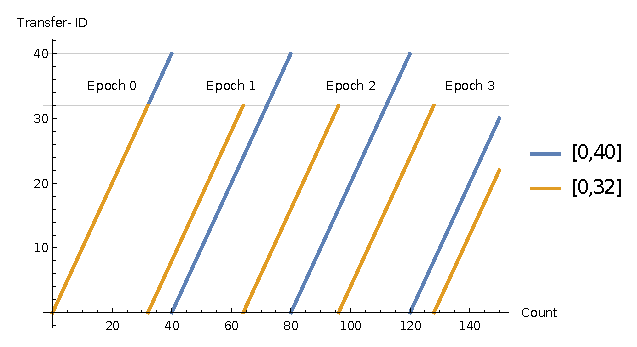
\includegraphics[width=0.6\textwidth]{transport/cyclic_transfer_id_redundant_transport}
        \caption{Issues with cyclic transfer-ID in heterogeneous redundant transports}
        \label{fig:transport_cyclic_transfer_id_redundant}
    \end{figure}
\end{remark}
\end{comment}

\subsection{Transfer transmission}

\subsubsection{Transmission timeout}

The transport frames of a time-sensitive transfer whose payload has lost relevance due to
its transmission being delayed should be removed from the transmission queue\footnote{%
    Trailing transport frames of partially transmitted multi-frame transfers should be removed as well.
    The objective of this recommendation is to ensure that obsolete data is not transmitted
    as it may have adverse effects on the system.
}.
The time interval between the point where the transfer is constructed and the point where it is considered
to have lost relevance is referred to as \emph{transmission timeout}.

% "Output port" sounds better but this term is not defined.
The transmission timeout should be documented for each outgoing transfer port.

\subsubsection{Pending service requests}

In the case of cyclic transfer-ID transports (section~\ref{sec:transport_transfer_id}),
implementations should ensure that upon a transfer-ID overflow a service client session
does not reuse the same transfer-ID value for more than one pending request simultaneously.

\subsubsection{Deterministic data loss mitigation}\label{sec:transport_deterministic_data_loss_mitigation}

Performance of transport networks where the probability of a successful transfer delivery
does not meet design requirements can be adjusted by repeating relevant outgoing transfers
under the same transfer-ID value\footnote{%
    Removal of intentionally duplicated transfers on the receiving side is natively guaranteed
    by this transport layer specification;
    no special activities are needed there to accommodate this feature.
}.
This tactic is referred to as \emph{deterministic data loss mitigation}\footnote{%
    Discussed in
    \url{https://forum.opencyphal.org/t/idempotent-interfaces-and-deterministic-data-loss-mitigation/643}.
}.

\subsubsection{Transmission over redundant transports}

Nodes equipped with redundant transports shall submit every outgoing transfer to the transmission queues of all
available redundant transports simultaneously\footnote{%
    The objective of this requirement is to guarantee that a redundant transport remains fully functional
    as long as at least one transport in the redundant group is functional.
}.
It is recognized that perfectly simultaneous transmission may not be possible due to different
utilization rates of the redundant transports, different phasing of their traffic, and/or application constraints,
in which case implementations should strive to minimize the temporal skew as long as that
does not increase the latency.

An exception to the above rule applies if the payload of the transfer is a function of
the identity of the transport instance that carries the transfer\footnote{%
    An example of such a special case is the time synchronization algorithm documented
    in section~\ref{sec:application_functions}.
}.

\subsection{Transfer reception}\label{sec:transport_transfer_reception}

\subsubsection{Definitions}

\emph{Transfer reassembly} is the real-time process of reconstruction of the transfer payload and its metadata from
a sequence of relevant transport frames.

\emph{Transfer-ID timeout} is a time interval whose semantics are explained below.
Implementations may define this value statically according to the application requirements.
Implementations may automatically adjust this value per session at runtime as a function of the
observed transfer reception interval.
Implementations should document the value of transfer-ID timeout or the rules of its computation.

\emph{Transport frame reception timestamp} specifies the moment of time when the frame is received by a node.
\emph{Transfer reception timestamp} is the reception timestamp of the earliest received frame of the transfer.

An \emph{ordered transfer sequence} is a sequence of transfers whose temporal order is
covariant with their transfer-ID values.

\subsubsection{Behaviors}

For a given session specifier, every unique transfer
(differentiated from other transfers in the same session by its transfer-ID)
shall be received at most once\footnote{%
    In other words, intentional and unintentional duplicates shall be removed.
    Intentional duplications are introduced by the deterministic data loss mitigation measure or redundant transports.
    Unintentional duplications may be introduced by various artifacts of the transport network.
}.

For a given session specifier, a successfully reassembled transfer that is
temporally separated from any other successfully reassembled transfer under the same session specifier
by more than the transfer-ID timeout is considered unique regardless of its transfer-ID value.

If the optimal transfer-ID timeout value for a given session cannot be known in advance,
it can be computed at runtime on a per-session basis\footnote{%
    E.g., as a multiple of the average transfer reception interval.
}.
The parameters of such computation are to be chosen according to the requirements of the application,
but they should always be documented.

The transfer-ID timeout used with service response transfers should be zero\footnote{%
    With a non-zero transfer-ID timeout, responses may be lost if the server responds to multiple requests
    from the same client not in the order of their arrival.
    There is no risk of response duplication because the client will retire the pending request entry
    once its first response is received, ignoring subsequent duplicates.
}.

\begin{remark}
    Low transfer-ID timeout values increase the risk of undetected transfer duplication when such transfers
    are significantly delayed due to network congestion,
    which is possible with very low-priority transfers when the network load is high.

    High transfer-ID timeout values increase the risk of an undetected transfer loss
    when a remote node suffers a loss of state (e.g., due to a software reset).

    The ability to auto-detect the optimal transfer-ID timeout value per session at runtime ensures that the
    application can find the optimal balance even if the temporal properties of the network are not known in advance.
    As a practical example, an implementation could compute the exponential moving average of the
    transfer reception interval $x$ for a given session and define the transfer-ID timeout as $2x$.

    It is important to note that the automatic adjustment of the transfer-ID timeout should only be done
    on a per-session basis rather than for the entire port, because there may be multiple remote nodes
    emitting transfers on the same port at different rates.
    For example, if one node emits transfers at a rate $r$ transfers per second, and another node emits transfers
    on the same port at a much higher rate $100r$, the resulting auto-detected transfer-ID timeout might be
    too low, creating the risk of accepting duplicates.
\end{remark}

Implementations are recommended, but not required, to support reassembly of
multi-frame transfers where the temporal ordering of the transport frames is distorted.

\begin{remark}
    For a certain category of transport implementations, reassembly of multi-frame transfers from an
    unordered transport frame sequence increases the probability of successful delivery if
    the probability of a transport frame loss is non-zero and transport frames are intentionally duplicated.

    Such intentional duplication occurs in redundant transports and if deterministic data loss mitigation is used.
    The reason is that the loss of a single transport frame is observed by the receiving node as its relocation
    from its original position in the sequence to the position of its duplicate.
\end{remark}

Reassembled transfers shall form an ordered transfer sequence.

For a cyclic transfer-ID redundant transport whose redundant group contains $n$ transports,
if up to $n-1$ transports in the redundant group lose the ability to exchange transport frames between nodes,
the transfer reassembly process shall be able to restore nominal functionality
in an amount of time that does not exceed the transfer-ID timeout.

\begin{remark}
    Cyclic transfer-ID transport implementations are recommended to insert a delay before performing
    an automatic fail-over.
    As indicated in the normative description, the delay may be arbitrary as long as it does not exceed the
    transfer-ID timeout value.

    The fail-over delay allows implementations to uphold the transfer uniqueness requirement when the phasing of
    traffic on different transports within the redundant group differs by more than the transfer-ID overflow period.
\end{remark}

For a monotonic transfer-ID redundant transport whose redundant group contains $n$ transports,
if up to $n-1$ transports in the redundant group lose the ability to exchange transport frames between nodes,
the performance of the transfer reassembly process shall not be affected.

\begin{remark}
    Monotonic transfer-ID transport implementations are recommended to always accept the first transfer
    to arrive regardless of which transport within the redundant group it was delivered over.

    This behavior ensures that the total latency of a redundant transport equals the latency of the best-performing
    transport within the redundant group (i.e., the total latency equals the latency of the fastest transport).
    Since a monotonic transfer-ID does not overflow, there is no risk of failing to uphold the uniqueness guarantee
    unlike with the case of cyclic transfer-ID.
\end{remark}

If anonymous transfers are supported by the concrete transport,
reassembly of anonymous transfers shall be implemented by unconditional acceptance of their transport frames.
Requirements pertaining to ordering and uniqueness do not apply.

\begin{remark}
    Regardless of the concrete transport in use and its capabilities,
    Cyphal provides the following guarantees (excluding anonymous transfers):

    \begin{itemize}
        \item Removal of duplicates. If a transfer is delivered, it is guaranteed that it is delivered once,
              even if intentionally duplicated by the origin.
        \item Correct ordering. Received transfers are ordered according to their transfer-ID values.
        \item Deterministic automatic fail-over in the event of a failure of a transport (or several)
              in a redundant group.
    \end{itemize}

    For anonymous transfers, ordering and uniqueness are impossible to enforce
    because anonymous transfers that originate from different nodes may share the same session specifier.

    Reassembly of transfers from redundant interfaces may be implemented either on the per-transport-frame level
    or on the per-transfer level.
    The former amounts to receiving individual transport frames from redundant interfaces
    which are then used for reassembly; it can be seen that this method requires that all transports in the
    redundant group use identical application-level MTU (i.e., same number of transfer payload bytes per frame).
    The latter can be implemented by treating each transport in the redundant group separately,
    so that each runs an independent transfer reassembly process, whose outputs are then deduplicated
    on the per-transfer level; this method may be more computationally complex but it provides greater flexibility.
    A detailed discussion is omitted because it is outside of the scope of this specification.
\end{remark}

\clearpage\section{Cyphal/CAN}\label{sec:transport_can}

\hyphenation{Cyphal/CAN}  % Disable hyphenation.

This section specifies a concrete transport based on ISO 11898 CAN bus.
Throughout this section, ``CAN'' implies both Classic CAN 2.0 and CAN FD, unless specifically noted otherwise.
CAN FD should be considered the primary transport protocol.

\begin{CyphalSimpleTable}{Cyphal/CAN transport capabilities}{|l X l|}
    \label{table:transport_can_capabilities}
    Parameter & Value & References \\

    Maximum node-ID value &
    127 (7 bits wide). &
    \ref{sec:basic} \\

    Transfer-ID mode &
    Cyclic, modulo 32. &
    \ref{sec:transport_transfer_id} \\

    Number of transfer priority levels &
    8 (no additional levels). &
    \ref{sec:transport_transfer_priority} \\

    Largest single-frame transfer payload &
    Classic CAN -- 7~bytes, CAN FD -- up to 63~bytes. &
    \ref{sec:transport_transfer_payload} \\

    Anonymous transfers &
    Supported with non-deterministic collision resolution policy. &
    \ref{sec:transport_route_specifier} \\
\end{CyphalSimpleTable}

\subsection{CAN ID field}

Cyphal/CAN transport frames are CAN 2.0B frames.
The 29-bit CAN ID encodes the session specifier\footnote{Section~\ref{sec:transport_session_specifier}.}
of the transfer it belongs to along with its priority.
The CAN data field of every frame contains the transfer payload
(or, in the case of multi-frame transfers, a fraction thereof), the transfer-ID, and other metadata.

Cyphal/CAN can share the same bus with other high-level CAN bus protocols provided that they
do not make use of CAN 2.0B frames\footnote{For example, CANOpen or CANaerospace.}.
However, future revisions of Cyphal/CAN may utilize CAN 2.0A as well,
so backward compatibility with other high-level CAN bus protocols is not guaranteed.

Cyphal/CAN utilizes two different CAN ID bit layouts for message transfers and service transfers.
The bit layouts are summarized on figure~\ref{fig:transport_can_id_structure}.
Tables~\ref{table:transport_can_id_fields_message_transfer} and~\ref{table:transport_can_id_fields_service_transfer}
summarize the purpose of each field and their permitted values
for message transfers and service transfers, respectively.

% Please do not remove the hard placement specifier [H], it is needed to keep elements ordered.
\begin{figure}[H]
    \centering
    \resizebox{\textwidth}{!}{
        \footnotesize
        \begin{tabular}{|l|c|c|c|c|c|c|c|c|c|c|c|c|c|c|c|c|c|c|c|c|c|c|c|c|c|c|c|c|c|} \hline
            %
            % Message transfer
            %
            \multirow{2}{*}{\textbf{Message}} &
            \multicolumn{4}{c|}{Service, not message} &
            \multicolumn{4}{c|}{Anonymous} &
            \multicolumn{13}{c|}{\multirow{2}{*}{Subject-ID}} &
            \multicolumn{1}{c|}{\multirow{2}{*}{R}} &
            \multicolumn{7}{c|}{\multirow{2}{*}{Source node-ID}}
            \\\cline{2-4} \cline{7-9}

            &
            \multicolumn{3}{c|}{Priority}
            &
            &
            &
            R &
            R &
            R &
            \multicolumn{13}{c|}{} &
            &
            \multicolumn{7}{c|}{}
            \\

            \textbf{Values} &
            \multicolumn{3}{c|}{$[0, 7]$} &
            $0$ &
            $\mathbb{B}$ &
            $0$ &
            $1$ &
            $1$ &
            \multicolumn{13}{c|}{$[0, 8191]$} &
            $0$ &
            \multicolumn{7}{c|}{$[0, 127]$}
            \\\hline

            \textbf{CAN ID bit} &
            28 & 27 & 26 & 25 & 24 & 23 & 22 & 21 & 20 & 19 & 18 & 17 & 16 & 15 &
            14 & 13 & 12 & 11 & 10 &  9 &  8 &  7 &  6 &  5 &  4 &  3 &  2 &  1 &  0
            \\\hline

            \textbf{CAN ID byte} &
            \multicolumn{5}{c|}{3} & \multicolumn{8}{c|}{2} & \multicolumn{8}{c|}{1} & \multicolumn{8}{c|}{0}
            \\\hline

            \multicolumn{30}{c}{} \\ \hline % Table separator

            %
            % Service transfer
            %
            \multirow{2}{*}{\textbf{Service}} &
            \multicolumn{4}{c|}{Service, not message} &
            \multicolumn{5}{c|}{Request, not response} &
            \multicolumn{6}{c|}{} &
            \multicolumn{7}{c|}{\multirow{2}{*}{Destination node-ID}} &
            \multicolumn{7}{c|}{\multirow{2}{*}{Source node-ID}}
            \\\cline{2-4} \cline{7-10}

            &
            \multicolumn{3}{c|}{Priority} &
            &
            &
            R &
            \multicolumn{9}{c|}{Service-ID} &
            \multicolumn{7}{c|}{} &
            \multicolumn{7}{c|}{}
            \\

            \textbf{Values} &
            \multicolumn{3}{c|}{$[0, 7]$} &
            $1$ &
            $\mathbb{B}$ &
            $0$ &
            \multicolumn{9}{c|}{$[0, 511]$} &
            \multicolumn{7}{c|}{$[0, 127]$} &
            \multicolumn{7}{c|}{$[0, 127]$}
            \\\hline

            \textbf{CAN ID bit} &
            28 & 27 & 26 & 25 & 24 & 23 & 22 & 21 & 20 & 19 & 18 & 17 & 16 & 15 &
            14 & 13 & 12 & 11 & 10 &  9 &  8 &  7 &  6 &  5 &  4 &  3 &  2 &  1 &  0
            \\\hline

            \textbf{CAN ID byte} &
            \multicolumn{5}{c|}{3} & \multicolumn{8}{c|}{2} & \multicolumn{8}{c|}{1} & \multicolumn{8}{c|}{0}
            \\\hline
        \end{tabular}
    }
    \caption{CAN ID bit layout}\label{fig:transport_can_id_structure}
\end{figure}

\begin{CyphalSimpleTable}[wide]{CAN ID bit fields for message transfers}{|l l l X|}
    \label{table:transport_can_id_fields_message_transfer}
    Field               & Width & Valid values  & Description \\

    Transfer priority   & 3     & $[0, 7]$ (any)    & Section~\ref{sec:transport_transfer_priority}. \\

    Service, not message & 1    & $0$               & Always zero for message transfers. \\

    Anonymous           & 1     & $\{0, 1\}$ (any)  & Zero for regular message transfers,
                                                      one for anonymous transfers. \\

    Reserved bit 23     & 1     & $0$               & Discard frame if this field has a different value. \\

    % The asymmetric requirement to transmit only 1 and accept any value is due to the need to ensure compatibility
    % with the implementations following the v1-alpha spec, where the width of the subject-ID field was 15 bit
    % (two bits wider). We keep the most significant bits set to ensure the compatibility of the regulated subject-IDs
    % between v1-alpha and v1-beta. Ensuring the compatibility of unregulated subject-IDs is far less important because
    % generally, they are easily changeable.
    %
    % Such backward-compatible change renders these two bits unusable for the possible future expansion of the
    % subject-ID field, but this is fine, because shall the expansion become imminent, we can always flip R7 from 0
    % to 1, and thus pave the way for a completely new bit layout format with a wider subject-ID. Meanwhile, R21 and
    % R22 can be leveraged for some additional optional features.
    Reserved bit 22     & 1     & $1$, any          & Transmit $1$; ignore (do not check) when receiving. \\
    Reserved bit 21     & 1     & $1$, any          & Transmit $1$; ignore (do not check) when receiving. \\

    Subject-ID          & 13    & $[0, 8191]$ (any) & Subject-ID of the current message transfer. \\

    Reserved bit 7      & 1     & $0$               & Discard frame if this field has a different value. \\

    Source node-ID      & 7     & $[0, 127]$ (any)  & Node-ID of the origin.
                                                      For anonymous transfers, this field contains a pseudo-ID instead,
                                                      as described in
                                                      section~\ref{sec:transport_can_source_node_pseudo_id}. \\
\end{CyphalSimpleTable}

\begin{CyphalSimpleTable}[wide]{CAN ID bit fields for service transfers}{|l l l X|}
    \label{table:transport_can_id_fields_service_transfer}
    Field               & Width & Valid values  & Description \\

    Transfer priority   & 3     & $[0, 7]$ (any)    & Section~\ref{sec:transport_transfer_priority}. \\

    Service, not message & 1    & $1$               & Always one for service transfers. \\

    Request, not response & 1   & $\{0, 1\}$ (any)  & One for service request, zero for service response. \\

    Reserved bit 23     & 1     & $0$               & Discard frame if this field has a different value. \\

    Service-ID          & 9     & $[0, 511]$ (any)  & Service-ID of the encoded service object
                                                      (request or response). \\

    Destination node-ID & 7     & $[0, 127]$ (any)  & Node-ID of the destination:
                                                      server if request, client if response. \\

    Source node-ID      & 7     & $[0, 127]$ (any)  & Node-ID of the origin:
                                                      client if request, server if response. \\
\end{CyphalSimpleTable}

\subsubsection{Transfer priority}

Valid values for transfer priority range from 0 to 7, inclusively,
where 0 corresponds to the highest priority, and 7 corresponds to the lowest priority
(according to the CAN bus arbitration policy).

In multi-frame transfers, the value of the priority field shall be identical for all frames of the transfer.

\begin{remark}[breakable]
    When multiple transfers of different types with the same priority contest for bus access,
    the following precedence is ensured (from higher priority to lower priority):

    \begin{enumerate}
        \item Message transfers (the primary method of data exchange in Cyphal networks).
        \item Anonymous (message) transfers.
        \item Service response transfers (preempt requests).
        \item Service request transfers (responses take precedence over requests to make service calls more atomic
              and reduce the number of pending states in the system).
    \end{enumerate}

    Mnemonics for transfer priority levels are provided in section~\ref{sec:transport_transfer_priority},
    and their mapping to the Cyphal/CAN priority field is as follows:

    \begin{CyphalCompactTable}{|l X|}
        Priority field value    & Mnemonic name \\
        0                       & Exceptional   \\
        1                       & Immediate     \\
        2                       & Fast          \\
        3                       & High          \\
        4                       & Nominal       \\
        5                       & Low           \\
        6                       & Slow          \\
        7                       & Optional      \\
    \end{CyphalCompactTable}

    Since the value of transfer priority is required to be the same for all frames in a transfer,
    it follows that the value of the CAN ID is guaranteed to be the same for all CAN frames of the transfer.
    Given a constant transfer priority value, all CAN frames under a given session specifier will be equal.
\end{remark}

\subsubsection{Source node-ID field in anonymous transfers}\label{sec:transport_can_source_node_pseudo_id}

The source node-ID field of anonymous transfers shall be initialized with a pseudorandom \emph{pseudo-ID} value.
The source of the pseudorandom data used for the pseudo-ID shall aim to produce different values
for different CAN frame data field values.

A node transmitting an anonymous transfer shall abort its transmission and discard it upon detection of a bus error.
Some method of media access control should be used at the application level for further conflict resolution.

\begin{remark}[breakable]
    CAN bus does not allow different nodes to transmit CAN frames with different data under the same CAN ID value.
    Owing to the fact that the CAN ID includes the node-ID of the transmitting node,
    this restriction does not affect non-anonymous transfers.
    However, anonymous transfers would violate this restriction because their source node-ID is not defined,
    hence the additional measures described in this section.

    A possible way of initializing the source node pseudo-ID value is to compute the arithmetic sum
    of all bytes of the transfer payload, taking the least significant bits of the result as the pseudo-ID
    (usage of stronger hashes is encouraged).
    Implementations that adopt this approach will be using the same pseudo-ID value for identical transfer payloads,
    which is acceptable since this will not trigger an error on the bus.

    Because the set of possible pseudo-ID values is small,
    a collision where multiple nodes emit CAN frames with different data but the same CAN ID is likely to happen
    despite the randomization measures described here.
    Therefore, if anonymous transfers are used,
    implementations shall account for possible errors on the CAN bus triggered by CAN ID collisions.

    Automatic retransmission should be disabled for anonymous transfers (like in TTCAN).
    This measure allows the protocol to prevent temporary disruptions that may occur if the automatic
    retransmission on bus error is not suppressed.

    Additional bus access control logic is needed at the application level because
    the possibility of identifier collisions in anonymous frames undermines the access control logic implemented
    in CAN bus controller hardware.

    The described principles make anonymous transfers highly non-deterministic and inefficient.
    This is considered acceptable because the scope of anonymous transfers is limited to a very narrow set of use
    cases which tolerate their downsides. The Cyphal specification employs anonymous transfers only for the
    plug-and-play feature defined in section~\ref{sec:application_functions}.
    Deterministic applications are advised to avoid reliance on anonymous transfers completely.

    None of the above considerations affect nodes that do not transmit anonymous transfers.
\end{remark}

\subsection{CAN data field}

\subsubsection{Layout}

Cyphal/CAN utilizes a fixed layout of the CAN data field:
the last byte of the CAN data field contains the metadata, it is referred to as the \emph{tail byte}.
The preceding bytes of the data field contain the transfer payload,
which may be extended with padding bytes and transfer CRC.

A CAN frame whose data field contains less than one byte is not a valid Cyphal/CAN frame.

The bit layout of the tail byte is shown in table~\ref{table:transport_can_tail_byte}.

% Please do not remove the hard placement specifier [H], it is needed to keep tables ordered.
\begin{table}[H]\caption{Tail byte structure}\label{table:transport_can_tail_byte}
    \begin{tabu}{| c l | X[c2] X[c3] |}
        \hline
        \rowfont{\bfseries}
        Bit & Field & Single-frame transfers & Multi-frame transfers \\
        \hline
        7   & \textbf{Start of transfer}& Always 1  & First frame: 1, otherwise 0. \\\hline
        6   & \textbf{End of transfer}  & Always 1  & Last frame: 1, otherwise 0. \\\hline
        5   & \textbf{Toggle bit}       & Always 1  & First frame: 1, then alternates;
                                                      section~\ref{sec:transport_can_toggle_bit}. \\\hline
        4   &                           & \multicolumn{2}{c|}{} \\
        3   &                           & \multicolumn{2}{c|}{Modulo 32 (range [0, 31])} \\
        2   & \textbf{Transfer-ID}      & \multicolumn{2}{c|}{section~\ref{sec:transport_transfer_id}} \\
        1   &                           & \multicolumn{2}{c|}{} \\
        0   &                           & \multicolumn{2}{c|}{\footnotesize{(least significant bit)}} \\
        \hline
    \end{tabu}
\end{table}

\subsubsection{Toggle bit}\label{sec:transport_can_toggle_bit}

Transport frames that form a multi-frame transfer are equipped with a \emph{toggle bit}
which alternates its state every frame within the transfer for frame deduplication purposes\footnote{%
    A frame that appears valid to the receiving node may under certain conditions appear invalid to the transmitter,
    triggering the latter to retransmit the frame, in which case it will be duplicated on the side of the receiver.
}.

\subsubsection{Transfer payload decomposition}

The transport-layer MTU of Classic CAN-based implementations shall be 8 bytes (the maximum).
The transport-layer MTU of CAN FD-based implementations should be 64 bytes (the maximum).

CAN FD does not guarantee byte-level granularity of the CAN data field length.
If the desired length of the CAN data field cannot be represented due to the granularity constraints,
zero padding bytes are used.

In single-frame transfers, padding bytes are inserted between the end of the payload and the tail byte.

In multi-frame transfers, the transfer payload is appended with trailing zero padding bytes
followed by the transfer CRC (section~\ref{sec:transport_can_transfer_crc}).
All transport frames of a multi-frame transfer except the last one shall fully utilize the available
data field capacity; hence, padding is unnecessary there.
The number of padding bytes is computed so that the length granularity constraints
for the last frame of the transfer are satisfied.

\begin{remark}
    Usage of padding bytes implies that when a serialized message is being deserialized by a receiving node,
    the byte sequence used for deserialization may be longer than the actual byte sequence generated by the
    emitting node during serialization.
    This behavior is compatible with the DSDL specification.

    The weak MTU requirement for CAN FD is designed to avoid compatibility issues.
\end{remark}

\subsubsection{Transfer CRC}\label{sec:transport_can_transfer_crc}

Payload of multi-frame transfers is extended with a transfer CRC for validating the correctness of their reassembly.
Transfer CRC is not used with single-frame transfers.

The transfer CRC is computed over the entire payload of the multi-frame transfer
plus the trailing padding bytes, if any.
The resulting CRC value is appended to the transfer payload after the padding bytes (if any)
in the \emph{big-endian byte order} (most significant byte first)\footnote{%
    This is the native byte order for this CRC function.
}.

The CRC function is the standard CRC-16-CCITT:
initial value $\mathrm{FFFF}_{16}$, polynomial $\mathrm{1021}_{16}$,
not reversed, no output XOR, big endian.
The value for an input sequence $\left(49, 50, \ldots, 56, 57\right)$ is $\mathrm{29B1}_{16}$.
The following code snippet provides a basic implementation of the transfer CRC algorithm in C++
(LUT-based alternatives exist).

\begin{samepage}
\begin{minted}{cpp}
#include <cstdint>
#include <cstddef>

/// Cyphal/CAN transfer CRC function implementation. License: CC0, no copyright reserved.
class CANTransferCRC
{
    std::uint16_t value_ = 0xFFFFU;

public:
    void add(const std::uint8_t byte)
    {
        value_ ^= static_cast<std::uint16_t>(byte) << 8U;
        for (std::uint8_t bit = 8; bit > 0; --bit)
        {
            if ((value_ & 0x8000U) != 0)
            {
                value_ = (value_ << 1U) ^ 0x1021U;
            }
            else
            {
                value_ = value_ << 1U;
            }
        }
    }

    void add(const std::uint8_t* bytes, std::size_t length)
    {
        while (length-- > 0)
        {
            add(*bytes++);
        }
    }

    [[nodiscard]] std::uint16_t get() const { return value_; }
};
\end{minted}
\end{samepage}

\subsection{Examples}

\begin{remark}[breakable]
    Heartbeat from node-ID 42, nominal priority level,
    uptime starting from 0 and then incrementing by one every transfer, health status is 0,
    operating mode is 1, vendor-specific status code 161 ($A1_{16}$):

    \begin{CyphalCompactTable}{|l l|}
        CAN ID (hex)      & CAN data (hex)          \\
        \texttt{107D552A} & \texttt{00 00 00 00 00 01 A1 E0} \\
        \texttt{107D552A} & \texttt{01 00 00 00 00 01 A1 E1} \\
        \texttt{107D552A} & \texttt{02 00 00 00 00 01 A1 E2} \\
        \texttt{107D552A} & \texttt{03 00 00 00 00 01 A1 E3} \\
    \end{CyphalCompactTable}

    \verb|uavcan.primitive.String.1.0| under subject-ID 4919 ($1337_{16}$) published by an anonymous node,
    the string is ``\verb|Hello world!|'' (ASCII); one byte of zero padding can be seen between
    the payload and the tail byte:

    \begin{CyphalCompactTable}{|l l|}
        CAN ID (hex)      & CAN data (hex)                                           \\
        \texttt{11133775} & \texttt{0C 00 48 65 6C 6C 6F 20 77 6F 72 6C 64 21 00 E0} \\
        \texttt{11133775} & \texttt{0C 00 48 65 6C 6C 6F 20 77 6F 72 6C 64 21 00 E1} \\
        \texttt{11133775} & \texttt{0C 00 48 65 6C 6C 6F 20 77 6F 72 6C 64 21 00 E2} \\
        \texttt{11133775} & \texttt{0C 00 48 65 6C 6C 6F 20 77 6F 72 6C 64 21 00 E3} \\
    \end{CyphalCompactTable}

    Node info request from node 123 to node 42 via Classic CAN, then response;
    notice how the transfer CRC is scattered across two frames:

    \begin{CyphalCompactTable}{|l l l X|}
        CAN ID (hex)      & CAN data (hex)                                  & ASCII             & Comment \\

        \texttt{136B957B} & \texttt{E1}                                     & \texttt{.}        &
        The request contains no payload. \\

        \texttt{126BBDAA} & \texttt{01 00 00 00 01 00 00 A1}                & \texttt{........} &
        Start of response, toggle bit is set. \\

        \texttt{126BBDAA} & \texttt{00 00 00 00 00 00 00 01}                & \texttt{........} &
        Toggle bit is cleared. \\

        \texttt{126BBDAA} & \texttt{00 00 00 00 00 00 00 21}                & \texttt{.......!} &
        Toggle bit is set. \\

        \texttt{126BBDAA} & \texttt{00 00 00 00 00 00 00 01}                & \texttt{........} &
        Etc. \\

        \texttt{126BBDAA} & \texttt{00 00 \underline{24} 6F 72 67 2E 21}    & \texttt{..\underline{\$}org.!} &
        Array (string) length prefix. \\

        \texttt{126BBDAA} & \texttt{75 61 76 63 61 6E 2E 01}                & \texttt{uavcan..} &
        \\

        \texttt{126BBDAA} & \texttt{70 79 75 61 76 63 61 21}                & \texttt{pyuavca!} &
        \\

        \texttt{126BBDAA} & \texttt{6E 2E 64 65 6D 6F 2E 01}                & \texttt{n.demo..} &
        \\

        \texttt{126BBDAA} & \texttt{62 61 73 69 63 5F 75 21}                & \texttt{basic\_u!} &
        \\

        \texttt{126BBDAA} & \texttt{73 61 67 65 00 00 \underline{9A} 01}    & \texttt{sage..\underline{.}.} &
        Transfer CRC, MSB. \\

        \texttt{126BBDAA} & \texttt{\underline{E7} 61}                      & \texttt{\underline{.}a}       &
        Transfer CRC, LSB. \\
    \end{CyphalCompactTable}

    \verb|uavcan.primitive.array.Natural8.1.0| under subject-ID 4919 ($1337_{16}$) published by node 59,
    the array contains an arithmetic sequence $\left(0, 1, 2, \ldots{}, 89, 90, 91\right)$;
    the transport MTU is 64 bytes:

    \begin{CyphalCompactTable}{|l X[2] X|}
        CAN ID (hex)      & CAN data (hex) & Comment \\
        \texttt{1013373B} &
        \texttt{%
            5C 00 00 01 02 03 04 05 06 07 08 09 0A 0B 0C 0D 0E 0F 10 11 12 13 14 15 16 17 18 19 1A 1B 1C 1D 1E 1F 20
            21 22 23 24 25 26 27 28 29 2A 2B 2C 2D 2E 2F 30 31 32 33 34 35 36 37 38 39 3A 3B 3C A0
        } &
        First frame: 1.~payload (array length prefix is 92); 2.~tail byte. \\

        \texttt{1013373B} &
        \texttt{%
            3D 3E 3F 40 41 42 43 44 45 46 47 48 49 4A 4B 4C 4D 4E 4F 50 51 52 53 54 55 56 57 58 59 5A 5B
            \underline{00} \underline{00} \underline{00} \underline{00} \underline{00} \underline{00} \underline{00}
            \underline{00} \underline{00} \underline{00} \underline{00} \underline{00} \underline{00} \underline{00}
            \textbf{BC} \textbf{19} 40
        } &
        Last frame: 1.~payload; 2.~padding (underlined); 3.~transfer CRC (bold); 4.~tail byte. \\
    \end{CyphalCompactTable}
\end{remark}

\subsection{Software design considerations}

\subsubsection{Ordered transmission}

The CAN controller driver software shall guarantee that CAN frames with identical CAN ID values
will be transmitted in their order of appearance in the transmission queue\footnote{%
    This is because multi-frame transfers use identical CAN ID for all frames of the transfer,
    and Cyphal requires that all frames of a multi-frame transfer shall be transmitted in the correct order.
}.

\subsubsection{Transmission timestamping}

\begin{remark}[breakable]
    Certain application-level functions of Cyphal may require the driver to timestamp outgoing transport frames,
    e.g., the time synchronization function.
    A sensible approach to transmission timestamping is built around the concept of \emph{loop-back frames},
    which is described here.

    If the application needs to timestamp an outgoing frame, it sets a special flag -- the \emph{loop-back flag} --
    on the frame before sending it to the driver.
    The driver would then automatically re-enqueue this frame back into the reception queue once it is transmitted
    (keeping the loop-back flag set so that the application is able to distinguish the loop-back
    frame from regular received traffic).
    The timestamp of the loop-backed frame would be of the moment when it was delivered to the bus.

    The advantage of the loop-back based approach is that it relies on the same interface between
    the application and the driver that is used for regular communications.
    No complex and dangerous callbacks or write-backs from interrupt handlers are involved.
\end{remark}

\subsubsection{Inner priority inversion}

Implementations should take necessary precautions against the problem of inner priority inversion.

\begin{remark}[breakable]
    Suppose the application needs to emit a frame with the CAN ID $X$.
    The frame is submitted to the CAN controller's registers and the transmission is started.
    Suppose that afterwards it turned out that there is a new frame with the CAN ID $(X-1)$ that needs to be sent,
    too, but the previous frame $X$ is in the way, and it is blocking the transmission of the new frame.
    This may turn into a problem if the lower-priority frame is losing arbitration on the bus due
    to the traffic on the bus having higher priority than the current frame,
    but lower priority than the next frame that is waiting in the queue.

    A naive solution to this is to continuously check whether the priority of the frame that is currently being
    transmitted by the CAN controller is lower than the priority of the next frame in the queue, and if it is,
    abort transmission of the current frame, move it back to the transmission queue,
    and begin transmission of the new one instead.
    This approach, however, has a hidden race condition:
    the old frame may be aborted at the moment when it has already been received by remote nodes,
    which means that the next time it is re-transmitted, the remote nodes will see it duplicated.
    Additionally, this approach increases the complexity of the driver and can possibly affect
    its throughput and latency.

    Most CAN controllers offer a robust solution to the problem:
    they have multiple transmission mailboxes (usually at least 3),
    and the controller always chooses for transmission the mailbox which contains the highest priority frame.
    This provides the application with a possibility to avoid the inner priority inversion problem:
    whenever a new transmission is initiated, the application should check whether the priority of the next frame
    is higher than any of the other frames that are already awaiting transmission.
    If there is at least one higher-priority frame pending,
    the application doesn't move the new one to the controller's transmission mailboxes,
    it remains in the queue.
    Otherwise, if the new frame has a higher priority level than all of the pending frames,
    it is pushed to the controller's transmission mailboxes and removed from the queue.
    In the latter case, if a lower-priority frame loses arbitration,
    the controller would postpone its transmission and try transmitting the higher-priority one instead.
    That resolves the problem.

    There is an interesting extreme case, however.
    Imagine a controller equipped with $N$ transmission mailboxes.
    Suppose the application needs to emit $N$ frames in the increasing order of priority,
    which leads to all of the transmission mailboxes of the controller being occupied.
    Now, if all of the conditions below are satisfied, the system ends up with a priority inversion condition
    nevertheless, despite the measures described above:

    \begin{itemize}
        \item The highest-priority pending CAN frame cannot be transmitted due to the bus being saturated
        with a higher-priority traffic.
        \item The application needs to emit a new frame which has a higher priority than that which saturates the bus.
    \end{itemize}

    If both hold, a priority inversion is afoot because there is no free transmission mailbox to
    inject the new higher-priority frame into.
    The scenario is extremely unlikely, however;
    it is also possible to construct the application in a way that would preclude the problem,
    e.g., by limiting the number of simultaneously used distinct CAN ID values.

    The following pseudocode demonstrates the principles explained above:

    \begin{samepage}
    \begin{minted}{cpp}
    // Returns the index of the TX mailbox that can be used for the transmission of the newFrame
    // If none are available, returns -1.
    getFreeMailboxIndex(newFrame)
    {
        chosen_mailbox = -1     // By default, assume that no mailboxes are available

        for i = 0...NumberOfTxMailboxes
        {
            if isTxMailboxFree(i)
            {
                chosen_mailbox = i
                // Note: cannot break here, shall check all other mailboxes as well.
            }
            else
            {
                if not isFramePriorityHigher(newFrame, getFrameFromTxMailbox(i))
                {
                    chosen_mailbox = -1
                    break   // Denied - shall wait until this mailbox has finished transmitting
                }
            }
        }

        return chosen_mailbox
    }
    \end{minted}
    \end{samepage}
\end{remark}

\subsubsection{Automatic hardware acceptance filter configuration}

\begin{remark}[breakable]
    Most CAN controllers are equipped with hardware acceptance filters.
    Hardware acceptance filters reduce the application workload by ignoring irrelevant CAN frames on the bus
    by comparing their ID values against the set of relevant ID values configured by the application.

    There exist two common approaches to CAN hardware filtering:
    list-based and mask-based.
    In the case of the list-based approach, every CAN frame detected on the bus is compared
    against the set of reference CAN ID values provided by the application;
    only those frames that are found in the reference set are accepted.
    Due to the complex structure of the CAN ID field used by Cyphal,
    usage of the list-based filtering method with this protocol is impractical.

    Most CAN controller vendors implement mask-based filters,
    where the behavior of each filter is defined by two parameters: the mask $M$ and the reference ID $R$.
    Then, such filter accepts only those CAN frames for which the following bitwise logical condition holds
    true\footnote{Notation: $\land$ -- bitwise logical AND, $\oplus$ -- bitwise logical XOR,
    $\neg$ -- bitwise logical NOT.}:
    $$((X \land M) \oplus R) \leftrightarrow 0$$
    where $X$ is the CAN ID value of the evaluated frame.

    Complex Cyphal applications are often required to operate with more distinct transfers than there are
    acceptance filters available in the hardware.
    That creates the challenge of finding the optimal configuration of the available filters that meets the
    following criteria:
    \begin{itemize}
        \item All CAN frames needed by the application are accepted.
        \item The number of irrelevant frames (i.e., not used by the application) accepted from the bus is minimized.
    \end{itemize}

    The optimal configuration is a function of the number of available hardware filters,
    the set of distinct transfers needed by the application,
    and the expected frequency of occurrence of all possible distinct transfers on the bus.
    The latter is important because if there are to be irrelevant transfers,
    it makes sense to optimize the configuration so that the acceptance of less common irrelevant transfers
    is preferred over the more common irrelevant transfers, as that reduces the processing load on the application.

    The optimal configuration depends on the properties of the network the node is connected to.
    In the absence of the information about the network,
    or if the properties of the network are expected to change frequently,
    it is possible to resort to a quasi-optimal configuration which assumes that
    the occurrence of all possible irrelevant transfers is equally probable.
    As such, the quasi-optimal configuration is a function of only the number of available hardware filters
    and the set of distinct transfers needed by the application.

    The quasi-optimal configuration can be easily found automatically.
    Certain implementations of the Cyphal protocol stack include this functionality,
    allowing the application to easily adjust the configuration of the hardware acceptance filters
    using a very simple API.

    A quasi-optimal hardware acceptance filter configuration algorithm is described below.
    The approach was first proposed by P. Kirienko and I. Sheremet in 2015.

    First, the bitwise \emph{filter merge} operation is defined on filter configurations $A$ and $B$.
    The set of CAN frames accepted by the merged filter configuration is a superset of
    those accepted by $A$ and $B$.
    The definition is as follows:
    \begin{equation*}
    \begin{split}
        m_M(R_A, R_B, M_A, M_B) & = M_A \land M_B \land \neg (R_A \oplus R_B) \\
        m_R(R_A, R_B, M_A, M_B) & = R_A \land m_M(R_A, R_B, M_A, M_B)
    \end{split}
    \end{equation*}

    The \emph{filter rank} is a function of the mask of the filter.
    The rank of a filter is a unitless quantity that defines in relative terms how selective the filter
    configuration is.
    The rank of a filter is proportional to the likelihood that the filter will reject a random CAN ID.
    In the context of hardware filtering, this quantity is conveniently representable via the number of bits set in
    the filter mask parameter (also known as \emph{population count}):
    \begin{equation*}
    r(M) =
    \begin{cases}
        0                                   &\mid M < 1 \\
        r(\lfloor\frac{M}{2}\rfloor)        &\mid M \bmod 2 = 0 \\
        r(\lfloor\frac{M}{2}\rfloor) + 1    &\mid M \bmod 2 \neq 0 \\
    \end{cases}
    \end{equation*}

    Having the low-level operations defined, we can proceed to define the whole algorithm.
    First, construct the initial set of CAN acceptance filter configurations
    according to the requirements of the application.
    Then, as long as the number of configurations in the set exceeds the number of available
    hardware acceptance filters, repeat the following:
    \begin{enumerate}
        \item Find the pair $A$, $B$ of configurations in the set for which $r(m_M(R_A, R_B, M_A, M_B))$ is maximized.
        \item Remove $A$ and $B$ from the set of configurations.
        \item Add a new configuration $X$ to the set of configurations, where
        $M_X = m_M(R_A, R_B, M_A, M_B)$, and $R_X = m_R(R_A, R_B, M_A, M_B)$.
    \end{enumerate}

    The algorithm reduces the number of filter configurations by one at each iteration,
    until the number of available hardware filters is sufficient to accommodate the whole set of configurations.
\end{remark}

\clearpage\section{Cyphal/UDP}\label{sec:transport_can}

\hyphenation{Cyphal/UDP}  % Disable hyphenation.

\subsection{Overview}

This section specifies a concrete transport based on the UDP/IPv4 protocol\footnote{%
    Support for IPv6 may appear in future versions of this specification.
}, as specified in IETF RFC~768.
\textbf{
    As of this version, the Cyphal/UDP specification remains experimental.
    Breaking changes affecting wire compatibility are possible.
}

Cyphal/UDP is intended for low-latency, high-throughput intravehicular Ethernet networks with complex topologies,
which may be switched, multi-drop, or mixed.
A network utilizing Cyphal/UDP can be built with standards-compliant commercial off-the-shelf
networking equipment and software.

Cyphal/UDP relies exclusively on IP multicast traffic defined in IETF RFC~1112 for all communication\footnote{%
    For rationale, refer to \url{https://forum.opencyphal.org/t/1765}.
}.
The entirety of the session specifier (section~\ref{sec:transport_session_specifier})
is reified through the multicast group address.
The transfer-ID, transfer priority, and the multi-frame transfer reassembly metadata are allocated in the
Cyphal-specific fixed-size UDP datagram header.
In this transport, a UDP datagram represents a single Cyphal transport frame.
All UDP datagrams are addressed to the same, fixed, destination port,
while the source port and the source address bear no relevance for the protocol and thus can be arbitrary.

\begin{CyphalSimpleTable}{Cyphal/UDP transport capabilities\label{table:transport_can_capabilities}}{|l X l|}
    Parameter & Value & References \\

    Maximum node-ID value &
    65534 (16 bits wide). &
    \ref{sec:basic} \\

    Transfer-ID mode &
    Monotonic, 64 bits wide. &
    \ref{sec:transport_transfer_id} \\

    Number of transfer priority levels &
    8 (no additional levels). &
    \ref{sec:transport_transfer_priority} \\

    Largest single-frame transfer payload &
    % 480 bytes = 508 bytes minus 24 bytes for the Cyphal/UDP header minus 4 bytes for the transfer CRC.
    % 65479 bytes = 65507 bytes minus 24 bytes for the Cyphal/UDP header minus 4 bytes for the transfer CRC.
    Implementation-defined, but not less than 480~bytes and not greater than 65479~bytes. &
    \ref{sec:transport_transfer_payload} \\

    Anonymous transfers &
    Available. &
    \ref{sec:transport_route_specifier} \\
\end{CyphalSimpleTable}

\subsection{UDP/IP endpoints and routing}

Transmission of a Cyphal/UDP transport frame is performed by sending a suitably constructed UDP datagram
to the destination IP multicast group address computed from the session specifier
(section~\ref{sec:transport_session_specifier})
as shown in figure~\ref{fig:transport_udp_multicast_group_address}
with the fixed destination port number \textbf{9382}.

\begin{figure}[H]
    \centering
    $$
    \overbrace{
        \underbrace{
            \texttt{\huge{1110}}
        }_{\substack{\text{RFC~1112} \\ \text{multicast} \\ \text{prefix}}}%
        \underbrace{
            \texttt{\huge{1111}}
        }_{\substack{\text{RFC~2365} \\ \text{administrative} \\ \text{scope}}}%
    }^{\text{Most significant octet}}%
    \texttt{\huge{.}}% ----------------------------------------
    \overbrace{
        \underbrace{
            \texttt{\huge{0}}
        }_{\substack{\text{RFC~2365} \\ \text{reserved} \\ \text{range}}}%
        \underbrace{
            \texttt{\huge{0}}
        }_{\substack{\text{address} \\ \text{version}}}%
        \underbrace{
            \texttt{\huge{00000}}
        }_{\substack{\text{reserved} \\ \text{keep zero}}}%
        \underbrace{
            \texttt{\huge{Z}}
        }_{\substack{\text{service,} \\ \text{not} \\ \text{message}}}%
    }^{\text{3rd octet}}%
    \texttt{\huge{.}}% ----------------------------------------
    \underbrace{
        \overbrace{\texttt{\huge{XXXXXXXX}}}^{\text{2nd octet}}
        \texttt{\huge{.}}
        \overbrace{\texttt{\huge{XXXXXXXX}}}^{\text{Least significant octet}}
    }_{\substack{\text{\textbf{if Z:} destination node-ID} \\ \text{\textbf{else:} subject-ID}}}%
    $$
    Numbers given in base-2.
    \caption{IP multicast group address structure\label{fig:transport_udp_multicast_group_address}}
\end{figure}

\begin{CyphalSimpleTable}[wide]{
    IP multicast group address bit fields\label{table:transport_udp_multicast_group_address}
}{|l l l l X|}
    Field & Offset & Width & Value & Description \\

    RFC~1112 multicast prefix &
    28 & 4 & $1110_2$ &
    \\

    RFC~2365 scope &
    24 & 4 & $1111_2$ &
    Selects the administratively scoped range 239.0.0.0/8 per RFC~2365
    to avoid collisions with well-known multicast groups. \\

    RFC~2365 reserved range &
    23 & 1 & $0_2$ &
    Selects the ad-hoc defined range 239.0.0.0/9 per RFC~2365. \\

    Cyphal/UDP address version &
    22 & 1 & $0_2$ &
    Deconflicts this layout with future revisions. \\

    Reserved &
    17 & 5 & $00000_2$ &
    May be used for domain-ID segregation in future versions. \\

    Z: service, not message &
    16 & 1 & any &
    Set for service transfers, cleared for message transfers. \\

    X if Z: destination node-ID &
    0 & 16 & $[0, 65534]$ &
    The destination node-ID of the current service transfer. \\

    X if not Z: subject-ID &
    0 & 16 & $[0, 8191]$ &
    The subject-ID of the current message transfer. \\
\end{CyphalSimpleTable}

A subscriber to certain Cyphal subjects will join the IP multicast groups corresponding to said subjects.
Likewise, a node that provides at least one RPC-service will join the IP multicast group corresponding to
its own node-ID\footnote{Observe that multicast groups are not differentiated by service-ID.}.

The IP address of a node bears no relevance for the protocol ---
multiple nodes may share the same IP address; likewise, a node may have more than one IP address.
Nodes on a Cyphal/UDP network are identified exclusively by their node-ID value\footnote{%
    A node that is registered on an IP network (e.g., via DHCP)
    still needs to obtain a node-ID value to participate in a Cyphal/UDP network.
    This may be done either through manual assignment or by using the plug-and-play node-ID allocation service
    (section~\ref{sec:application_functions_pnp}).
}.
The set of valid node-ID values for Cyphal/UDP is $[0, 65534]$.
Value 65535 is reserved to represent both the broadcast and anonymous node-ID, depending on context.

Sources of Cyphal/UDP traffic should set the packet TTL to 16 or higher\footnote{%
    RFC~1112 prescribes a default TTL of 1,
    but this is not sufficient for most applications Cyphal/UDP is intended for.
}.

The DSCP\footnote{RFC~2474} field of outgoing IP packets
should be populated based on the Cyphal transfer priority level (section~\ref{sec:transport_transfer_priority})
such that the maximum Cyphal priority level corresponds to class selector CS7
and the minimum Cyphal priority level corresponds to class selector CS0,
with the intermediate values mapped following the same principle.

\begin{remark}
    \begin{CyphalSimpleTable}{
        Recommended DSCP class selector values\label{table:transport_udp_priority}
    }{|l l l l|}
        Cyphal priority & DSCP class selector & IP precedence value & IP precedence name      \\
        Exceptional     & CS7                 & 7                     & network control       \\
        Immediate       & CS6                 & 6                     & internetwork control  \\
        Fast            & CS5                 & 5                     & critical              \\
        High            & CS4                 & 4                     & flash override        \\
        Nominal         & CS3                 & 3                     & flash                 \\
        Low             & CS2                 & 2                     & immediate             \\
        Slow            & CS1                 & 1                     & priority              \\
        Optional        & CS0                 & 0                     & routine               \\
    \end{CyphalSimpleTable}

    The implementation of suitable network policies is outside the scope of this document.
    RFC~4594 provides a starting point for the design of such policies.
\end{remark}

\begin{remark}
    Freezing (at least) the 9 most significant bits of the multicast group address ensures that
    the variability is confined to the 23 least significant bits of the address only,
    which is desirable because the IPv4 Ethernet MAC layer does not differentiate beyond the
    23 least significant bits of the multicast group address.
    That is, addresses that differ only in the 9 MSb collide at the MAC layer,
    which is unacceptable in a real-time system; see RFC~1112 section 6.4.
    Without this limitation, an engineer designing a network might inadvertently create a configuration
    that causes MAC-layer collisions which may be difficult to detect.
\end{remark}

\begin{remark}
    For example, the multicast group address for subject 42 is 239.0.0.42.
    The multicast group address for a service transfer with the destination node-ID of 42 is 239.1.0.42.
\end{remark}

\begin{remark}
    Per RFC~1112, in order to emit multicast traffic,
    a limited level-1 implementation without the full support of IGMP and multicast-specific packet handling policies
    is sufficient.
    Thus, trivial nodes that are only required to publish messages on the network may be implemented
    without the need for a full IGMP stack.

    The reliance on IP multicasting exclusively allows baremetal implementations to omit ARP support.
\end{remark}

\begin{remark}
    Due to the dynamic nature of the IGMP protocol,
    a newly configured subscriber may not immediately receive data from the subject ---
    a brief subscription initialization delay may occur
    because the underlying IGMP stack needs to inform the router about its interest
    in the specified multicast group by sending an IGMP membership report first.
    Certain high-integrity applications may choose to rely on static switch configurations
    to eliminate the subscription initialization delay.
\end{remark}

\subsection{UDP datagram payload format}

The layout of the Cyphal/UDP datagram payload header is shown in the following snippet in DSDL notation
(section~\ref{sec:dsdl}).
The payload header is followed by the payload data, which is opaque to the protocol.

\begin{samepage}
\begin{minted}{python}
# This 24-byte header can be aliased as a C structure with each field being naturally aligned:
#
#       uint8_t     version;
#       uint8_t     priority;
#       uint16_t    source_node_id;
#       uint16_t    destination_node_id;
#       uint16_t    data_specifier_snm;
#       uint64_t    transfer_id;
#       uint32_t    frame_index_eot;
#       uint16_t    user_data;
#       uint8_t[2]  header_crc16_big_endian;

uint4 version
# The version of the header format. This document specifies version 1.
# Packets with an unknown version number must be ignored.

void4

uint3 priority
# The values are assigned from 0 (HIGHEST priority) to 7 (LOWEST priority).
# The numerical priority identifiers are chosen to be consistent with Cyphal/CAN.
# Notice that this is the opposite of the priority ordering in the IP DSCP field.

void5

uint16 source_node_id
# The node-ID of the source node.
# Value 65535 represents anonymous transfers.

uint16 destination_node_id
# The node-ID of the destination node.
# Value 65535 represents broadcast transfers.

uint15 data_specifier
# If this is a message transfer, this value equals the subject-ID.
# If this is a service response transfer, this value equals the service-ID.
# If this is a service request transfer, this value equals 16384 + service-ID.

bool service_not_message
# If true, this is a service transfer. If false, this is a message transfer.

@assert _offset_ == {64}
uint64 transfer_id
# The monotonic transfer-ID value of the current transfer (never overflows).

uint31 frame_index
# Zero for a single-frame transfer and for the first frame of a multi-frame transfer.
# Incremented by one for each subsequent frame of a multi-frame transfer.

bool end_of_transfer
# True if this is the last frame of a multi-frame transfer, or a single-frame transfer.

uint16 user_data
# Opaque application-specific data with user-defined semantics.
# Generic implementations should emit zero and ignore this field upon reception.

uint8[2] header_crc16_big_endian
# CRC-16/CCITT-FALSE of the preceding serialized header data in the big endian byte order.
# Application of the CRC function to the entire header shall yield zero, otherwise the header is malformed.

@assert _offset_ / 8 == {24}
@sealed     # The payload data follows.
\end{minted}
\end{samepage}

The header CRC function is \textbf{CRC-16/CCITT-FALSE};
refer to section~\ref{sec:appendix_crc16ccitt_false} for further information.

\begin{remark}
    Certain states provided in the header duplicate information that is already available in the IP header
    or the multicast group address.
    This is done for reasons of unification of the header format with other standard transport layer definitions,
    and to simplify the access to the transfer parameters that otherwise would be hard to reach above the
    network layer, such as the DSCP value.
    The latter consideration is particularly important for forwarding nodes.
\end{remark}

\subsection{Transfer payload}

After the transfer payload is constructed but before it is scheduled for transmission over the network,
it is appended with the transfer CRC field.
The transfer CRC function is \textbf{CRC-32C} (section~\ref{sec:appendix_crc32c}),
and its value is serialized in the little-endian byte order.
The transfer CRC function is applied to the entire transfer payload and only transfer payload.

The transfer CRC is provided for all transfers,
including single-frame transfers and transfers with an empty payload\footnote{%
    This provides end-to-end integrity protection for the transfer payload.
}.
An implementation receiving a transfer should verify the correctness of its transfer CRC.

\begin{remark}
    From the perspective of the multi-frame segmentation logic, the transfer CRC field is part of the transfer payload.
    From the definition of the header format it follows that the transfer CRC can only be found at the end of
    the packet if the \verb|end_of_transfer| bit is set,
    unless the transfer CRC field has spilled over to the next frame
    (in which case the frame would contain only the transfer CRC itself or the tail thereof).
\end{remark}

\subsection{Maximum transmission unit}

In this section, the maximum transmission unit (MTU) is defined as the maximum size of a UDP/IP datagram payload.

This specification does not restrict the MTU of the underlying transport.
It is recommended, however, to avoid MTU values less than 508~bytes to allow reduced (simplified) implementations
of the protocol that do not require large transfer payloads to omit support for multi-frame transfers.
The MTU of 508 bytes allows applications to exchange up to $508 - 24 - 4 = 480$ bytes of payload
in a single-frame transfer.

\clearpage\section{Cyphal/serial (experimental)}\label{sec:transport_serial}

\hyphenation{Cyphal/serial}  % Disable hyphenation.

\subsection{Overview}

This section specifies a concrete transport that operates on top of raw byte-level communication channels,
such as TCP/IP connections, SSL, UART, RS-232, RS-422, USB CDC ACM,
and any similar communication links that allow exchange of unstructured byte streams.
Cyphal/serial may also be used to store Cyphal frames in files.
\textbf{%
    As of this version, the Cyphal/serial specification remains experimental.
    Breaking changes affecting wire compatibility are possible.
}

As Cyphal/serial is designed to operate over unstructured byte streams,
it defines a custom framing protocol, custom frame header format, and a custom integrity checking mechanism.

\begin{CyphalSimpleTable}{Cyphal/serial transport capabilities\label{table:transport_serial_capabilities}}{|l X l|}
    Parameter & Value & References \\

    Maximum node-ID value &
    65534 (16 bits wide). &
    \ref{sec:basic} \\

    Transfer-ID mode &
    Monotonic, 64 bits wide. &
    \ref{sec:transport_transfer_id} \\

    Number of transfer priority levels &
    8 (no additional levels). &
    \ref{sec:transport_transfer_priority} \\

    Largest single-frame transfer payload &
    Unlimited. &
    \ref{sec:transport_transfer_payload} \\

    Anonymous transfers &
    Available. &
    \ref{sec:transport_route_specifier} \\
\end{CyphalSimpleTable}

\subsection{Framing}

Cyphal/serial uses the ``Consistent Overhead Byte Stuffing'' (COBS) encapsulation method\footnote{%
    Stuart Cheshire and Mary Baker. 1999. Consistent overhead Byte stuffing.
    IEEE/ACM Trans. Netw. 7, 2 (April 1999), 159--172. \mbox{\url{https://doi.org/10.1109/90.769765}}.
    The COBS overhead is 1 byte in every 254 bytes of encapsulated data, which is about 0.4\%.
} with zero byte as the frame delimiter.
Due to the nature of COBS, the frame delimiter will not appear in the frame payload.
A frame delimiter may terminate a frame and/or indicate the start of a new frame.
The number of frame delimiters between adjacent frames may exceed one.

\begin{figure}[H]
    \centering
    $$
    \texttt{\huge{...}}%
    \underbrace{\texttt{\huge{0}}}_{\substack{\text{frame} \\ \text{delimiter}}}%
    \underbrace{\texttt{\huge{<frame>}}}_{\substack{\text{COBS-encoded} \\ \text{frame contents}}}%
    \underbrace{\texttt{\huge{0}}}_{\substack{\text{frame} \\ \text{delimiter}}}%
    \underbrace{\texttt{\huge{<frame>}}}_{\substack{\text{COBS-encoded} \\ \text{frame contents}}}%
    \underbrace{\texttt{\huge{0}}}_{\substack{\text{frame} \\ \text{delimiter}}}%
    \texttt{\huge{...}}%
    $$
    \caption{COBS framing\label{fig:transport_serial_cobs}}
\end{figure}

A frame consists of two parts:
the fixed-size header (section~\ref{sec:transport_serial_header})
immediately followed by the payload (section~\ref{sec:transport_serial_payload}).
The header contains a dedicated header-CRC field which allows implementations to detect frame corruption early.

Neither the underlying medium nor the Cyphal/serial transport layer impose any restrictions on the maximum frame size,
which allows all Cyphal/serial transfers to be single-frame transfers\footnote{%
    Omitting multi-frame transfers as a requirement is expected to simplify implementations.
}.

\subsection{Header}\label{sec:transport_serial_header}

The layout of the Cyphal/serial header is shown in the following snippet in DSDL notation
(section~\ref{sec:dsdl}).

\begin{samepage}
\begin{minted}{python}
# This 24-byte header can be aliased as a C structure with each field being naturally aligned:
#
#       uint8_t  version;
#       uint8_t  priority;
#       uint16_t source_node_id;
#       uint16_t destination_node_id;
#       uint16_t data_specifier_snm;
#       uint64_t transfer_id;
#       uint32_t frame_index_eot;
#       uint16_t user_data;
#       uint8_t  header_crc16_big_endian[2];

uint4 version
# The version of the header format. This document specifies version 1.
# Packets with an unknown version number must be ignored.

void4

uint3 priority
# The values are assigned from 0 (HIGHEST priority) to 7 (LOWEST priority).
# The numerical priority identifiers are chosen to be consistent with Cyphal/CAN.

void5

uint16 source_node_id
# The node-ID of the source node.
# Value 65535 represents anonymous transfers.

uint16 destination_node_id
# The node-ID of the destination node.
# Value 65535 represents broadcast transfers.

uint15 data_specifier
# If this is a message transfer, this value equals the subject-ID.
# If this is a service response transfer, this value equals the service-ID.
# If this is a service request transfer, this value equals 16384 + service-ID.

bool service_not_message
# If true, this is a service transfer. If false, this is a message transfer.

@assert _offset_ == {64}
uint64 transfer_id
# The monotonic transfer-ID value of the current transfer (never overflows).

uint31 frame_index
# Transmit zero. Drop frame if received non-zero.

bool end_of_transfer
# Transmit true. Drop frame if received false.

uint16 user_data
# Opaque application-specific data with user-defined semantics.
# Generic implementations should emit zero and ignore this field upon reception.

uint8[2] header_crc16_big_endian
# CRC-16/CCITT-FALSE of the preceding serialized header data in the big endian byte order.
# Application of the CRC function to the entire header shall yield zero, otherwise the header is malformed.

@assert _offset_ / 8 == {24}
@sealed     # The payload data follows.
\end{minted}
\end{samepage}

\subsection{Payload}\label{sec:transport_serial_payload}

The transfer payload is appended with a transfer CRC field.
The transfer CRC function is \textbf{CRC-32C} (section~\ref{sec:appendix_crc32c}),
and its value is serialized in the little-endian byte order.
The transfer CRC function is applied to the entire transfer payload and only transfer payload (header not included).

A node receiving a transfer should verify the correctness of its transfer CRC.

\subsection{Examples}

% $ ncat --broker --listen -p 50905 -vv
%
% $ nc localhost 50905 | xxd -g1
%
% $ export UAVCAN__SERIAL__IFACE='socket://127.0.0.1:50905'
% $ export UAVCAN__NODE__ID=1234
% $ y pub -N1 1234:uavcan.primitive.string '"012345678"'
\begin{remark}
    The snippet given below contains the hexadecimal dump of the following Cyphal/serial transfer:

    \begin{description}
        \item[Priority] nominal
        \item[Transfer-ID] 0
        \item[Transfer kind] message with the subject-ID 1234
        \item[Source node-ID] 1234
        \item[Destination node-ID] None
        \item[Header user data] 0
        \item[Transfer payload] \verb|uavcan.primitive.String.1| containing string ``\verb|012345678|''
    \end{description}

    The payload is shown in segments for clarity:

    \begin{itemize}
        \item The first byte is the starting delimiter of the first frame.
        \item The second byte is a COBS overhead byte (one for the entire transfer).
        \item The following block of 24 bytes is the COBS-encoded header.
        \item The third-to-last block is the COBS-encoded transfer payload,
        containing the two bytes of the array length prefix followed by the string data.
        \item The second-to-last block of four bytes is the COBS-encoded transfer-CRC.
        \item The last byte is the ending frame delimiter.
    \end{itemize}

    \begin{verbatim}
00
09
01 04 d2 04 ff ff d2 04 01 01 01 01 01 01 01 01 01 01 02 80 01 04 08 12
09 0e 30 31 32 33 34 35 36 37 38
84 a2 2d e2
00
    \end{verbatim}
\end{remark}

\begin{remark}
    The snippet given below contains the hexadecimal dump of the following Cyphal/serial transfer:

    \begin{description}
        \item[Priority] nominal
        \item[Transfer-ID] 0
        \item[Transfer kind] message with the subject-ID 1234
        \item[Source node-ID] 4321
        \item[Destination node-ID] None
        \item[Header user data] 0
        \item[Transfer payload] \verb|uavcan.primitive.Empty.1|
    \end{description}

    The payload is shown in segments for clarity:

    \begin{itemize}
        \item The first byte is the starting delimiter of the first frame.
        \item The second byte is a COBS overhead byte (one for the entire transfer).
        \item The following block of 24 bytes is the COBS-encoded header.
        \item The second-to-last block of four bytes is the COBS-encoded transfer-CRC,
        which is zero as the payload is empty.
        \item The last byte is the ending frame delimiter.
    \end{itemize}

    \begin{verbatim}
00
09
01 04 d2 04 ff ff e1 10 01 01 01 01 01 01 01 01 01 01 02 80 01 03 50 79
01 01 01 01
00
    \end{verbatim}
\end{remark}


\chapter{Application layer}\label{sec:application}

Previous chapters of this specification define a set of basic concepts that are the foundation of the protocol:
they allow one to define data types and exchange data objects over the bus in a robust and deterministic manner.
This chapter is focused on higher-level concepts: rules, conventions, and standard functions that are to be
respected by applications utilizing Cyphal to maximize cross-vendor compatibility, avoid ambiguities, and
prevent some common design pitfalls.

The rules, conventions, and standard functions defined in this chapter are designed to be an acceptable middle
ground for any sensible aerospace or robotic system.
Cyphal favors no particular domain or kind of system among targeted applications.

\begin{itemize}
    \item Section~\ref{sec:application_requirements} contains a set of mandatory rules that shall be
    followed by all Cyphal implementations.

    \item Section~\ref{sec:application_conventions} contains a set of conventions and recommendations that
    are not mandatory to follow. Every deviation, however, should be justified and well-documented.

    \item Section~\ref{sec:application_functions} contains a full list of high-level functions defined on
    top of Cyphal. Formal specification of such functions is provided in the DSDL data type definition files that
    those functions are based on (see chapter~\ref{sec:sdt}).
\end{itemize}

\clearpage\section{Application-level requirements}\label{sec:application_requirements}

This section describes a set of high-level rules that shall be obeyed by all Cyphal implementations.

\subsection{Port identifier distribution}

An overview of related concepts is provided in chapter~\ref{sec:basic}.

The subject and service identifier values are segregated into three ranges:
\begin{itemize}
    \item unregulated port identifiers that can be freely chosen by users and integrators (both fixed and non-fixed);
    \item regulated fixed identifiers for non-standard data type definitions
          that are assigned by the Cyphal maintainers for publicly released data types;
    \item regulated identifiers of the standard data types that are an integral part of the Cyphal specification.
\end{itemize}

More information on the subject of data type regulation is provided in section~\ref{sec:basic_data_type_regulation}.

The ranges are summarized in table~\ref{table:application_requirements_port_id_distribution}.
The ranges may be expanded, but not contracted, in a future version of the document.

\begin{CyphalSimpleTable}{Port identifier distribution}{|l l X|}%
    \label{table:application_requirements_port_id_distribution}
    Subject-ID      & Service-ID        & Purpose \\
    $[0, 6143]$     & $[0, 255]$        & Unregulated identifiers (both fixed and non-fixed). \\
    $[6144, 7167]$  & $[256, 383]$      & Non-standard fixed regulated identifiers (i.e., vendor-specific). \\
    $[7168, 8191]$  & $[384, 511]$      & Standard fixed regulated identifiers. \\
\end{CyphalSimpleTable}

\subsection{Port compatibility}

% https://github.com/OpenCyphal/specification/pull/64#discussion_r357771739

The system integrator shall ensure that nodes participating in data exchange via a given port\footnote{%
    I.e., subject or service.
} use data type definitions that are sufficiently congruent so that the resulting behavior of the involved nodes
is predictable and the possibility of unintended behaviors caused by misinterpretation of exchanged serialized
objects is eliminated.

\begin{remark}
    Let there be type $A$:

    \begin{minted}{python}
        void1
        uint7 demand_factor_pct  # [percent]
        # Values above 100% are not allowed.
    \end{minted}

    And type $B$:

    \begin{minted}{python}
        uint8 demand_factor_pct  # [percent]
        # Values above 100% indicate overload.
    \end{minted}

    The data types are not semantically compatible, but they can be used on the same subject nevertheless:
    a subscriber expecting $B$ can accept $A$.
    The reverse is not true, however.

    This example shows that even semantically incompatible types can facilitate
    behaviorally correct interoperability of nodes.
\end{remark}

\begin{remark}
    Compatibility of subjects and services is completely independent from the names of the involved data types.
    Data types can be moved between namespaces and freely renamed and re-versioned
    without breaking compatibility with existing deployments.
    Nodes provided by different vendors that utilize differently named data types may
    still interoperate if such data types happen to be compatible.
    The duty of ensuring the compatibility lies on the system integrator.
\end{remark}

\subsection{Standard namespace}

An overview of related concepts is provided in chapter~\ref{sec:dsdl}.

This specification defines a set of standard regulated DSDL data types located under
the root namespace named ``\verb"uavcan"'' (section~\ref{sec:sdt}).

Vendor-specific, user-specific, or any other data types not defined by this specification
shall not be defined inside the standard root namespace\footnote{Custom data type definitions shall be located
inside vendor-specific or user-specific namespaces instead.}.

\clearpage\section{Conventions and recommendations}

This section is dedicated to conventions and recommendations
intended to help data type designers maintain a consistent style across the ecosystem
and avoid some common pitfalls.
All of the conventions and recommendations provided in this section are optional.

\subsection{Naming recommendations}

DSDL naming recommendations follow those that are widely accepted in the general software development industry.

\begin{itemize}
    \item Namespaces and field attributes should use \verb|snake_case|.
    \item Constant attribute should use \verb|SCREAMING_SNAKE_CASE|.
    \item Data types (excluding their namespaces) should use \verb|PascalCase|.
    \item Names of message types should form a declarative phrase or a noun. For example,
    \verb|BatteryStatus| or \verb|OutgoingPacket|.
    \item Names of service types should form an imperative phrase or a verb. For example,
    \verb|GetInfo| or \verb|HandleIncomingPacket|.
    \item Avoid short names, unnecessary abbreviations, and uncommon acronyms.
\end{itemize}

\subsection{Comments}

Every data type definition file should begin with a header comment that provides an exhaustive description
of the data type, its purpose, semantics, usage patterns, any related data exchange patterns,
assumptions, constraints, and all other information that may be necessary or generally useful for the usage of the
data type definition.

Every attribute of the data type definition, and especially every field attribute of it,
should have an associated comment explaining the purpose of the attribute, its semantics, usage patterns,
assumptions, constraints, and any other pertinent information.
Exceptions apply to attributes supplied with sufficiently descriptive and unambiguous names.

Trailing comments (i.e., comments that are located on the same line with a statement)
should be separated from the preceding text with at least two spaces.

% Field comment placement https://forum.uavcan.org/t/dsdl-documentation-comments/407

\subsection{Optional value representation}

Data structures may include optional field attributes that are not always populated.

The recommended approach for representing optional field attributes
is to use variable-length arrays with the capacity of one element,
prefixed with padding bits as necessary to retain byte alignment.

Alternatively, such one-element variable-length arrays can be replaced with two-field unions,
where the first field is empty and the second field contains the desired optional value.
The described layout is bit and semantically compatible with the one-element array described above,
provided that the field attributes are not swapped.

Floating-point-typed field attributes may be assigned the value of not-a-number (NaN) per IEEE 754
to indicate that the value is not specified.
However, this pattern is discouraged because the value would still have to be transferred over the bus
even if not populated, and special case values undermine type safety.

\begin{remark}[breakable]
    Array-based optional field:

    \begin{minted}{python}
        void7                           # It is recommended to ensure byte alignment.
        MyType[<=1] optional_field
    \end{minted}

    Union-based optional field:

    \begin{minted}{python}
        @union                          # The implicit tag is one bit long.
        uavcan.primitive.Empty none     # Represents lack of value, unpopulated field.
        MyType some                     # The field of interest; field ordering is important.
    \end{minted}

    The defined above union can be used as follows (suppose it is named \verb|MaybeMyType|):

    \begin{minted}{python}
        void7                           # It is recommended to ensure byte alignment.
        MaybeMyType optional_field
    \end{minted}

    The shown approaches are mutually bit-compatible and semantically compatible.
\end{remark}

\subsection{Bit flag representation}

The recommended approach to defining a set of bit flags is to dedicate a \verb|bool|-typed field attribute for each.
Representations based on an integer sum of powers of two\footnote{Which are popular in programming.}
are discouraged due to their obscurity and failure to express the intent clearly.

\begin{remark}
    Recommended approach:

    \begin{minted}{python}
        void5
        bool flag_foo
        bool flag_bar
        bool flag_baz
    \end{minted}

    Not recommended:

    \begin{minted}{python}
        uint8 flags             # Not recommended
        uint8 FLAG_BAZ = 1
        uint8 FLAG_BAR = 2
        uint8 FLAG_FOO = 4
    \end{minted}
\end{remark}

\clearpage\section{Application-level functions}\label{sec:application_functions}

This section documents the high-level functionality defined by Cyphal.
The common high-level functions defined by the specification span across different application domains.
All of the functions defined in this section are optional (not mandatory to implement),
except for the node heartbeat feature (section~\ref{sec:application_functions_heartbeat}),
which is mandatory for all Cyphal nodes.

The detailed specifications for each function are provided in the DSDL comments of the data type definitions
they are built upon, whereas this section serves as a high-level overview and index.

\subsection{Node initialization}

Cyphal does not require that nodes undergo any specific initialization upon connection to the bus ---
a node is free to begin functioning immediately once it is powered up.
The operating mode of the node (such as initialization, normal operation, maintenance, and so on)
is to be reflected via the mandatory heartbeat message described in section~\ref{sec:application_functions_heartbeat}.

\subsection{Node heartbeat}\label{sec:application_functions_heartbeat}

Every non-anonymous Cyphal node shall report its status and presence by periodically publishing messages of type
\DSDLReference{uavcan.node.Heartbeat} at a fixed rate specified in the message definition using the fixed subject-ID.
Anonymous nodes shall not publish to this subject.

This is the only high-level protocol function that Cyphal nodes are required to support.
All other data types and application-level functions are optional.

\DSDL{uavcan.node.Heartbeat}

\subsection{Generic node information}

The service \DSDLReference{uavcan.node.GetInfo} can be used to obtain generic information about the node,
such as the structured name of the node (which includes the name of its vendor),
a 128-bit globally unique identifier, the version information about its hardware and software,
version of the Cyphal specification implemented on the node, and the optional certificate of authenticity.

While the service is, strictly speaking, optional, omitting its support is highly discouraged,
since it is instrumental for network discovery, firmware update, and various maintenance and diagnostic needs.

\DSDL{uavcan.node.GetInfo}

\subsection{Bus data flow monitoring}

Interfaces defined in the namespace \DSDLReference{uavcan.node.port} (see table~\ref{table:dsdl:uavcan.node.port})
facilitate network inspection and monitoring.

By comparing the data obtained with the help of these interfaces from each node on the bus,
the caller can reconstruct the data exchange graph for the entire bus
(assuming that every node on the bus supports the services in question; they are not mandatory).

\DSDL{uavcan.node.port.* --index-only}

\subsection{Network-wide time synchronization}

Cyphal provides a simple and robust method of time synchronization%
\footnote{The ability to accurately synchronize time between nodes is instrumental for building distributed
real-time data processing systems such as various robotic applications, autopilots, autonomous driving solutions,
and so on.} that is built upon the work
``Implementing a Distributed High-Resolution Real-Time Clock using the CAN-Bus''
published by M.~Gergeleit and H.~Streich%
\footnote{Proceedings of the 1st international CAN-Conference 94, Mainz,
13.-14. Sep. 1994, CAN in Automation e.V., Erlangen.}.
The detailed specification of the time synchronization algorithm is provided in the documentation
for the message type \DSDLReference{uavcan.time.Synchronization}.

\DSDLReference{uavcan.time.GetSynchronizationMasterInfo} provides nodes with information about
the currently used time system and related data like the number of leap seconds added.

Redundant time synchronization masters are supported for the benefit of high-reliability applications.

\begin{remark}
    Time synchronization with explicit sensor feed timestamping should be preferred over inferior alternatives
    such as sensor lag reporting that are sometimes found in simpler systems because such alternatives
    are difficult to scale and they do not account for the delays introduced by communication interfaces.

    It is the duty of every node that publishes timestamped data to account for its own internal delays;
    for example, if the data latency of a local sensor is known,
    it needs to be accounted for in the reported timestamp value.
\end{remark}

\DSDL{uavcan.time.* --index-only}

\subsection{Primitive types and physical quantities}

The namespaces \DSDLReference{uavcan.si} and \DSDLReference{uavcan.primitive}
included in the standard data type set are designed to provide a generic and flexible
method of real-time data exchange. However, these are not bandwidth-efficient.

Generally, applications where the bus bandwidth and latency are important should minimize their reliance
on these generic data types and favor more specialized types instead that are custom-designed for their
particular use cases; e.g., vendor-specific types or application-specific types, either
designed in-house, published by third parties\footnote{As long as the license permits.}, or supplied by
vendors of COTS equipment used in the application.

Vendors of COTS equipment are recommended to ensure that some minimal functionality is available
via these generic types without reliance on their vendor-specific types (if there are any).
This is important for reusability, because some of the systems where such COTS nodes are
to be integrated may not be able to easily support vendor-specific types.

\subsubsection{SI namespace}\label{sec:application_functions_si}

The \verb|si| namespace is named after the International System of Units (SI).
The namespace contains a collection of scalar and vector value types that describe most commonly used
physical quantities in SI; for example, velocity, mass, energy, angle, and time.
The objective of these types is to permit construction of arbitrarily complex distributed control systems without
reliance on any particular vendor-specific data types.

The namespace \DSDLReference{uavcan.si.unit} contains basic units that can be used as type-safe wrappers
over \verb|float32| and other scalar and array types.
The namespace \DSDLReference{uavcan.si.sample} contains time-stamped versions of the same.

Each message type defined in the namespace \verb|uavcan.si.sample| contains a timestamp field of type
\DSDLReference{uavcan.time.SynchronizedTimestamp}.
Every emitted message should be timestamped in order to allow subscribers to identify which of the messages
relate to the same event or to the same instant.
Messages that are emitted in bulk in relation to the same event or the same instant should contain
exactly the same value of the timestamp to simplify the task of timestamp matching for the subscribers.

The exact strategy of matching related messages by timestamp employed by subscribers is entirely
implementation-defined.
The specification does not concern itself with this matter because it is expected that different applications
will opt for different design trade-offs and different tactics to suit their constraints.
Such diversity is not harmful, because its effects are always confined to the local node and cannot affect
operation of other nodes or their compatibility.

Tables~\ref{table:dsdl:uavcan.si.unit} and~\ref{table:dsdl:uavcan.si.sample}
provide a high-level overview of the SI namespace.
Please follow the references for details.

\DSDL{uavcan.si.unit.* --index-only}

\DSDL{uavcan.si.sample.* --index-only}

\subsubsection{Primitive namespace}

The primitive namespace contains a collection of primitive types:
integer types, floating point types, bit flag, string, raw block of bytes, and an empty value.
Integer, floating point, and bit flag types are available in two categories: scalar and array;
the latter are limited so that their serialized representation is never larger than 257 bytes.

The primitive types are designed to complement the SI namespace with an even simpler set of basic types
that do not make any assumptions about the meaning of the data they describe.
The primitive types provide a very high degree of flexibility, but due to their lack of semantic information,
their use carries the risk of creating suboptimal interfaces that are difficult to use, validate, and scale.

Normally, the use of primitive types should be limited to very basic vendor-neutral interfaces for COTS
equipment and software, debug and diagnostic purposes, and whenever there is a need to exchange data the
type of which cannot be determined statically.\footnote{%
      An example of the latter use case is the register protocol described
      in section~\ref{sec:application_functions_register}.
}

Table~\ref{table:dsdl:uavcan.primitive} provides a high-level overview of the primitive namespace.
Please follow the references for details.

\DSDL{uavcan.primitive.* --index-only}

\subsection{Remote file system interface}\label{sec:application_functions_file_system}

The set of standard data types contains a collection of services for manipulation of remote file systems
(namespace \DSDLReference{uavcan.file}, see table~\ref{table:dsdl:uavcan.file}).
All basic file system operations are supported, including file reading and writing,
directory listing, metadata retrieval (size, modification time, etc.), moving, renaming, creating, and deleting.

The set of supported operations may be extended in future versions of the protocol.

Implementers of file servers are strongly advised to always support services \verb|Read| and \verb|GetInfo|,
as that allows clients to make assumptions about the minimal degree of available service.
If write operations are required, all of the defined services should be supported.

\DSDL{uavcan.file.* --index-only}

\subsection{Generic node commands}\label{sec:application_functions_generic_commands}

Commonly used node-level application-agnostic auxiliary commands
(such as: restart, power off, factory reset, emergency stop, etc.)
are supported via the standard service \DSDLReference{uavcan.node.ExecuteCommand}.
The service also allows vendors to define vendor-specific commands alongside the standard ones.

It is recommended to support this service in all nodes.

\subsection{Node software update}

A simple software\footnote{Or firmware -- Cyphal does not distinguish between the two.}
update protocol is defined on top of the remote file system interface
(section~\ref{sec:application_functions_file_system})
and the generic node commands (section~\ref{sec:application_functions_generic_commands}).

The software update process involves the following data types:

\begin{itemize}
    \item \DSDLReference{uavcan.node.ExecuteCommand} -- used to initiate the software update process.
    \item \DSDLReference{uavcan.file.Read} -- used to transfer the software image file(s)
          from the file server to the updated node.
\end{itemize}

The software update protocol logic is described in detail in the documentation for the data type
\DSDLReference{uavcan.node.ExecuteCommand}.
The protocol is considered simple enough to be usable in embedded bootloaders with
small memory-constrained microcontrollers.

\subsection{Register interface}\label{sec:application_functions_register}

Cyphal defines the concept of \emph{named register} -- a scalar, vector, or string value with an associated
human-readable name that is stored on a Cyphal node locally and is accessible via
Cyphal\footnote{And, possibly, other interfaces.} for reading and/or modification
by other nodes on the bus.

Named registers are designed to serve the following purposes:
\begin{description}
    \item[Node configuration parameter management] --- Named registers can be used to expose persistently stored
          values that define behaviors of the local node.

    \item[Diagnostics and monitoring] --- Named registers can be used to expose internal states (variables) of
          the node's decision-making and data processing logic (implemented in software or hardware) to provide
          insights about its inner processes.

    \item[Advanced node information reporting] --- Named registers can store any invariants provided by the vendor,
          such as calibration coefficients or unique identifiers.

    \item[Special functions] --- Non-persistent named registers can be used to trigger specific behaviors or
          start predefined operations when written.

    \item[Advanced debugging] --- Registers following a specific naming pattern can be used to provide direct read
          and write access to the local node's application software to facilitate in-depth debugging and monitoring.
\end{description}

The register protocol rests upon two service types defined in the namespace \DSDLReference{uavcan.register};
the namespace index is shown in table~\ref{table:dsdl:uavcan.register}.
Data types supported by the register protocol are defined in the nested data structure
\DSDLReference{uavcan.register.Value}.

The Cyphal specification defines several standard naming patterns to facilitate cross-vendor compatibility
and provide a framework of common basic functionality.

\DSDL{uavcan.register.* --index-only}

\subsection{Diagnostics and event logging}

The message type \DSDLReference{uavcan.diagnostic.Record} is designed to facilitate emission of
human-readable diagnostic messages and event logging,
both for the needs of real-time display\footnote{E.g., messages displayed to a human operator/pilot in real time.}
and for long-term storage\footnote{E.g., flight data recording.}.

\subsection{Plug-and-play nodes}\label{sec:application_functions_pnp}

Every Cyphal node shall have a node-ID that is unique within the network (excepting anonymous nodes).
Normally, such identifiers are assigned by the network designer, integrator, some automatic external tool,
or another entity that is external to the network.
However, there exist circumstances where such manual assignment is either difficult or undesirable.

Nodes that can join any Cyphal network automatically without any prior manual configuration
are called \emph{plug-and-play nodes} (or \emph{PnP nodes} for brevity).

Plug-and-play nodes automatically obtain a node-ID and deduce all necessary parameters of the physical layer
such as the bit rate.

Cyphal defines an automatic node-ID allocation protocol that is built on top of the data types defined in the
namespace \DSDLReference{uavcan.pnp} (where \emph{pnp} stands for ``plug-and-play'')
(see table~\ref{table:dsdl:uavcan.pnp}).
The protocol is described in the documentation for the data type \DSDLReference{uavcan.pnp.NodeIDAllocationData}.

The plug-and-play node-ID allocation protocol relies on anonymous messages reviewed in section
\ref{sec:transport_route_specifier}.
Remember that the plug-and-play feature is entirely optional and it is expected that applications where a
high degree of determinism and robustness is expected are unlikely to benefit from it.

This feature derives from the work
``In search of an understandable consensus algorithm''%
\footnote{Proceedings of USENIX Annual Technical Conference, p. 305-320, 2014.}
by Diego Ongaro and John Ousterhout.

\DSDL{uavcan.pnp.* --index-only}

\subsection{Internet/LAN forwarding interface}

Data types defined in the namespace \DSDLReference{uavcan.internet} (see table~\ref{table:dsdl:uavcan.internet})
are designed for establishing robust direct connectivity between local Cyphal nodes and hosts on the Internet
or on a local area network (LAN) using \emph{modem nodes}\footnote{%
      Usually such modem nodes are implemented using on-board cellular, radio frequency,
      or satellite communication hardware.
} (possibly redundant).

This basic support for world-wide communication provided at the protocol level allows any component
of a vehicle equipped with modem nodes to reach external resources or exchange arbitrary data globally
without depending on an application-specific means of communication\footnote{%
    Information security and other security-related concerns are outside of the scope of this specification.
}.

The set of supported Internet/LAN protocols may be extended in future revisions of the specification.

\begin{remark}
    Some of the major applications for this feature are as follows:
    \begin{enumerate}
        \item Direct telemetry transmission from Cyphal nodes to a remote data collection server.
        \item Implementation of remote API for on-board equipment (e.g., web interface).
        \item Reception of real-time correction data streams (e.g., RTCM RC-104)
              for precise positioning applications.
        \item Automatic upgrades directly from the vendor's Internet resources.
    \end{enumerate}
\end{remark}

\DSDL{uavcan.internet.* --index-only}

\subsection{Meta-transport}

Data types defined in the namespace \DSDLReference{uavcan.metatransport}
(see table~\ref{table:dsdl:uavcan.metatransport})
are designed for tunneling transport frames\footnote{Section~\ref{sec:transport_model}.}
over Cyphal subjects,
as well as logging Cyphal traffic in the form of serialized Cyphal message objects.

\DSDL{uavcan.metatransport.* --index-only}


\chapter{List of standard data types}\label{sec:sdt}

This chapter contains the full list of standard data types defined by the Cyphal specification\footnote{%
    The standard root namespace is named \texttt{uavcan}, not \texttt{cyphal}, for historical reasons.
}.
The source text of the DSDL data type definitions provided here is also available via the
official project website at \href{http://uavcan.org}{uavcan.org}.

Regulated non-standard definitions\footnote{%
    I.e., public definitions contributed by vendors and other users
    of the specification, as explained in section~\ref{sec:basic_data_type_regulation}.
} are not included in this list.

In the table, \emph{BLS} stands for bit length set.
The extent is not shown for sealed entities -- that would be redundant because sealing implies
that the extent equals the maximum bit length set.
For service types, the parameters pertaining to the request and response are shown separately.

The index table~\ref{table:dsdl:uavcan} is provided before the definitions for ease of navigation.

\clearpage\DSDL{uavcan.*}


\end{document}
